\documentclass[12pt,oneside,openright,a4paper]{cpe-english-project}
\usepackage{placeins}
\usepackage{polyglossia}
\usepackage{array}
\usepackage{graphicx}
\usepackage{booktabs}
\setdefaultlanguage{english}
\setotherlanguage{thai}
\newfontfamily\thaifont[Script=Thai,Scale=1.23]{TH Sarabun New}
\defaultfontfeatures{Mapping=tex-text,Scale=1.0,LetterSpace=0.0}
\setmainfont[Scale=1.0,LetterSpace=0,WordSpace=1.0,FakeStretch=1.0]{Times New Roman}
\emergencystretch=10pt
%\XeTeXlinebreaklocale "th_TH"	
%\XeTeXlinebreakskip = 0pt plus 1pt
%\setmathfont(Digits)[Scale=1.0,LetterSpace=0,FakeStretch=1.0]{Times New Roman}


%%%%%%%%%%%%%%%%%%%%%%%%%%%%%%%%%%%%%%%%%%%%%%%%%%%%%%%%%%%%%%%%%%%
% Customize below to suit your needs 
% The ones that are optional can be left blank. 
%%%%%%%%%%%%%%%%%%%%%%%%%%%%%%%%%%%%%%%%%%%%%%%%%%%%%%%%%%%%%%%%%%%
% First line of title
\def\disstitleone{DENTAL AI CHATBOT FOR DIAGNOSTICS AND POST-SURGERY CARE}   
% Your first name and lastname
\def\dissauthor{MR. CHANON KHANIJOH}   % 1st member
%%% Put other group member names here ..
\def\dissauthortwo{MR. PECHDANAI SAEPONG}   % 2nd member (optional)
\def\dissauthorthree{MS. FASAI SAE-TAE}   % 3rd member (optional)
\def\dissauthorID{63070503408}              % Author of dissertation
\def\dissauthortwoID{63070503434}              % Author of dissertation
\def\dissauthorthreeID{63070503436}   
\def\dissauthorEMAIL{chanon.kha@mail.kmutt.ac.th}              % Author of dissertation
\def\dissauthortwoEMAIL{pechdanai.sp@mail.kmutt.ac.th}              % Author of dissertation
\def\dissauthorthreeEMAIL{fasai.sae@mail.kmutt.ac.th}  


% The degree that you're persuing..
\def\dissdegree{Bachelor of Engineering} % Name of the degree
\def\dissdegreeabrev{B.Eng} % Abbreviation of the degree
\def\dissyear{2023}                   % Year of submission
\def\thaidissyear{2566}               % Year of submission (B.E.)

%%%%%%%%%%%%%%%%%%%%%%%%%%%%%%%%%%%%%%%%%%%%
% Your project and independent study committee..
%%%%%%%%%%%%%%%%%%%%%%%%%%%%%%%%%%%%%%%%%%%%
\def\dissadvisor{Dr. Unchalisa Taetragool , Ph.D.}  % Advisor
%%% Leave it empty if you have no Co-advisor
\def\disscoadvisor{Dr. Vorapat Trachoo, D.D.S., M.D.}  % Co-advisor
%%% Leave it empty if you have no Co-advisor 2
\def\disscoadvisortwo{Dr. Kritsasith Warin, D.D.S.}  % Co-advisor 2

\def\worktype{Project} %%  Project or Independent study
\def\disscredit{3}   %% 3 credits or 6 credits


\def\fieldofstudy{Computer Engineering} 
\def\department{Computer Engineering} 
\def\faculty{Engineering}

\def\appendixnames{Appendix} %%% Appendices or Appendix

% Change the line spacing here...
\linespread{1.15}

%%%%%%%%%%%%%%%%%%%%%%%%%%%%%%%%%%%%%%%%%%%%%%%%%%%%%%%%%%%%%%%%
% End of personal customization.  Do not modify from this part 
% to \begin{document} unless you know what you are doing...
%%%%%%%%%%%%%%%%%%%%%%%%%%%%%%%%%%%%%%%%%%%%%%%%%%%%%%%%%%%%%%%%


%%%%%%%%%%%% Dissertation style %%%%%%%%%%%
%\linespread{1.6} % Double-spaced  
%%\oddsidemargin    0.5in
%%\evensidemargin   0.5in
%%%%%%%%%%%%%%%%%%%%%%%%%%%%%%%%%%%%%%%%%%%
%\renewcommand{\subfigtopskip}{10pt}
%\renewcommand{\subfigbottomskip}{-5pt} 
%\renewcommand{\subfigcapskip}{-6pt} %vertical space between caption
%                                    %and figure.
%\renewcommand{\subfigcapmargin}{0pt}

\renewcommand{\topfraction}{0.85}
\renewcommand{\textfraction}{0.1}

\newtheorem{theorem}{Theorem}
\newtheorem{lemma}{Lemma}
\newtheorem{corollary}{Corollary}

\def\QED{\mbox{\rule[0pt]{1.5ex}{1.5ex}}}
\def\proof{\noindent\hspace{2em}{\itshape Proof: }}
\def\endproof{\hspace*{\fill}~\QED\par\endtrivlist\unskip}
%\newenvironment{proof}{{\sc Proof:}}{~\hfill \blacksquare}
%% The hyperref package redefines the \appendix. This one 
%% is from the dissertation.cls
%\def\appendix#1{\iffirstappendix \appendixcover \firstappendixfalse \fi \chapter{#1}}
%\renewcommand{\arraystretch}{0.8}
%%%%%%%%%%%%%%%%%%%%%%%%%%%%%%%%%%%%%%%%%%%%%%%%%%%%%%%%%%%%%%%%
%%%%%%%%%%%%%%%%%%%%%%%%%%%%%%%%%%%%%%%%%%%%%%%%%%%%%%%%%%%%%%%%


\begin{document}
\pdfstringdefDisableCommands{%
\let\MakeUppercase\relax
}
\begin{center}
  
\includegraphics[width=2.8cm]{Image/KMUTT_Logo.png}
\end{center}
\vspace*{-1cm}


\maketitlepage 
\makesignaturepage 

%%%%%%%%%%%%%%%%%%%%%%%%%%%%%%%%%%%%%%%%%%%%%%%%%%%%%%%%%%%%%
%%%%%%%%%%%%%%%% ToC, List of figures/tables %%%%%%%%%%%%%%%%
%%%%%%%%%%%%%%%%%%%%%%%%%%%%%%%%%%%%%%%%%%%%%%%%%%%%%%%%%%%%%
% The three commands below automatically generate the table 
% of content, list of tables and list of figures
\tableofcontents                    
\listoftables
\listoffigures                      

%%%%%%%%%%%%%%%%%%%%%%%%%%%%%%%%%%%%%%%%%%%%%%%%%%%%%%%%%%%%%%
%%%%%%%%%%%%%%%%%%%%% List of symbols page %%%%%%%%%%%%%%%%%%%
%%%%%%%%%%%%%%%%%%%%%%%%%%%%%%%%%%%%%%%%%%%%%%%%%%%%%%%%%%%%%%
% You have to add this manually..
\listofsymbols
\begin{flushleft}
\begin{tabular}{@{}p{0.07\textwidth}p{0.7\textwidth}p{0.1\textwidth}}
% $\alpha$ & Test variable\hfill & m$^2$ \\
% $\lambda$ & Interarival rate\hfill &  jobs/second\\
% $\mu$ & Service rate\hfill & jobs/second\\
\end{tabular}
\end{flushleft}
%%%%%%%%%%%%%%%%%%%%%%%%%%%%%%%%%%%%%%%%%%%%%%%%%%%%%%%%%%%%%%
%%%%%%%%%%%%%%%%%%%%% List of vocabs & terms %%%%%%%%%%%%%%%%%
%%%%%%%%%%%%%%%%%%%%%%%%%%%%%%%%%%%%%%%%%%%%%%%%%%%%%%%%%%%%%%
% You also have to add this manually..
\listofvocab
\begin{flushleft}
\begin{tabular}{@{}p{1in}@{=\extracolsep{0.5in}}p{0.7\textwidth}}
AI & Artificial Intelligence \\
API & Application Programming Interface \\
BERT & Bidirectional Encoder Representations from Transformers \\
CSS & Cascading Style Sheet \\
DL & Deep Learning \\
DOM & Document Object Model \\
DSRM & Design Science Research Methodology \\
DT & Decision Tree \\
HTML & Hypertext Markup Language \\
ID & Identification \\
JS & JavaScript \\
ML & Machine Learning \\
mDeBERTa & Multilingual Decoding-enhanced BERT with disentangled attention \\
NLP & Natural Language Processing \\
NN & Neural Network \\
ODM & Object Document Modelling \\
OPD & Outpatient Department \\
RF & Random Forest \\
RoBERTa & Robustly Optimized BERT Approach \\
SDK & Software Development Kit \\
SQL & Structured Query Language \\
TS & TypeScript \\
UI & User Interface \\
UX & User Experience \\
WWW & World Wide Web \\

\end{tabular}
\end{flushleft}

%\setlength{\parskip}{1.2mm}

%%%%%%%%%%%%%%%%%%%%%%%%%%%%%%%%%%%%%%%%%%%%%%%%%%%%%%%%%%%%%%%
%%%%%%%%%%%%%%%%%%%%%%%% Main body %%%%%%%%%%%%%%%%%%%%%%%%%%%%
%%%%%%%%%%%%%%%%%%%%%%%%%%%%%%%%%%%%%%%%%%%%%%%%%%%%%%%%%%%%%%%


\chapter{Introduction}
  \section{Keywords}
    \qquad Keywords: Oral Surgery, Dentistry, Diagnose, Follow-up, Artificial Intelligence, Chatbot, Machine Learning, Natural Language Processing

  \section{Problem Statement}
    \subsection{Problem Statement and Motivation}
      \qquad Individuals seeking healthcare in today's world often run into a number of challenges while attempting to acquire correct information regarding their symptoms and appropriate treatment. Many patients have minor illnesses or symptoms that might not necessarily require immediate medical attention from a doctor. Nevertheless, these individuals usually resort to clinics or hospitals for a diagnosis as there is a lack of information and assistance available. \par
      \qquad This rise in patient visits not only places a considerable burden on healthcare facilities but also results in financial implications for patients themselves. The associated costs, such as consultation fees, diagnostic tests, and travel expenses, can impose an unreasonable financial strain on individuals. Moreover, this increased demand for medical attention has contributed to an imbalance in the doctor-to-patient ratio, affecting the overall quality of healthcare services provided. According to the National Statistical Office, the ratio of doctor-to-patient ratio is 1 to 8,057\cite{NSODashboard}.\par
      \qquad Furthermore, the challenges do not cease once treatment is initiated. After receiving medical care, many patients still have many concerns about their health conditions. Many patients desire prompt answers to their worries about their conditions. In addition to these concerns, patients often have recurring questions, commonly categorized as frequently asked questions (FAQs).\par
      \qquad Regrettably, doctors and medical staff find themselves overwhelmed by the immense workload caused from the increased patient influx. As they aim to deliver quality care and diagnosis, they may have limited time and resources to respond satisfactorily to the patients.\par
      \qquad To address these pressing issues and enhance the healthcare experience for both patients and healthcare providers, we were motivated to develop an application that can effectively address these issues. The application will have the capability to diagnose common diseases and answer frequently asked questions from the patient's symptoms. Additionally, it will feature a chatbot designed to follow-up on patient conditions after surgery.\par


    \subsection{Potential Benefits}
      \qquad The purpose of this dental application is to reduce frequently asked questions from patients regarding oral symptoms or diseases and also help with post-surgery follow-up thus reducing the workload of the dentist and medical staff. Dentists can use the extra time they gain to concentrate on patients who require more extensive care.\par
      \qquad In addition to the benefits that doctors receive from this application, patients and the general public also get their benefit as they have immediate access to oral diagnosis and knowledge. Since patients can understand their symptoms and get guidance on simple treatments, this helps to decrease needless doctor visits. Moreover, it can benefit patients by decreasing the expense of visiting the doctor to get a diagnosis. Another benefit that patients receive is continuous monitoring of their symptoms, which allows their doctor to be informed of any unexpected post-surgery problems.\par

  \section{Objectives}
    \begin{itemize}
      \item To acquire the knowledge and skills necessary for developing an AI-powered chatbot. 
      \item To build a chatbot specialized in providing accurate answers to specific dental questions.
      \item To reduce doctors and staff by minimizing repeated questions and explanations from patients.
    \end{itemize}

  \section{Expected Result}
    \qquad This project aims to develop a chatbot utilizing advanced natural language processing and machine learning techniques to be able to address frequently asked questions related to oral surgeries and be able to perform post-surgery follow-up. The chatbot is expected to provide an accurate response. \par  

  \section{Scope of Work}
    \qquad The scope of this project involves the development of a chatbot designed to address frequently asked questions related to oral surgeries and provide post-surgery follow-up support. The chat bot will utilize natural language processing (NLP) and machine learning algorithms. The primary functions of the chatbot includes answering queries about each surgery, performing post-surgery follow-up, offering guidance and suggestions. Our primary focus will be on 4 specific surgical operations: Tooth Extraction, Wisdom Tooth Removal, Periodontal Surgery, Dental Implant Surgery. \par
    \qquad The final deliverable of this project will be a fully functional chatbot integrated into a web application, able to handle a range of frequently asked questions and perform post-surgery follow-ups. The project involves extensive research into relevant dentistry information, the development and training of machine learning models for question answering, and the design and implementation of the user interface. A usability test will be conducted to assess the effectiveness and user-friendliness of the chatbot and the associated web application. \par

  \section{Project Schedule}
    \subsection{Semester 1}
      \begin{enumerate}
        \item Proposal
          \begin{itemize}
            \item Discuss Project with Advisors
            \item Kick-off meeting
            \item Write Project Idea
            \item Write Proposal Report
            \item Make Proposal Presentation          
          \end{itemize}
        \item Project Planning
          \begin{itemize}
            \item Collect Requirement
            \item Plan Task Schedule          
          \end{itemize}
        \item Learning and Research
          \begin{itemize}
            \item Research on Methodology
            \item Research On Oral Symptoms and FAQ
            \item Research on Related Paper
            \item Study 4 Specific Oral Surgical Operations
            \item Study Post Surgery Follow-Up Procedure
          \end{itemize}
        \item Collect Data
          \begin{itemize}
            \item Prepare for Data Collecting
            \item Data Collecting
            \item Clean Data                 
          \end{itemize}
        \item Design and Data Preparation
          \begin{itemize}
            \item Make Use Case Diagram
            \item Make Architecture Diagram
            \item Design UX/UI
            \item Design AI Design
            \item Make Navigation Map                  
          \end{itemize}
        \item Implementation
          \begin{itemize}
            \item Select an Appropriate State-of-the-art AI Model
            \item Select an Appropriate Chatbot Framework 
            \item Select an Appropriate Front End Framework                 
          \end{itemize}
        \item Final Report
          \begin{itemize}
            \item Write Final Report
            \item Make Final Presentation              
          \end{itemize}
      \end{enumerate}

    \subsection*{Deliverables for Term 1}
      \begin{itemize}
        \item Final Proposal
        \item Use case diagram
        \item Architecture Diagram
        \item Navigation map
        \item ER Diagram
        \item Customer Journey
        \item Final UX/UI design
        \item Survey dental FAQ questionnaire for diagnosis and follow-up
      \end{itemize}
      \begin{figure}[!h]
        \centering
        \fbox{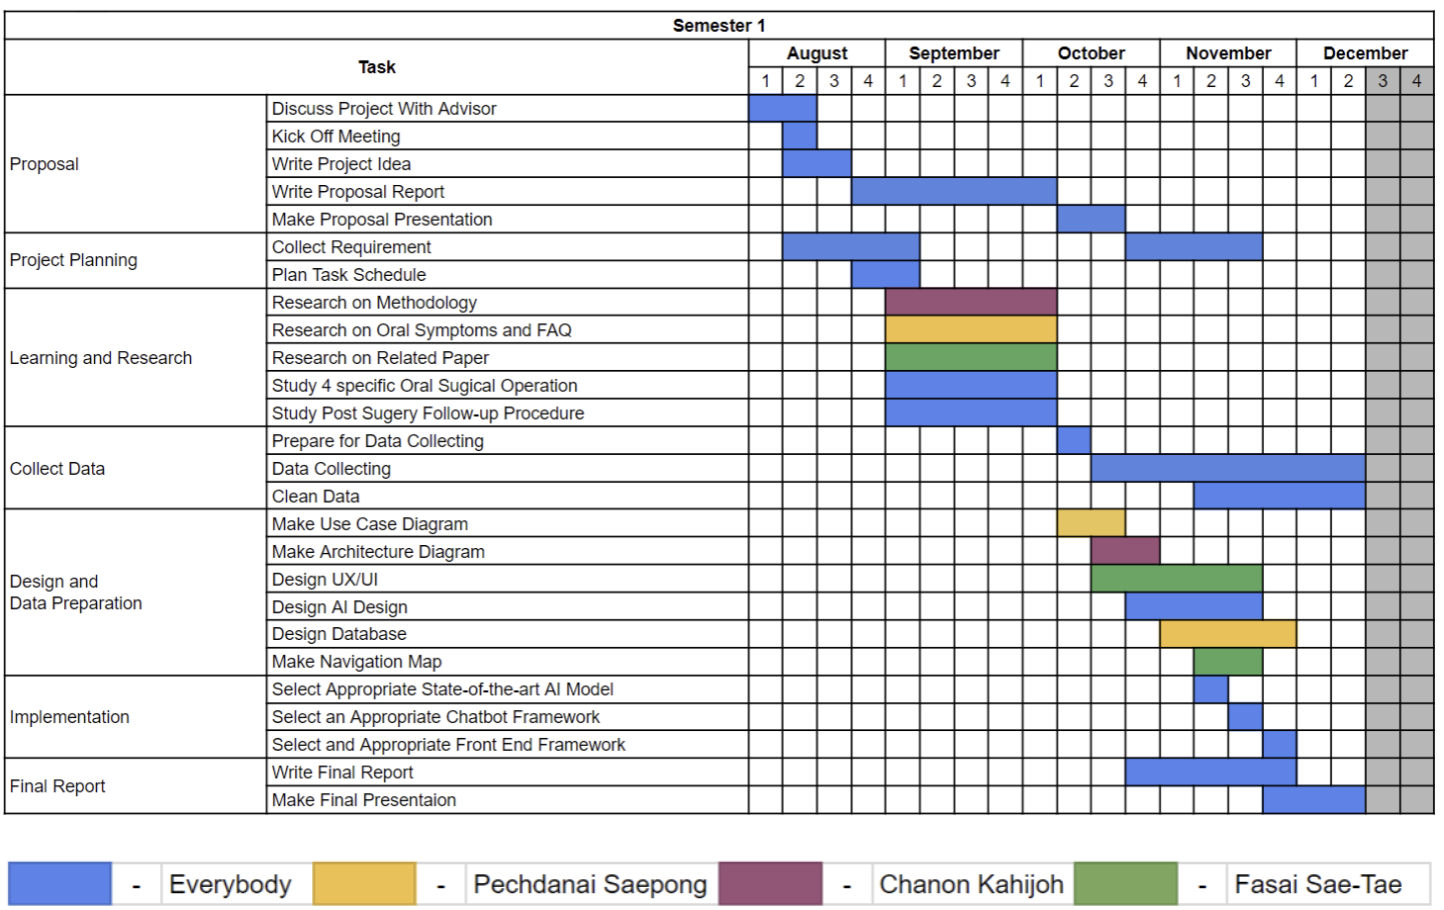
\includegraphics[width=.9\textwidth]{Image/Term1_Gantt.png}}
        \caption{Semester 1 plan schedule}\label{fig:Term1_Gantt}
      \end{figure}
      \begin{figure}[!h]
        \centering
        \fbox{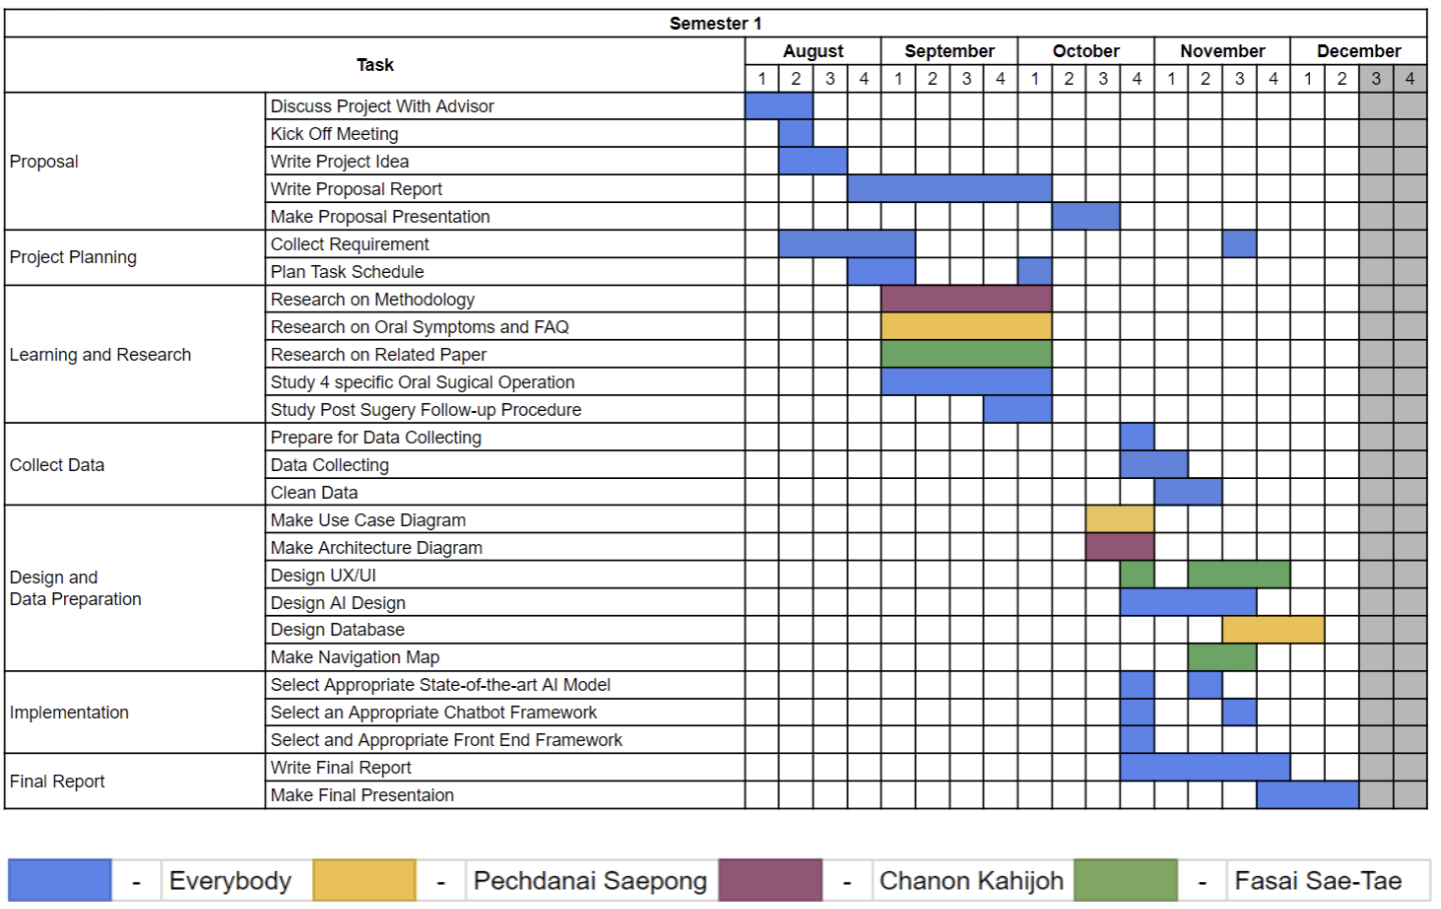
\includegraphics[width=.9\textwidth]{Image/Term1_Gantt_Actual.png}}
        \caption{Semester 1 actual schedule}\label{fig:Term1_Gantt_Actual}
      \end{figure}

    \subsection{Semester 2}
      \begin{enumerate}
        \item Deep Learning and Chatbot Implementation
          \begin{itemize}
            \item Model Implement
            \item Model Training
            \item Model Testing and Evaluation
          \end{itemize}
        \item Web Application Implementation
          \begin{itemize}
            \item Backend
            \item Frontend
            \item Test Case Design
            \item Unit Testing
            \item Usability Testing
          \end{itemize}
        \item Semester 2 Report
          \begin{itemize}
            \item Write Semester Report
            \item Semester Presentation
          \end{itemize}
      \end{enumerate}

    \subsection*{Deliverables for Term 2}
      \begin{itemize}
        \item Web application
        \item Line official Bot
        \item Testing result
        \item Feedback from users
        \item Senior Project Report
      \end{itemize}
      \begin{figure}[!h]
        \centering
        \fbox{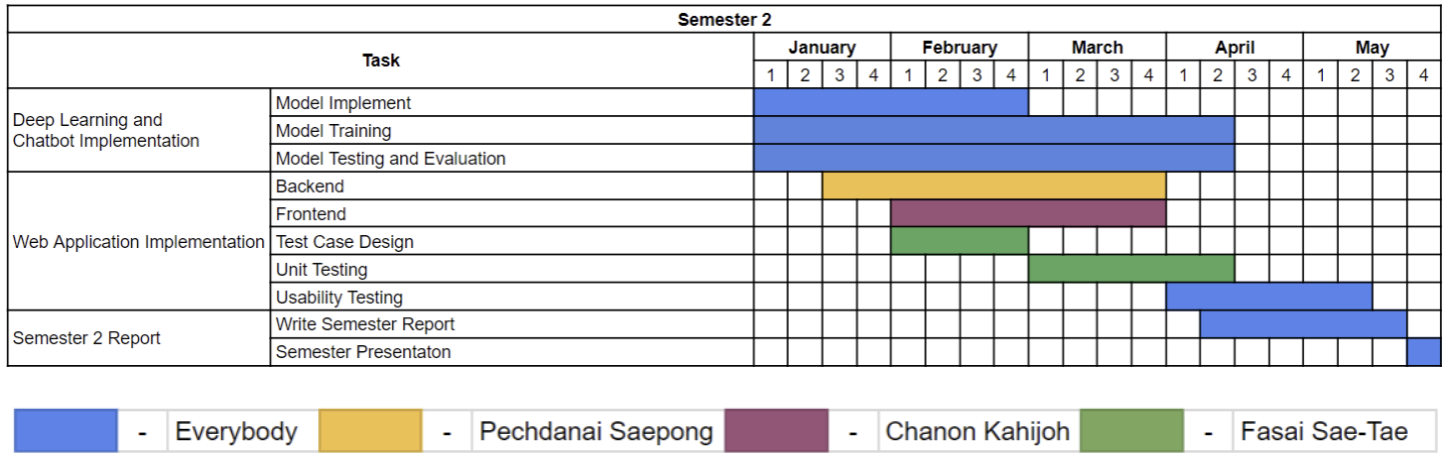
\includegraphics[width=.9\textwidth]{Image/Term2_Gantt.png}}
        \caption{Semester 2 plan schedule}\label{fig:Term2_Gantt}
      \end{figure}

\chapter{THEORY AND RELATED RESEARCH}
  \section{Introduction}
    \qquad This chapter will explain the details of the core concept and the solution planning. Theory and core concepts, languages and technologies, and related research will be discussed in this chapter. First, we will cover the theory and core concept of both dentistry and artificial intelligence. Second, programming languages and technologies that are intended to be used in this project will be described in the “Languages and Technologies” section. Lastly, related research and similar solution approaches to the objective will be discussed in the “Related Research and Competing Solutions” section.
    
  \section{Theory and Core Concepts}
    \qquad Common oral problems, including tooth decay, wisdom teeth complications, and gum disease, require consistent treatment for a considerable number of patients. Dentists, who routinely engage with patient inquiries and symptom tracking, have recommended that our focus be directed towards Tooth Extraction, Wisdom Tooth Removal, Periodontal Surgery, and Dental Implant Surgery. These specific procedures directly address the aforementioned common oral problems, aligning our work with the suggestions of dental professionals.\par
    \subsection{Tooth Extraction}
      \qquad Tooth extraction is a common dental procedure performed by a dentist or oral surgeon to remove a tooth from its socket in the jawbone. It is necessary for various reasons, including extensive tooth decay, crowding, tooth impaction, or as part of orthodontic treatment. Recovery typically takes a few days to a few weeks. The benefits of tooth extraction vary depending on the reason for the procedure. However, the disadvantages of tooth extraction often include challenges with chewing food and a potential loss of aesthetic appeal. Additionally, there may be complications that require careful monitoring, such as post-surgical swelling or infection.\par
    \subsection{Wisdom Tooth Removal}
      \qquad Wisdom tooth extraction, also known as third molar extraction, is a dental procedure performed to remove the third molars, commonly referred to as wisdom teeth. These teeth often become impacted or lead to various dental issues due to their slow growth and limited space in the jaw. Surgery becomes necessary for various reasons, including the prevention of pain arising from the inability of third molars to erupt properly or the prevention of issues related to crowded and misaligned teeth. However, the most common concerns associated with this procedure are the potential side effects after surgery, such as swelling, unusually significant or continuous discharge, or facial distortion lasting more than two weeks.\par
  
    \subsection{Periodontal Surgery}
      \qquad Periodontal surgery, also known as gum surgery, is a dental procedure aimed at treating various gum diseases and conditions. It involves the removal of infected gum tissue and, in some cases, the reshaping of the underlying bone to restore gum health and improve the stability of teeth. During this surgery, the dentist or periodontist carefully removes the diseased tissue and then shapes and contours the remaining gum and bone to promote optimal healing. In more advanced cases, bone grafts or tissue-stimulating proteins may be used to encourage tissue regeneration. Periodontal surgery is crucial in preventing the progression of gum diseases, reducing gum pockets, and ultimately preserving the natural teeth. Besides its significant impact on oral health, undergoing periodontal surgery can also enhance an individual's confidence and self-esteem by restoring a healthy, aesthetically pleasing smile.\par
  
    \subsection{Dental Implant Surgery}
      \qquad A dental implant is a technology used to replace missing teeth by employing sturdy materials as dental implants to serve as replacements for natural tooth roots. Presently, it is common to use dental implants that encompass both the root and the tooth, as they closely resemble natural teeth in appearance and function realistically. Additionally, they aid in preventing the deterioration of the jawbone where the implant is placed. To be a suitable candidate for dental implants, a patient must possess healthy gums and adequate bone support for the tooth roots. Following a root canal procedure, it is imperative for the patient to consistently maintain their oral health. Dental implants offer numerous advantages, including the prevention of teeth from shifting or becoming misaligned due to tooth loss, as well as contributing to the strengthening and preservation of oral hygiene.\par
  
  \section{Languages and Technologies}
    \subsection{Web Development Language}
      \subsubsection{JavaScript}
        \qquad JavaScript, abbreviated as JS and developed by Netscape in the mid-1990s, is one of the most used programming languages in web development. It enables the development of dynamic content within web pages, enhancing websites responsiveness to user interactions.\par
        \qquad Operating as a scripting language on the client side, JavaScript runs directly within web browsers, facilitating interaction with the Document Object Model (DOM), which represents a webpage's structure and content.\par
        \qquad JavaScript boasts a rich set of features and capabilities, including support for various data types, loops, functions, and more. Moreover, it offers many libraries and frameworks that simplify complex tasks.\par
        \qquad A key attribute of JavaScript is its capacity to handle asynchronous operations. Asynchronous operations enable data retrieval without disrupting the user’s experience, as these operations occur independently through mechanisms such as async/await and Promises.\par
      \subsubsection{TypeScript}
        \qquad Developed by Microsoft, TypeScript (or TS) is an enhanced version of JavaScript, adding strong typing and advanced features to the original language.\par
        \qquad One of the most noticeable changes from default JavaScript is the introduction of a strong tying system. TypeScript requires variables, function parameters, and function return types to be explicitly defined with data types. This enhances error detection during the development process, resulting in fewer bugs when the website is deployed. It also promotes easier cooperation between developers, as the code becomes more understandable.\par
        \qquad TypeScript offers additional features, such as interfaces and custom type definitions, which enable objects to have specific shapes. This feature enhances code comprehension and facilitates integration with third-party libraries.\par
      
      \subsubsection{Python}
        \qquad Python, famous for its ease of use and readability, has gained in popularity in web programming due to its flexibility and an extensive collection of frameworks designed for web application development. It is frequently employed in web backend development, offering developers a wide range of frameworks and libraries to choose from. This diversity makes it an attractive choice for creating robust and scalable websites.\par
  
      \subsubsection{Hypertext Markup Language}
        \qquad Hypertext Markup Language, abbreviated as HTML, serves as the standard language for creating the structural framework of websites. It uses a markup syntax consisting of tags to define various components, including headings, paragraphs, links, images, etc. HTML’s simplicity, adaptability, and compatibility with multimedia features have solidified its enduring importance in the realm of website development. It stands as an indispensable tool for developing everything from straightforward web pages to complex websites.\par
  
      \subsubsection{Cascading Style Sheet}
        \qquad Cascading Style Sheets, abbreviated as CSS, is commonly referred to as a "style sheet." It is a language used to format HTML documents, with CSS being responsible for defining rules that specify the presentation of content within a document. These rules encompass aspects such as text color, background color, font type, and text positioning. The fundamental concept behind CSS is the separation of HTML document content from the instruction used for formatting its display. By employing this separation, CSS achieves two primary objectives. Firstly, it ensures that the document's display format is independent of its content, facilitating the task of formatting HTML documents, especially when the content undergoes frequent changes. Secondly, CSS enables precise control over the presentation format of HTML documents, ensuring consistency across all pages within the same website. Styling rules for HTML documents were initially introduced in HTML 4.0 back in 1996, in the form of CSS Level 1 recommendations established by the World Wide Web Consortium (W3C).\par
    
    \subsection{Front-end Framework}
      \qquad Front-end frameworks play a crucial role in web development by simplifying the creation of user interfaces. They encompass design, layout, and interactive elements such as forms and buttons. These frameworks provide pre-written code that includes HTML, CSS, and JavaScript components, facilitating code reuse and maintaining consistency across web projects. By leveraging front-end frameworks, developers can efficiently generate HTML and CSS, design responsive layouts for various devices, ensure a consistent user experience, automate repetitive tasks, and manage their code efficiently. Ultimately, front-end frameworks streamline and structure the development process, enabling the creation of user-friendly and visually appealing web applications. Examples of front-end frameworks are as follows:\par
      \begin{itemize}
        \item React: A front-end framework, React stands apart because of its virtual Document Object Model (DOM), which enhances its functionality. It is a perfect framework for those who expect high traffic and require a steady platform to manage it. 
        \item Angular: Formally released in 2016, the Angular framework was established by Google to bridge the gap between the mounting demands of technology and conventional notions that displayed the results. In contrast to React, Angular is distinctive with its two-way data binding trait. It means that there is real-time synchronization between the view and model, where any alteration in the model replicates promptly on the view and vice versa.To reduce doctors and staff by minimizing repeated questions and explanations from patients.
        \item Vue.js: It has a small size and offers two main benefits – a visual DOM and a component-based structure. It also employs two-way data binding. This front-end framework is versatile and assists with various tasks when building web applications. The difference between Vue and React is that Vue is a JS framework while React is a JS library. So, Vue is more suitable for large projects.
        \item Semantic-UI: The objective of Semantic lies in empowering the designers and developers by creating a language for sharing UI. It uses natural language that makes the entire code self-explanatory. The framework is comparatively new to the ecosystem. Still, with its striking user interface, simple functionalities, and features, it has become one of the most popular front-end frameworks.
        \item Next.js: Used by some of the world's largest companies, Next.js enables you to create full-stack web applications by extending the latest React features and integrating powerful Rust-based JavaScript tooling for the fastest builds.
      \end{itemize}
  
    \subsection{Backend Framework}
      \qquad A backend framework serves as a foundational platform for developers to expedite the creation of web and mobile applications with standardization. In the context of backend frameworks, they simplify server-side development by offering tools, libraries, and components that streamline the construction of web applications. These frameworks automate various aspects of web development, enhancing efficiency and cleanliness in code design. Examples of backend frameworks are as follows:\par
      \begin{itemize}
        \item ExpressJS: It is a minimal Node.js framework used to develop highly flexible applications.
        \item Django: Django is the most popular Python framework used in web development. Based on the Don’t Repeat Yourself (DRY) principle, Django focuses on code reusing, thus enhancing the development speed. It is also a very secure framework.
        \item Node.js: JavaScript is the most popular programming language in the world. With the emergence of Node.js, JavaScript’s popularity in the backend development community increased rapidly, and in the last decade, Node.js has become one of the top names.
        \item Flask: It’s a simple, highly flexible, and performing web framework. Being a lightweight framework, or micro-framework, it is easy to learn and understand Flask. Moreover, being a Python framework, it is very user-friendly.
      \end{itemize}
    
    \subsection{Chatbot}
      \qquad A chatbot is a machine learning (ML) or artificial intelligence (AI) system designed to simulate and handle human conversations, whether written or spoken. These AIs enable users to interact with digital devices as if they were having a conversation with a human. Chatbots can vary widely in complexity, from basic systems that respond to user queries to advanced digital assistants that learn and adapt over time, providing personalized experiences as they collect and process data.\par
      \subsubsection{Chatbot Framework}
        \qquad A Bot Framework is a platform where developers create and define the behavior of chatbots. It simplifies the complex task of building chatbots that can operate on various messaging platforms and software development kits (SDKs). While some frameworks claim “write once, deploy anywhere" capabilities, in practice, developers often need to create separate chatbots for each messaging platform. The Bot Framework comprises components such as the Bot Builder SDK, Bot Connector, Developer Portal, Bot Directory, and an emulator for testing. However, it may not be the best choice for beginners looking to learn chatbot development due to its complexity.\par
        \qquad Examples of Bot frameworks include:\par
        \begin{itemize}
          \item DialogFlow
          \item Microsoft Bot Framework
          \item Rasa
          \item Amazon Lex
          \item IBM Watson Assistant
          \item Wit.ai
          \item Botpress
        \end{itemize}
      
      \subsubsection{Pretrained Chatbot Model}
        \qquad A pretrained chatbot model is a Natural Language Processing (NLP) model that has been trained on a wide range of text data from sources such as books, articles, social media, etc. These models are equipped with the capability to understand and generate text that closely resembles human language, making them valuable for chatbot development and other natural language tasks. These chatbots can also undergo fine-tuning or additional training for a specific task or domain to enhance their accuracy and performance.\par
        \paragraph{DeBERTa}\mbox{}\\
          \null\qquad DeBERTa (Decoding-enhanced BERT with disentangled attention) is a neural language model architecture designed to enhance the performance of pre-trained models like BERT (Bidirectional Encoder Representations from Transformers) and RoBERTa (Robustly optimized BERT approach) with two techniques, a disentangled attention mechanism and an enhanced mask decoder.\par
          \qquad The disentangled attention mechanism involves representing each word with two vectors—one for content and one for position. Attention weights among words are then calculated using disentangled matrices for content and relative positions, allowing the model to independently consider semantic content and positional relationships during computations.\par
          \qquad The enhanced mask decoder replaces the output softmax layer to predict masked tokens during model pre-training. Additionally, a new virtual adversarial training method is applied during fine-tuning to enhance the model's generalization for downstream tasks.\par
          \qquad The DeBERTa V2 model is a variant of the transformer architecture designed for question-answering tasks. Its structure consists of an embedding layer for word representations, employing layer normalization and dropout for regularization. The core encoder is composed of multiple DeBERTa V2 layers, each featuring a disentangled self-attention mechanism, an intermediate layer with GELU activation, and output layers for attention and transformation. The model incorporates relative positional embeddings to efficiently capture token dependencies. The final layer includes a linear output module specialized for predicting start and end positions in the input sequence, crucial for question answering. Overall, DeBERTa V2 integrates advanced attention mechanisms and positional embeddings to enhance its ability to capture complex relationships within the input data for improved performance in question-answering tasks.\cite{deberta1,deberta2}\par
  
        \paragraph{mDeBERTa}\mbox{}\\
          \null\qquad mDeBERTa\cite{huggingface1} is the multilingual version of DeBERTa. Both models have the same architecture but mDeBERTa supports multiple languages while DeBERTa supports only English.\par
      
    \subsection{Machine Learning}
      \qquad Machine Learning (ML) is a branch of Artificial Intelligence that tries to replicate how humans work. It uses the accumulated data in order to let machines learn step by step in order to improve its accuracy in the task they are trained to do.\par
        
        \subsubsection{Decision Tree}
          \qquad A decision tree is a supervised machine learning algorithm used for categorizing and regression tasks. A decision tree consists of root node, decision nodes, leaf nodes, splitting, pruning, and branches.\par
          \qquad The decision tree operates by employing various algorithms to decide to split a node into two or more sub-nodes. Decision trees work by iteratively partitioning nodes based on all available features and subsequently selecting the split that leads to the most uniform or homogeneous sub-nodes in terms of the target variable. This aims to create clear and distinct decision boundaries within the dataset, facilitating more accurate predictions or classifications by the decision tree model.\cite{decisiontree1}\par
          \begin{figure}[!h]
            \centering
            \fbox{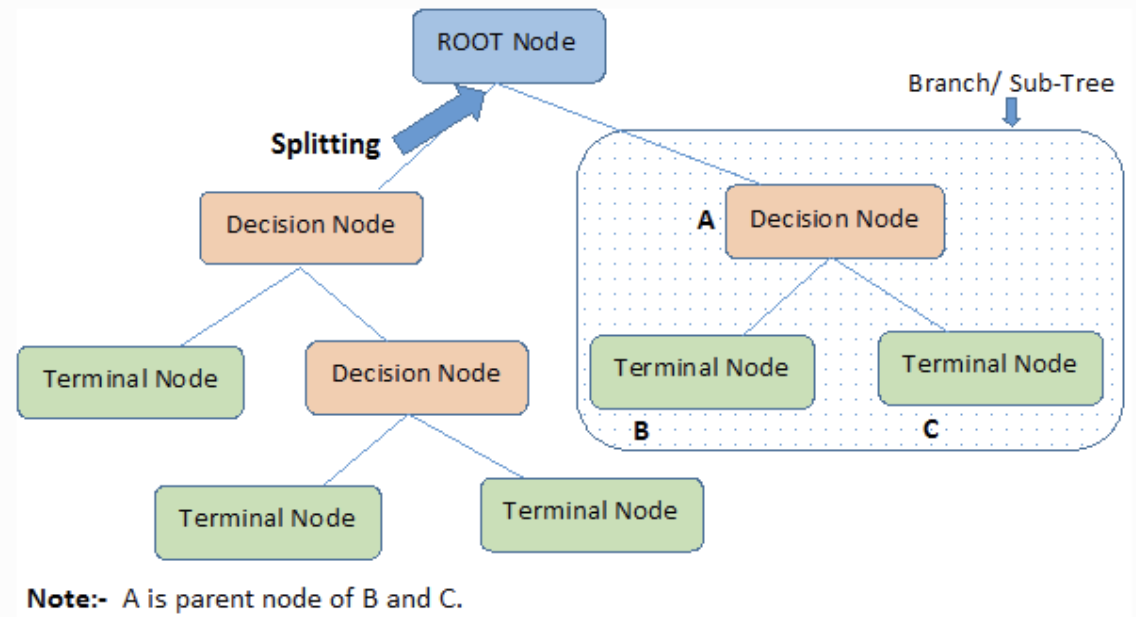
\includegraphics[width=.6\textwidth]{Image/Decision_Tree.png}}
            \caption{Diagram explaining Decision Tree\cite{decisiontree2}}\label{fig:Decision_Tree}
          \end{figure}
        
        \subsubsection{Random Forest}
          \qquad Random Forest is the combination of many decision trees and using results from all decision trees by either averaging or majority voting making it less biased which helps in overfitting problems. As you can see from Figure 1.2, the final results are obtained after getting results from many decision trees.\par
          \begin{figure}[!h]
            \centering
            \fbox{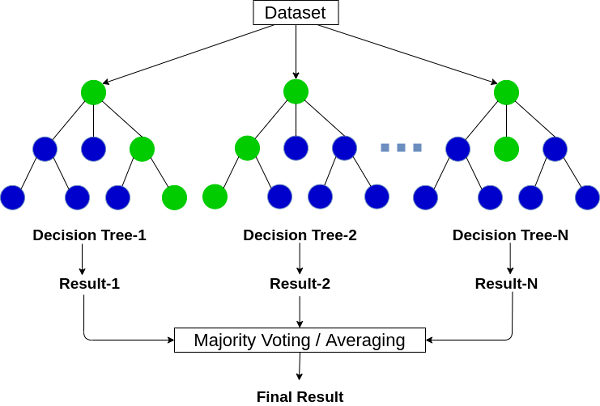
\includegraphics[width=.6\textwidth]{Image/Random_Forest.png}}
            \caption{Diagram explaining Random Forest}\label{fig:Random_Forest}
          \end{figure}
        \subsubsection{Naive Bayes}
          \qquad Naive Bayes uses the Bayes theorem where it calculates the probability of event A based on the past data given. In Naive Bayes it applies this theorem with the ‘Naive’ assumption that the features are independent of each other.\cite{NaïveBayes1, NaïveBayes2}\par 
          \begin{equation}
            P(y|X) = \frac{P(X|y) * P(y)}{P(X)}
          \end{equation}
          \qquad This Bayes theorem formula shows X is a feature vector  X=(x1,x2,…,xn) and y is class. And due to the naive assumption, which can be dictate with \par
          \begin{equation}
            P(X|y) = P(x_1|y) * P(x_2|y) \ldots P(x_n|y) * P(y)
          \end{equation}
          \qquad Thus naives bayes formula can be shown as: \par
          \begin{equation}
            P(y|X) = \frac{P(x_1|y) * P(x_2|y) \ldots P(x_n|y) * P(y)}{P(x_1) * P(x_2) \ldots P(x_n)}
          \end{equation}
          \qquad Which can then be simplified as: \par
          \begin{equation}
            P(y|x_1,x_2,\ldots,x_3) \propto P(y) \prod\limits_{i=1}^{n} P(x_i|y)
          \end{equation}
    \subsection{Keyword Search}
      \qquad For keyword search we have 2 types. One of them uses normal search word search in a sentence while another uses Regular Expression, or Regex for short, in order to find a word in a sentence. Using Regex will allow the word to be searched even if there are typing mistakes in the word such as typing \textthai{ถอมฟัน} instead of \textthai{ถอนฟัน}. The cases that we included for this regular expression is having a letter swapped, added or removed. \par

    \subsection{Augmenting Data}
      \qquad We augmented text data to expand data while trying to simulate human error such as misspelling a word or typing a key by mistake. We can achieve this by inserting random characters into the questions, deleting random characters in the questions, and swapping random characters in the questions. We are also able to expand by paraphrasing the sentence. In order to have the best performance for paraphrasing we need to first translate it to English then let the AI model\cite{huggingface2} paraphrase as it is an English paraphrasing model then translate the results back to Thai.\par
    \subsection{Proposed Framework}
      \qquad The proposed framework has 3 components that are to be used together:\par
      \begin{itemize}
        \item Keyword Search: classify the input question into each operation        
        \item Random Forest: classify the input question into class
        \item BERT: answer the user's question based on the identified class
      \end{itemize}
      \qquad We first input a question into a keyword search algorithm and random forest model in order to classify which classes, operation and question type respectively, it belongs to. We then input that class in order to use the correct context in order to get the correct answer. With this method we can reduce time taken while trying to increase qa model accuracy. \par
  \section{Related research / Competing solutions}
    \subsection{Related Research}
      \qquad \textbf{Designing a Competent Chatbot to Counter the COVID-19 Pandemic and Empower Risk Communication in an Emergency Response System}\par
      \begin{figure}[!h]
        \centering
        \fbox{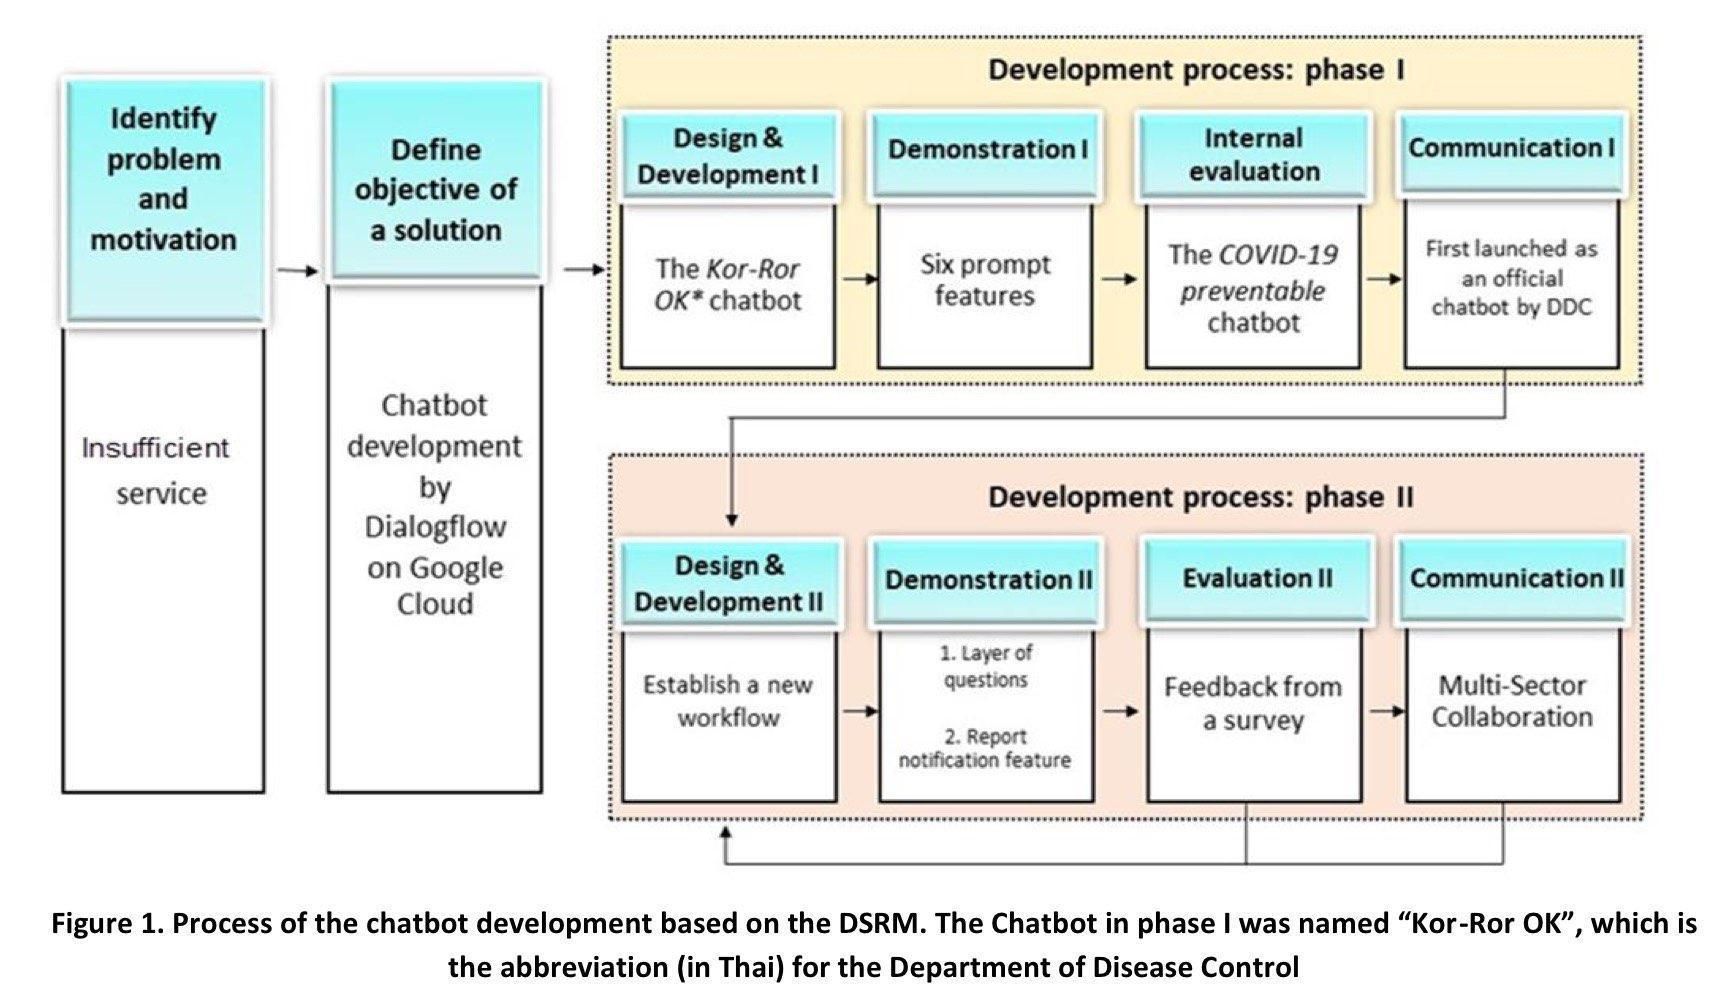
\includegraphics[width=.6\textwidth]{Image/Research_1.jpg}}
        \caption{Overview of DSRM development process\cite{relatedwork1}}\label{fig:Research_1}
      \end{figure}
      \qquad This paper presented the development process and the characteristics of a competent chatbot, with an emphasis on COVID-19. The paper used Design Science Research Methodology (DSRM) as the development process to implement the chatbot, which consisted of 6 steps. Line Application was chosen as the main channel for the development and was deployed using Dialog Flow. In phase one, the development focused on implementing a chatbot capable of answering various frequently asked questions and providing knowledge about COVID-19. The emphasis shifted to more complex questions and chatbot efficiency in phase 2 of the development.\par
      \qquad The knowledge in this paper regarding the development process can be used and applied to our development process since the output products are similar in terms of use. However, the step of product evaluation will be different since we do not have a large number of users, and some key features, such as follow-up, are different.\par
    \subsection{Competing Solution}
      \subsubsection{DentalChat}
        \begin{figure}[!h]
          \centering
          \fbox{
\includegraphics[width=.2\textwidth]{Image/DentalChat_Logo.png}}
          \caption{DentalChat Logo\cite{dentalchat}}\label{fig:DentalChat_Logo}
        \end{figure}
        \qquad DentalChat is an AI dental care application that connects and allows users to ask dental questions and is assisted by a dentist in real-time. DentalChat features consist of finding a local dentist, asking dental questions, post consult requests, and chatting with the dentist.\par
      \subsubsection{PsyJai}
        \begin{figure}[!h]
          \centering
          \fbox{
\includegraphics[width=.2\textwidth]{Image/PsyJai_Logo.png}}
          \caption{PsyJai Logo\cite{psyjai}}\label{fig:PsyJai_Logo}
        \end{figure}
        \qquad PsyJai is a comprehensive automated AI mental health assistance system collaboration that can perform mental health assessments and provide psychological care based on the principles of psychology. PsyJai provides services through Facebook and Line. PsyJai has 4 main features: 1. Emotional Status Screening 2. Basic Care with Psychological Principles 3. General Conversations 4. Mood Dashboard.\par
      \subsection{Comparison Table}
        \begin{table}[h]
          \centering
          \caption{\centering Comparison table between our proposed solution, DentalChat and PsyJai}\label{tab:Comparison_Table}
          \begin{tabular}{|c|c|c|c|} \hline
            & Our proposed Solution & DentalChat & PsyJai \\\hline
            Symptom Diagnosis & AI System & Manual & AI System \\\hline
            Post-Surgery Follow-Up & AI System & - & - \\\hline
          \end{tabular}
        \end{table}
        \qquad According to Table 1, our proposed solution has 2 main features: symptom diagnosis and post-surgery follow-up, both of which are AI-based systems. In contrast, DentalChat only has a symptom diagnosis feature, which is manually answered by the doctors. Psyjai also has an AI-based system for symptom diagnosis but does not have the post-surgery follow-up feature.\par

\chapter{DESIGN AND METHODOLOGY}
  \section{Introduction}
  \qquad This chapter will cover the features, architecture, functionalities, design methods, and diagrams of our web application. We will delve into the details of the application’s functionality and architecture. \par
  \section{Project Functionality}
    \subsection{System Requirements}
    \begin{itemize}
      \item The web application must allow users to log in via Line Account.
      \item The web application must automatically log in users accessing via Line.
      \item The web application must facilitate all users in asking frequently asked questions through a chatbot.
      \item The web application must enable logged-in users to scan a QR code to create a new follow-up case.
      \item The web application must allow logged-in users to respond to follow-up chatbot queries.
      \item The web application must permit logged-in users to view their individual profiles.
      \item The web applications must provide the option for all logged-in users to log out.
      \item The line chat should be able to do both Follow-Up and FAQ Chatbot
    \end{itemize}

    \subsection{Feature List}
      \subsubsection{Patient Registration}
      \qquad This feature entails user registration for the web application, accessible through Line Official. Upon the user’s initial accesses to the web application via Line Official, they are required to authorize the linking of their Line account. Once authorized, subsequent accesses to the web application through Line Official menu will result in automatic user login. \par
      \subsubsection{Frequently Asked Questions Answering Chatbot}
      \qquad This feature is designed to provide information and address common inquiries concerning distinct surgical procedures, including Tooth Extraction, Wisdom Tooth Removal, Periodontal Surgery, and Dental Implant Surgery. Users can input questions related to these surgeries, and the chatbot will provide pertinent information. In instances where the chatbot encounters unfamiliar questions that it cannot answer, it will return an error message and retain the question for future training purposes. \par
      \subsubsection{Follow-Up Chatbot}
      \qquad This feature aims to streamline the post-surgery monitoring process by replacing traditional methods where medical staff make follow-up calls to assess patients' conditions. The proactive chatbot targets follow-up questions based on the patient’s surgery, gathering insights into their current state for condition assessment and providing relevant advice. \par
      \subsubsection{Add New Follow-Up Case}
      \qquad This feature enables users to initiate a new follow-up case by scanning a provided QR code at the healthcare unit and selecting the undergone operation. \par
      \subsubsection{View Past Follow-Up Case}
      \qquad This feature allows users to review their history of past follow-up cases. 

  \section{Overall System Flow}
    \qquad The user will interact with only the client side of the web application and the Line Official Bot. The user will login to the web application using line and will receive notification about follow-up via line application as well. The chatbot model will be hosted by dialogflow and hugging face and the server will be able to use those using API requests while also querying from the database. \par
    \begin{figure}[!h]
      \centering
      \fbox{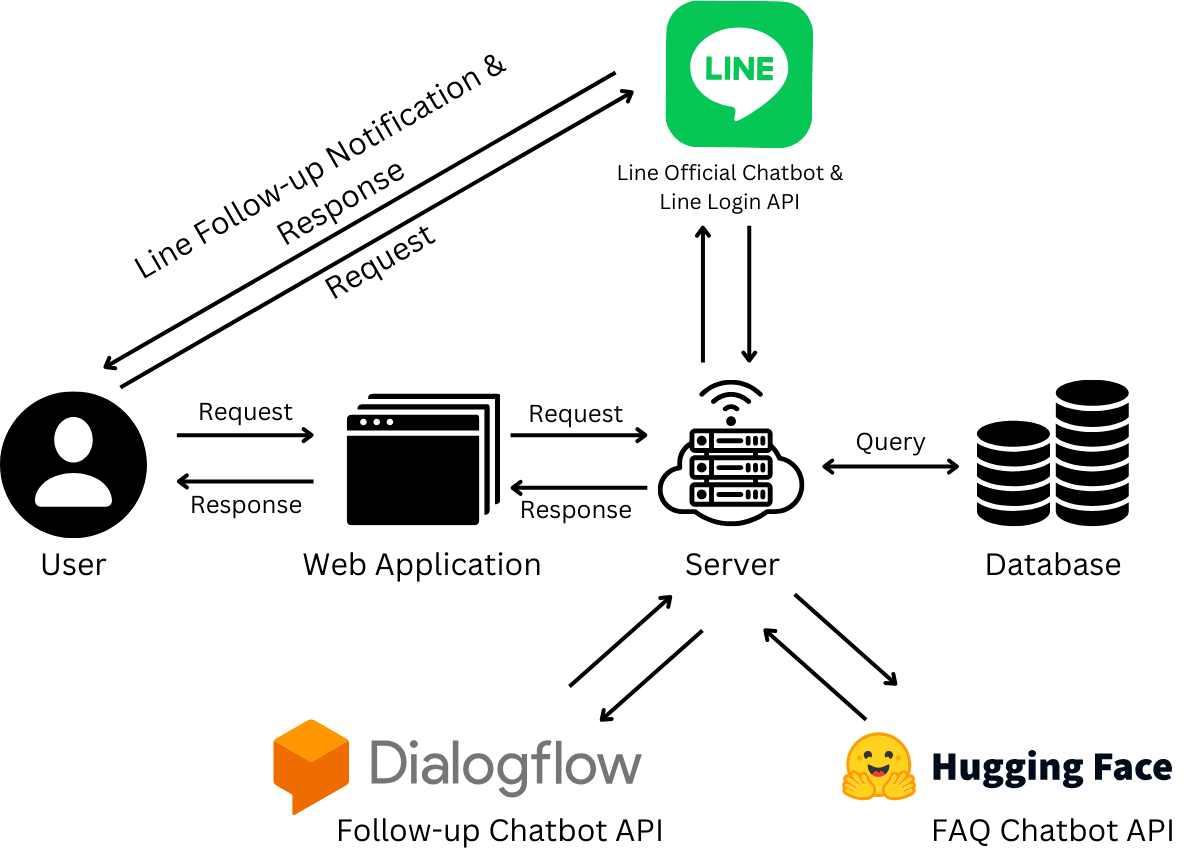
\includegraphics[width=.5\textwidth]{Image/Overall_System_Flow.png}}
      \caption{Overall System Flow}\label{fig:Overall_System_Flow}
    \end{figure}
  \section{System Architecture}
  \begin{figure}[!h]
    \centering
    \fbox{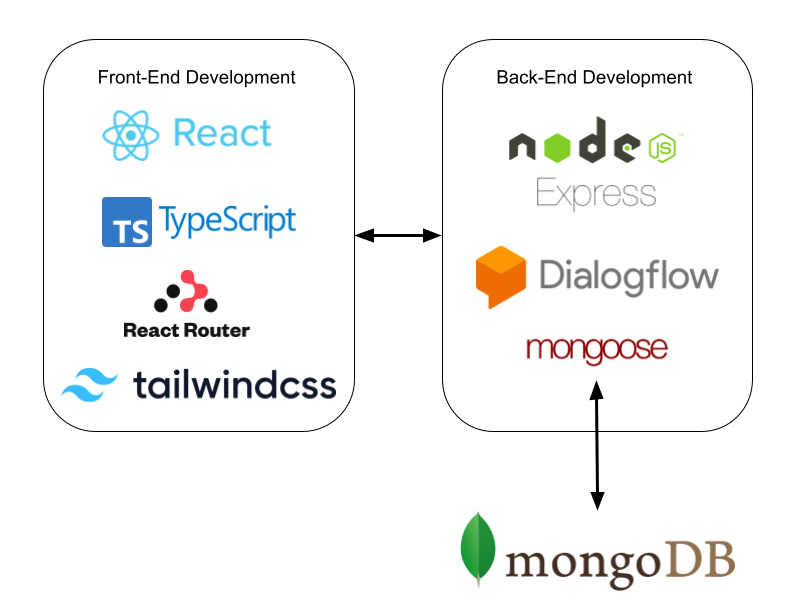
\includegraphics[width=.45\textwidth]{Image/System_Architecture.png}}
    \caption{Architecture Diagram}\label{fig:System_Architecture}
    \begin{flushleft}
      \qquad In the Figure 3.1 above, show the architecture design of our project. The Technology that we use in this project include. \par
      \begin{itemize}
        \item[] 1. React (Front-end JavaScript library for building UI)
        \item[] 2. React Router (React Router enables "client side routing")
        \item[] 3. TailwindCSS (CSS framework for styling the UI and used with React)
        \item[] 4. Node.js (Back-end JavaScript runtime environment)
        \item[] 5. Express (Back-end framework for Node.js for building REST API)
        \item[] 6. MongoDB (NoSQL Database)
        \item[] 7. Mongoose (Node.js based Object Data Modelling (ODM) library for MongoDB)
        \item[] 8. Flask (Python web framework for develop both front-end and back-end)
        \item[] 9. Dialogflow (employed for Follow-Up using its API to reduce resource usage in the client’s browser.)
      \end{itemize}
    \end{flushleft}        
  \end{figure}

  \newpage
  \section{Use Case Diagram}
  \begin{figure}[!h]
    \centering
    \fbox{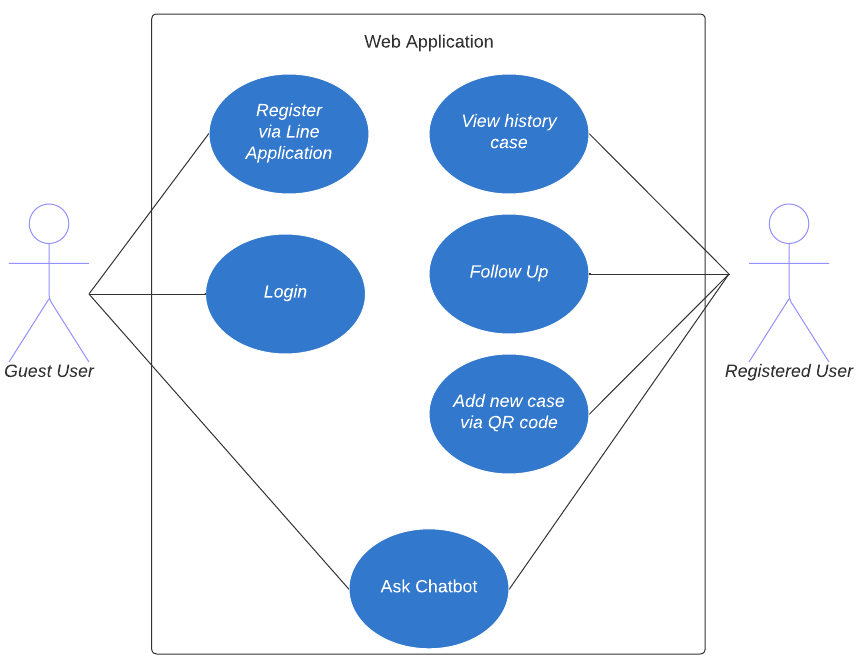
\includegraphics[width=.45\textwidth]{Image/Use Case Diagram - web.png}}
    \fbox{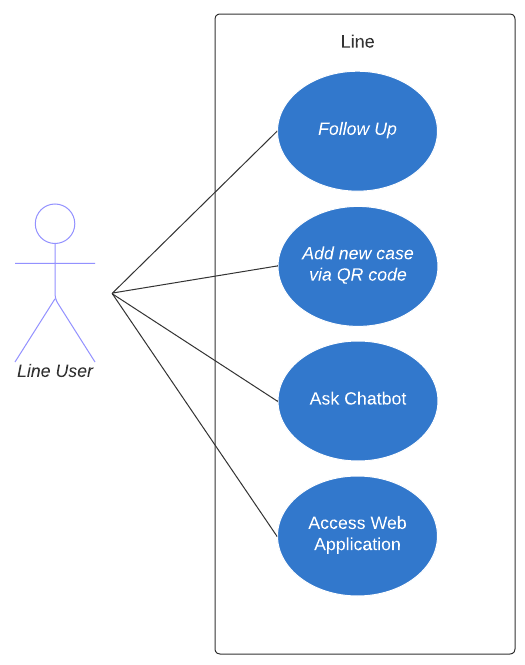
\includegraphics[width=.3\textwidth]{Image/Use Case Diagram - line.png}}
    \caption{Use Case Diagram of Web (Left) and Line (Right)}\label{fig:Use_Case}
  \end{figure}

  \section{Use Case Narrative}
    \subsection{Question Answer}
      \qquad Use case name: Question Answer \par
      \qquad Actors: All Uses \par
      \qquad Goal: Users ask questions and receive answers \par
      \qquad Preconditions: - \par
      \qquad Main success scenario:
      \begin{itemize}
        \item[] 1. Users go to the home page.
        \item[] 2. User selects the chatbot button.
        \item[] 3. User inputs a question.
        \item[] 4. System provides an answer to the question.
      \end{itemize}
      \qquad Extension (a)
      \begin{itemize}
        \item[] 1a. User goes to the Line Official Bot.
        \item[] 2a. User inputs a question.
        \item[] 3a. System provides an answer to the question.
      \end{itemize}

    \subsection{Login}
      \qquad Use case name: Login \par
      \qquad Actors: General Users \par
      \qquad Goal: Users log in to the system \par
      \qquad Preconditions: User is already registered (connected to Line account) \par
      \qquad Main success scenario:
      \begin{itemize}
        \item[] 1. User go to website homepage
        \item[] 2. User selects the “Login with Line Application” button
        \item[] 3. System navigates to the Line page and sets the token to this account.
        \item[] 4. System navigates the user to the FAQ page.
      \end{itemize}

      \subsection{Register (connected to Line account)}
        \qquad Use case name: Register \par
        \qquad Actors: General Users \par
        \qquad Goal: Add a new user to the system \par
        \qquad Preconditions: User has never connected to Line account \par
        \qquad Main success scenario:
        \begin{itemize}
          \item[] 1. User goes to the website homepage.
          \item[] 2. User selects the “Login with Line” button.
          \item[] 3. System navigates to the Line official login page.
          \item[] 4. User selects the “Allow” button.
          \item[] 5. System adds the new user.
        \end{itemize}
        \qquad Extension (a)
        \begin{itemize}
          \item[] 1a. System adds the new user.
          \item[] 2a. User searches for Line Official Bot.
          \item[] 3a. User adds Line Official.
          \item[] 4a. User selects the “Allow” button. 
          \item[] 5a. System adds the new user.
        \end{itemize}
      
      \subsection{Follow-Up}
        \qquad Use case name: Follow-Up \par
        \qquad Actors: Registered User (Patient) \par
        \qquad Goal: Registered User answers follow-up questions, and the system provides suggestions \par
        \qquad Preconditions: User has undergone surgery and scanned the QR code \par
        \qquad Main success scenario:
        \begin{itemize}
          \item[] 1. User logs into the system.
          \item[] 2. System presents follow-up questions.
          \item[] 3. Logged-in user answers the questions.
          \item[] 4. The answer pertains to the question.
          \item[] 5. System analyzes and offers suggestions to the patient.
        \end{itemize}
        \qquad Extension (a)
        \begin{itemize}
          \item[] 4a. The answer does not correspond to the question.
          \item[] 5a. System sends an error message and returns to step 2.
        \end{itemize}

      \subsection{View Case History}
        \qquad Use case name: View Case History \par
        \qquad Actors: Registered User (Patient) \par
        \qquad Goal: Registered User (Patient) accesses the user case page \par
        \qquad Preconditions: User has undergone surgery \par
        \qquad Main success scenario:
        \begin{itemize}
          \item[] 1. User logs into to the system.
          \item[] 2. System navigates to the FAQ page.
          \item[] 3. User selects the “Profile” button.
          \item[] 4. User accesses the Profile page displaying case history.
        \end{itemize}
        \qquad Extension (a)
        \begin{itemize}
          \item[] 1a. User logs into the Line Official Bot
          \item[] 2a. User selects the “View Case” button.
        \end{itemize}

      \subsection{Add New Case via QR Code}
        \qquad Use case name: Add New Case via QR Code \par
        \qquad Actors: Registered User (Patient) \par
        \qquad Goal: Registered User (Patient) adds a new case to the system\par
        \qquad Preconditions: User has undergone surgery. \par
        \qquad Main success scenario:
        \begin{itemize}
          \item[] 1. User logs into the system.
          \item[] 2. User selects “Scan QR Code” in the Line Official Bot or Web application..
          \item[] 3. User scans the QR code.
          \item[] 4. User gains access to the form.
          \item[] 5. User selects a treatment operation.
          \item[] 6. User submits the form to the system.
        \end{itemize}

\newpage
    \section{Activity Diagram}
      \subsection{Question Answering}
      \begin{figure}[!h]
        \centering
        \fbox{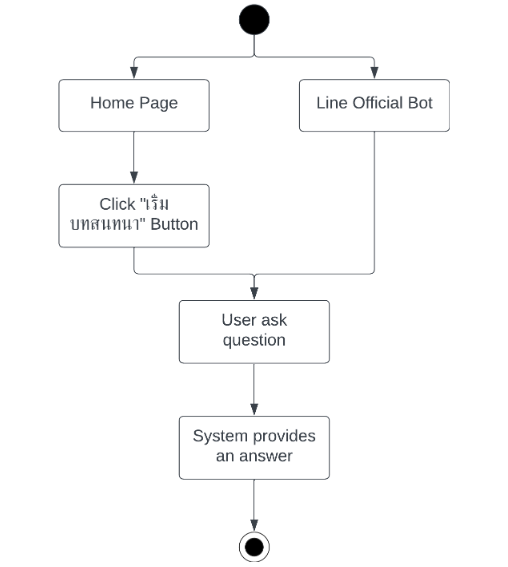
\includegraphics[width=.15\textwidth]{Image/AD_FAQ.png}}
        \caption{Question Answering Activity Diagram}\label{fig:AD_FAQ}
        \begin{flushleft}
          \qquad When users access the homepage and click the “\textthai{เริ่มบทสนทนา}” button, the system will display the chatbot interface. Users can then input their questions into the provided text box, and the system will respond with the appropriate answer to the question. \par
          \qquad Alternatively, if users access via Line Official Bot, users can then input their question to Line Official Bot and can receive the appropriate answer to the question from the system. \par
        \end{flushleft}
      \end{figure}

      \subsection{Login}
      \begin{figure}[!h]
        \centering
        \fbox{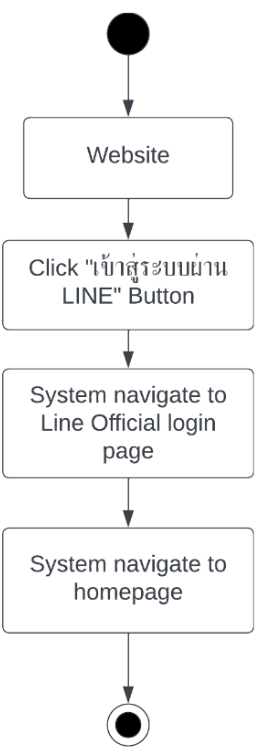
\includegraphics[width=.15\textwidth]{Image/AD_Login.png}}
        \caption{Login Activity Diagram}\label{fig:AD_Login}
        \begin{flushleft}
          \qquad When users access the homepage and click the “\textthai{เข้าสู่ระบบผ่าน} LINE”, the system will redirect the user to the Line page and subsequently navigate them to the FAQ page. \par
        \end{flushleft}
      \end{figure}
\newpage
      \subsection{Register}
      \begin{figure}[!h]
        \centering
        \fbox{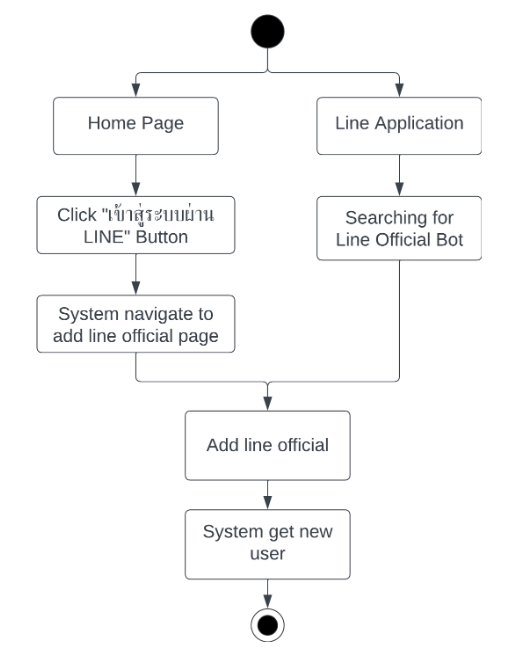
\includegraphics[width=.4\textwidth]{Image/AD_Regis.png}}
        \caption{Register Activity Diagram}\label{fig:AD_Register}
        \begin{flushleft}
          \qquad When users access the homepage and click the “\textthai{เข้าสู่ระบบผ่าน} LINE” button, the system will direct the user to the “Add Line Official” page. If the user clicks “Add Line Official” there, the system will automatically register this user.  \par
          \qquad Alternatively, if a user accesses via the Line application, search our Line Official Bot and then add our Line Official Bot, the system will also automatically register this user.  \par
        \end{flushleft}
      \end{figure}

      \subsection{Follow-Up}
      \begin{figure}[!h]
        \centering
        \fbox{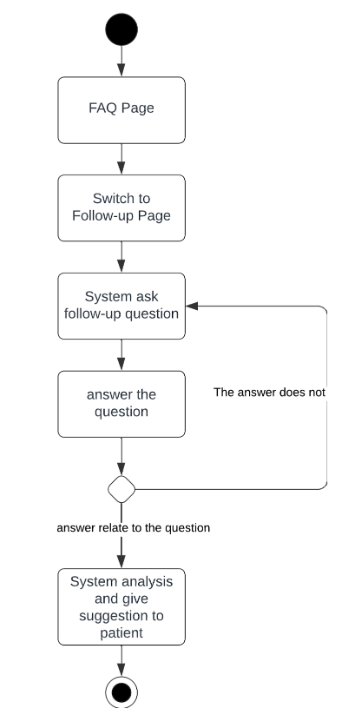
\includegraphics[width=.12\textwidth]{Image/AD_Follow.png}}
        \caption{Follow-Up Activity Diagram}\label{fig:AD_Follow}
        \begin{flushleft}
          \qquad When users access the FAQ page after completing the login process and subsequently switch to the Follow-up page, the system will present the follow-up chatbot interface. The system will then initiate by asking a follow-up question. Upon receiving the user’s answer, the system will analyze it and provide a suggestion to the user. However, if the answer does not pertain to the question asked, the system will attempt to reask the question to obtain a related answer from the user.   \par
        \end{flushleft}
      \end{figure}
\newpage
      \subsection{View Case History}
      \begin{figure}[!h]
        \centering
        \fbox{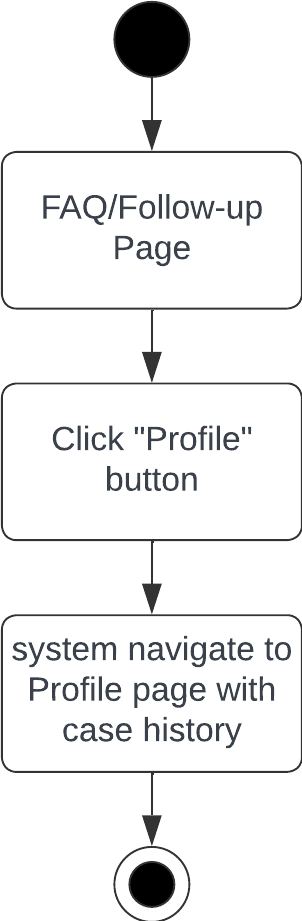
\includegraphics[width=.15\textwidth]{Image/AD_ViewCase.png}}
        \caption{View case history Activity Diagram}\label{fig:AD_ViewCase}
        \begin{flushleft}
          \qquad When users access the FAQ or Follow-up page and click on the “Profile” button, the system will direct them to the profile page, displaying their case history.  \par
          \qquad Alternatively, if users access via our Line Official Bot and click on the “View Case” button, the system will display all users' cases. \par
        \end{flushleft}
      \end{figure}
\newpage
      \subsection{Add New Case via QR Code}
      \begin{figure}[!h]
        \centering
        \fbox{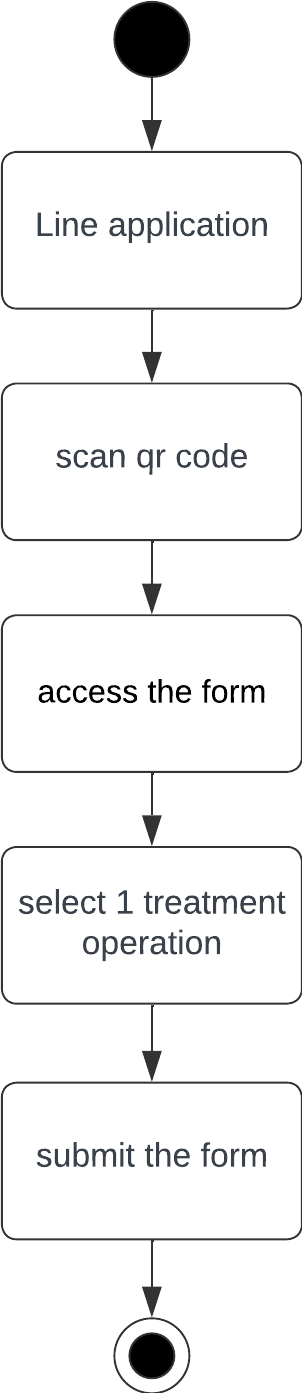
\includegraphics[width=.12\textwidth]{Image/AD_AddCase.png}}
        \caption{Add new case via QR code Activity Diagram}\label{fig:AD_AddCase}
        \begin{flushleft}
          \qquad When users open the Line application and scan our QR code, they will access a form where they need to select one of the treatment operations and submit the form.  \par
          \qquad Alternatively, if users access via profile or follow-up page in web application and click “+” button and scan our qr code they will also access a form where they need to select one of the treatment operations and submit the form. \par
        \end{flushleft}
      \end{figure}

  \section{Navigation Map}
    \begin{figure}[!h]
      \centering
      \fbox{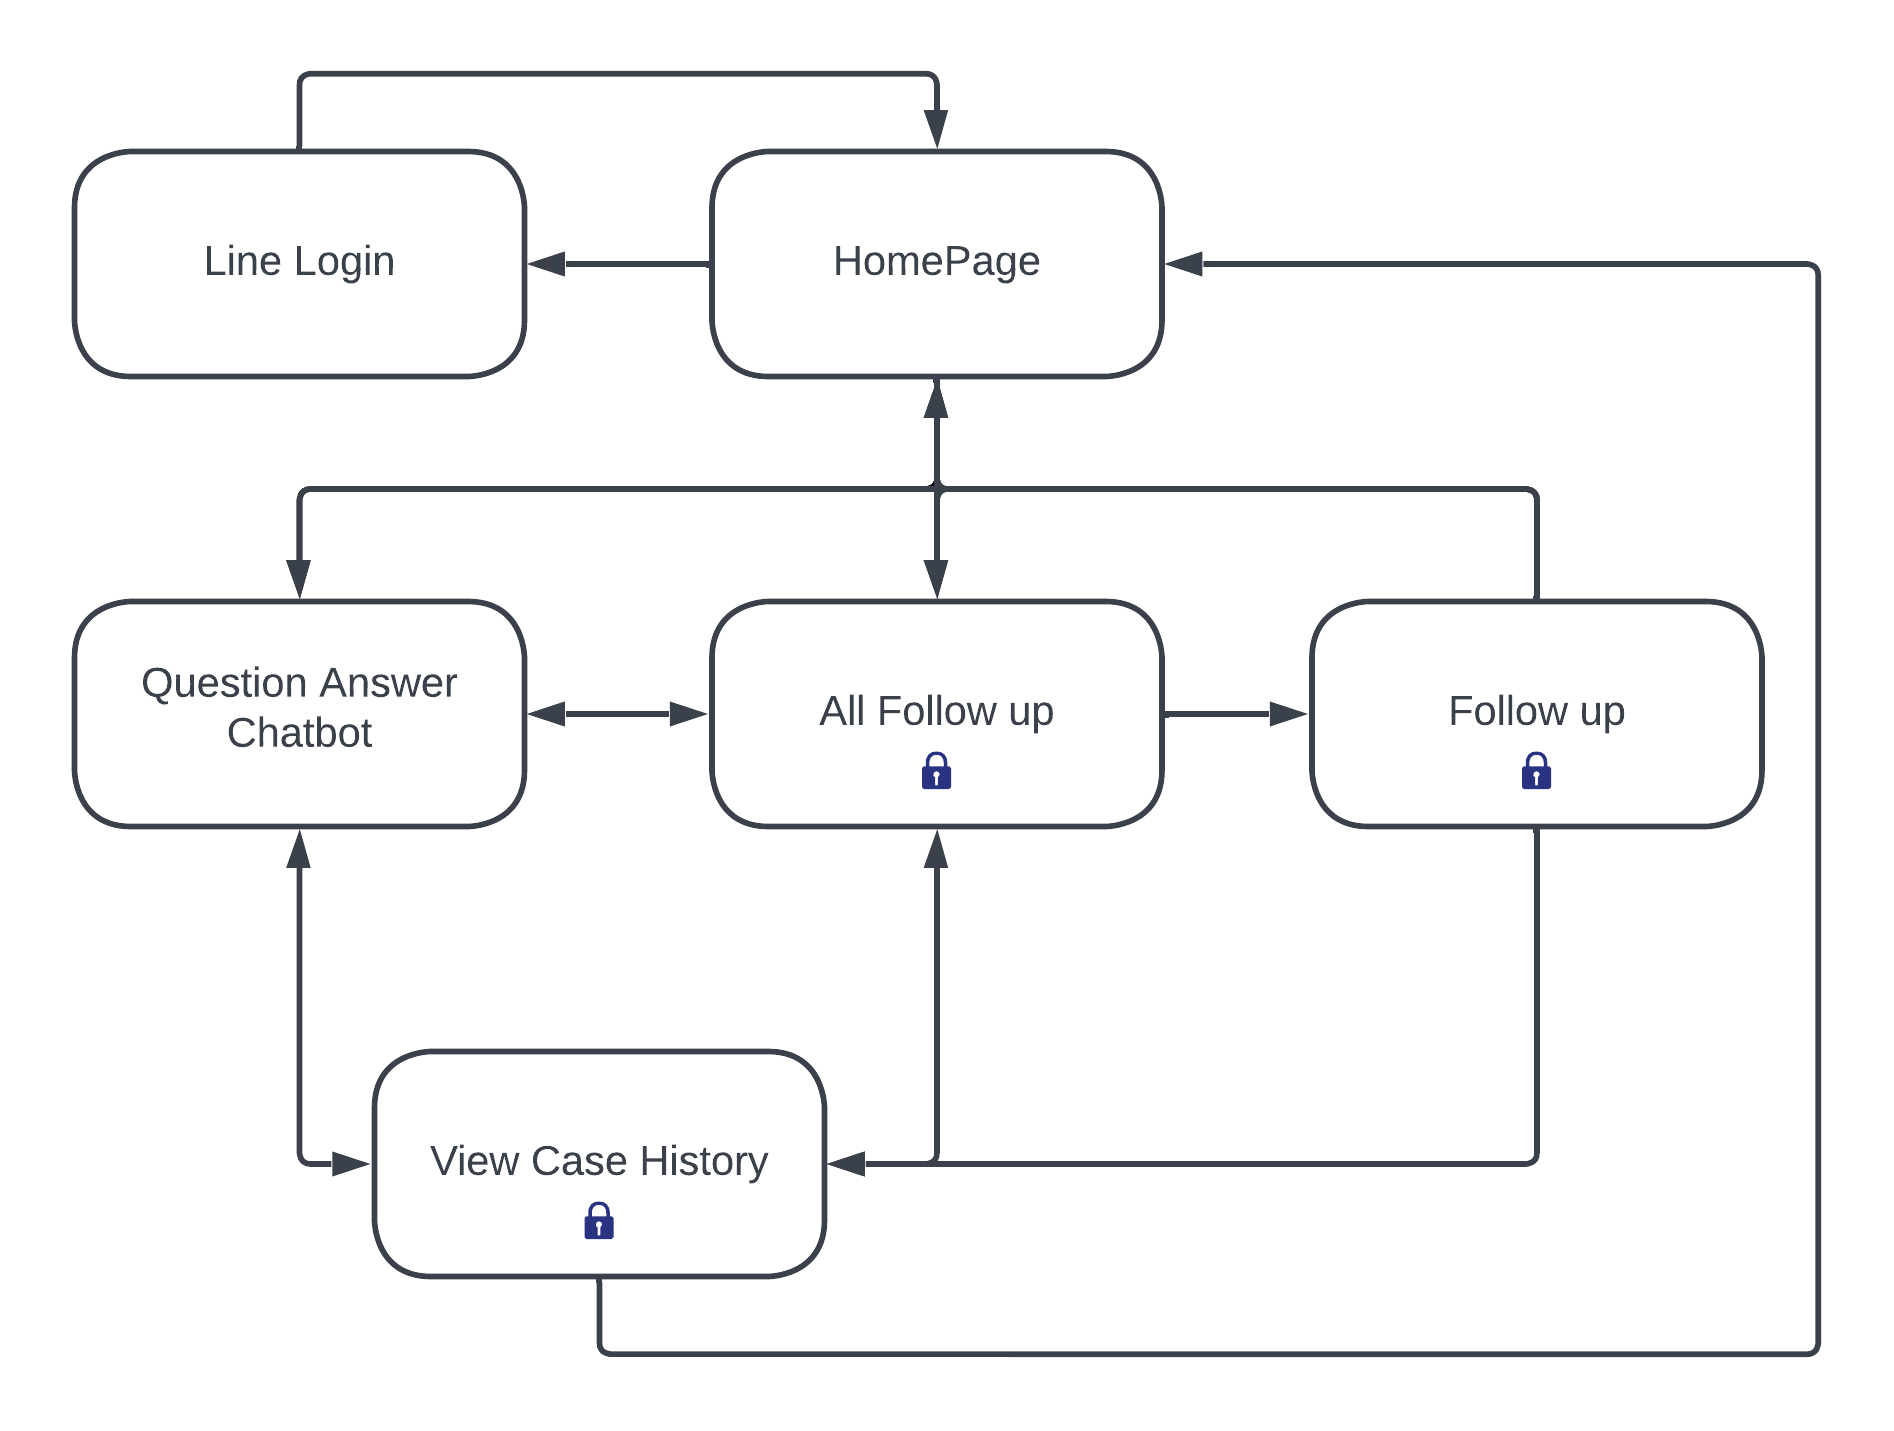
\includegraphics[width=.4\textwidth]{Image/Navigation_Map.png}}
      \caption{Chatbot web application navigation map}\label{fig:Navigation_Map}
      \begin{flushleft}
        \qquad For the web application, two user roles exist: Guest users and Registered users. Upon entering the platform, all users start at the Homepage. Guest users have access solely to the FAQ chatbot and the Login page. Conversely, registered users can additionally access the Follow-Up  and View Case History pages.  \par
        \qquad Upon initial access via Line Official, an account will be automatically created and linked to the user’s Line account. For existing account holders, accessing any feature via the Line Official menu will trigger automatic login. However, when users access the platform through the normal web interface, they initially land on the homepage. In this scenario, they can use the Question Answering chatbot without needing to log in.  \par
        \qquad To access the follow-up feature via the normal web interface, users must login using their Line account. \par
      \end{flushleft}
    \end{figure}

  \section{ER Diagram}
    \begin{figure}[!h]
      \centering
      \fbox{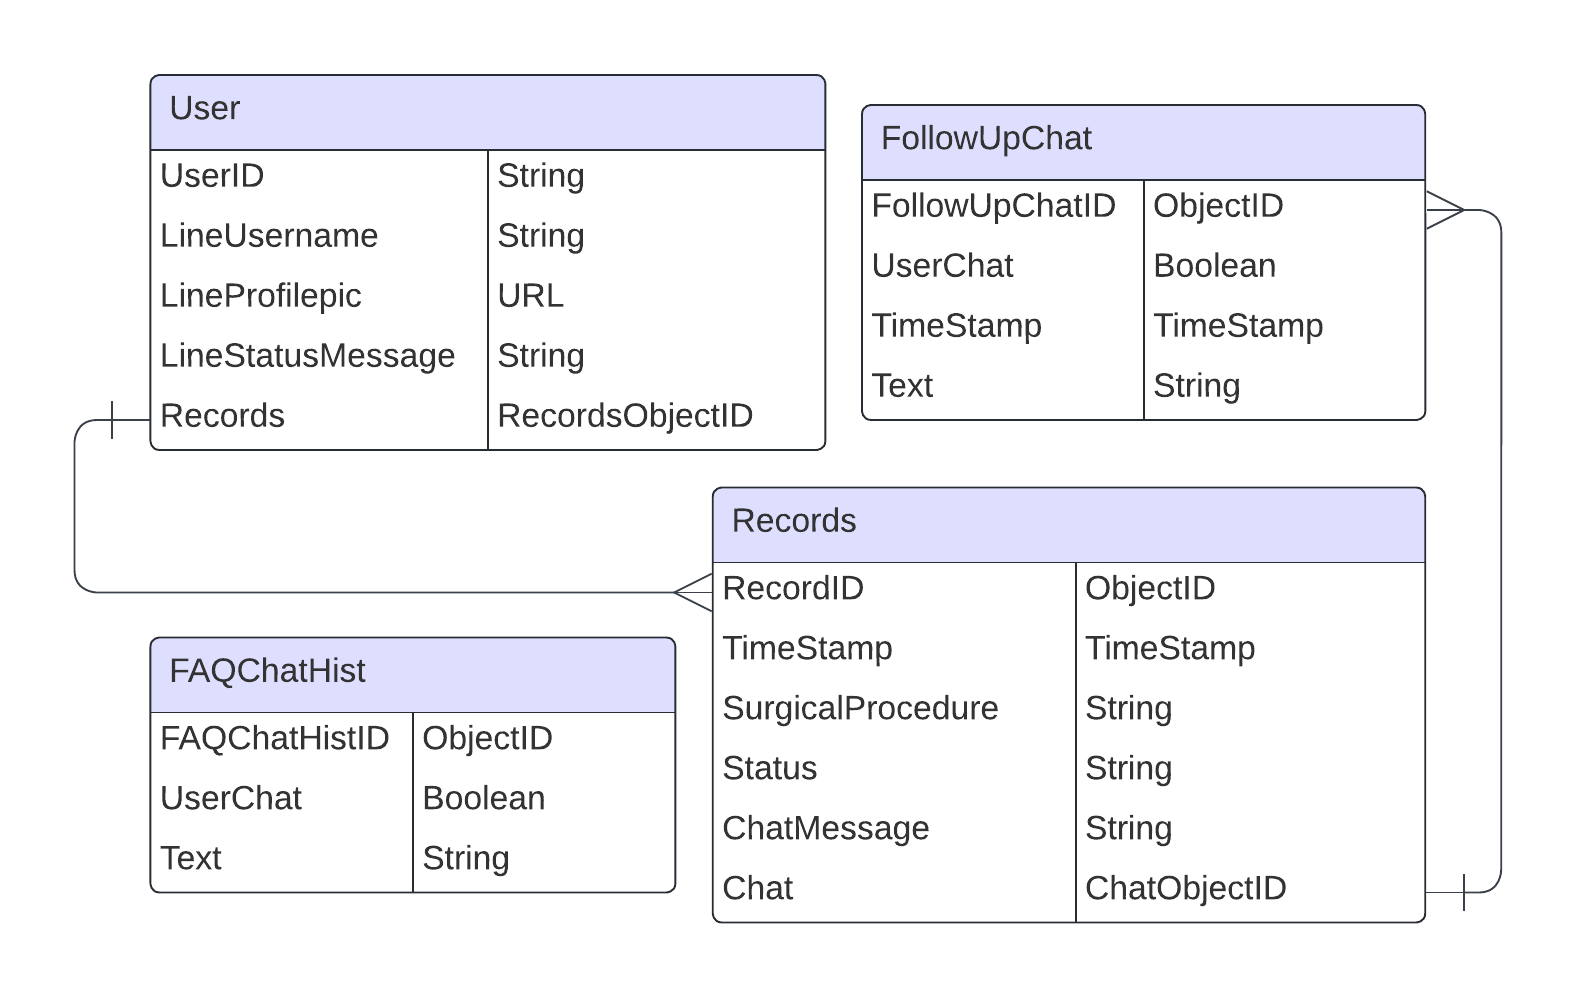
\includegraphics[width=.35\textwidth]{Image/ER.png}}
      \caption{ER-Diagram}\label{fig:ER}
      \begin{itemize}
        \item[] 1. Figure 3.10 shows the basic database design necessary for storing registered users in our application. The database comprises a total of 4 objectsUser Object: This object includes userID, LineUsername, LineProfilepic, and LineEmail, all linked to the Line profile. Additionally, the User Object contains lists of Records Object.
        \item[] 2. Records Object: It encompasses RecordID, TimeStamp, SurgicalProcedure, Status, ChatMessage and FollowUpChat Object. The RecordID is linked to the User object and FollowUpChat Object.
        \item[] 3. FollowUpChat Object: This object contains FollowUpID, Title, TimeStamp, Chat, and ChatResult. The FollowUpID is linked to the Records object in a one-to-many relation.
        \item[] 4. FAQChatHist Object: It includes FAQChatHistID, UserChat, Text, User and ChatTime which are kept for further training our model.
        \item[] These objects and their interconnections form the basic structure of our database for storing user-related information, their records, follow-ups, and chat interactions.
      \end{itemize}
    \end{figure}
  \section{User Interface}
    \subsection{Home Page}
    \begin{figure}[!h]
      \centering
      \begin{minipage}{.5\textwidth}
        \centering
        \fbox{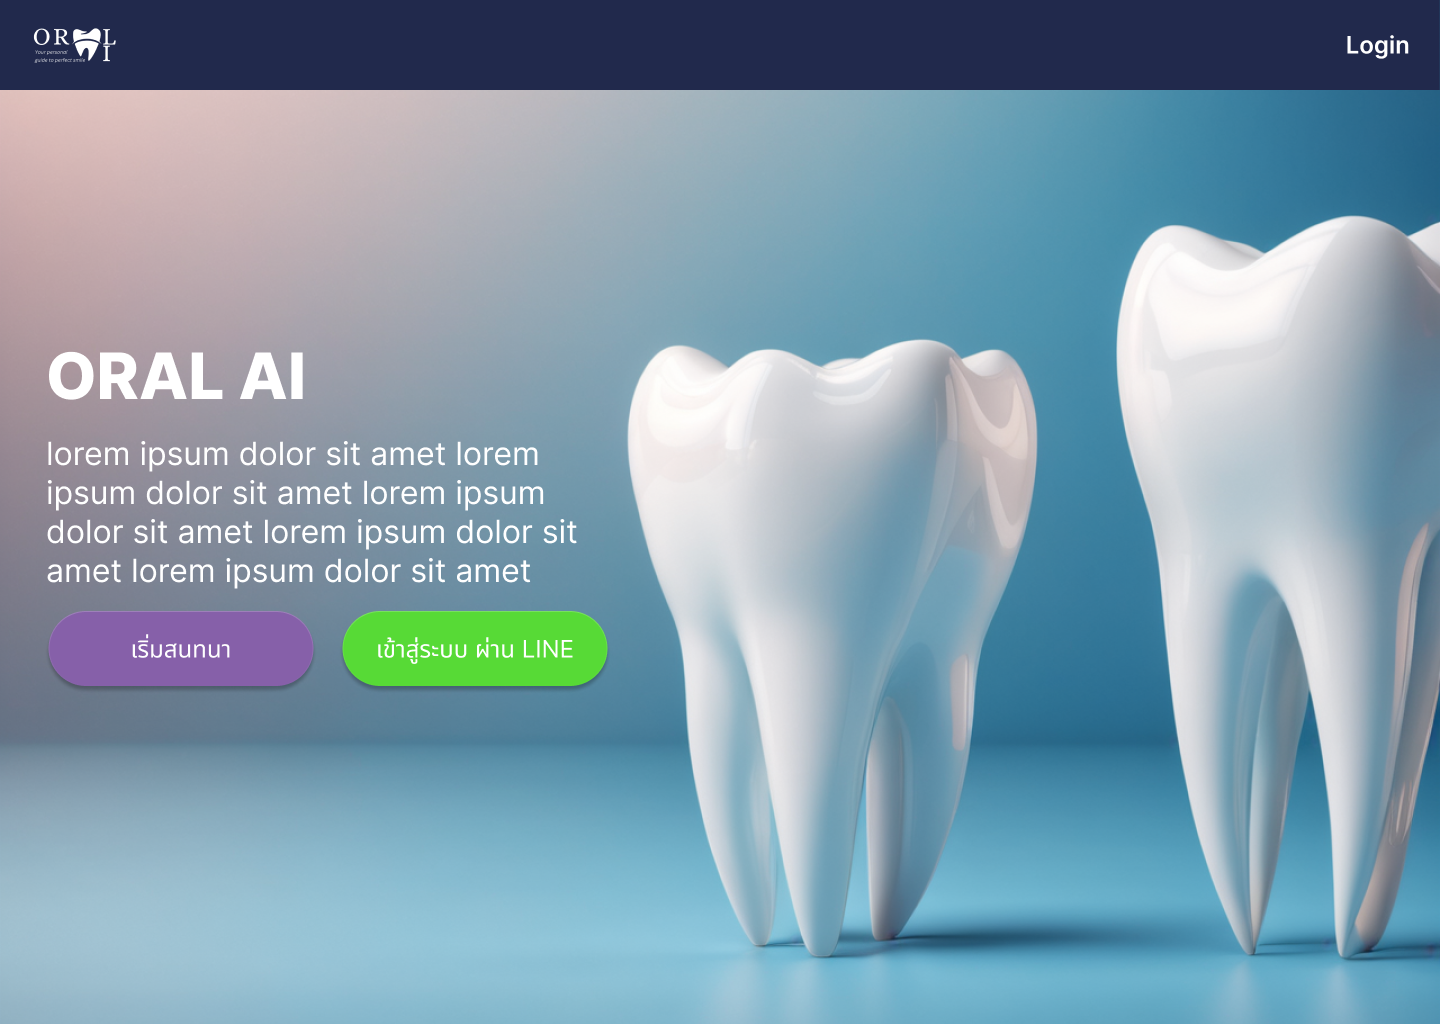
\includegraphics[width=.7\linewidth]{Image/Desk_Home.png}}
      \end{minipage}%
      \begin{minipage}{.3\textwidth}
        \centering
        \fbox{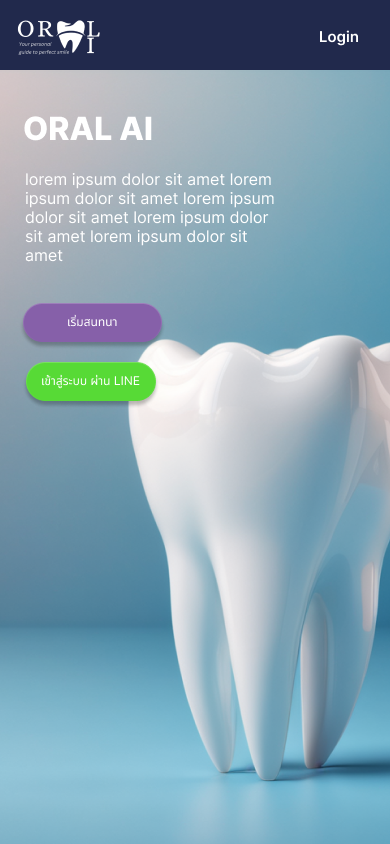
\includegraphics[width=.4\linewidth]{Image/Mob_Home.png}}
      \end{minipage}
      \caption{Website home page (Desktop and mobile respectively)}\label{fig:HomePage}
      \begin{flushleft}
        \qquad Figure 3.11 represents the home page of our web application. This page provides a brief description of our website and features two primary buttons: “Start Chatting” and “Login by Line”.
        \begin{itemize}
          \item The “Start Chatting” button redirect users to the question answering page, facilitating interaction with the chatbot for inquiries.
          \item “Login by Line” directs users to the Line login page, allowing them to log into the platform using their Line account credentials.
        \end{itemize}
      \end{flushleft}
    \end{figure}
    \newpage

    \subsection{Follow-Up page}
      \begin{figure}[!h]
        \centering
        \fbox{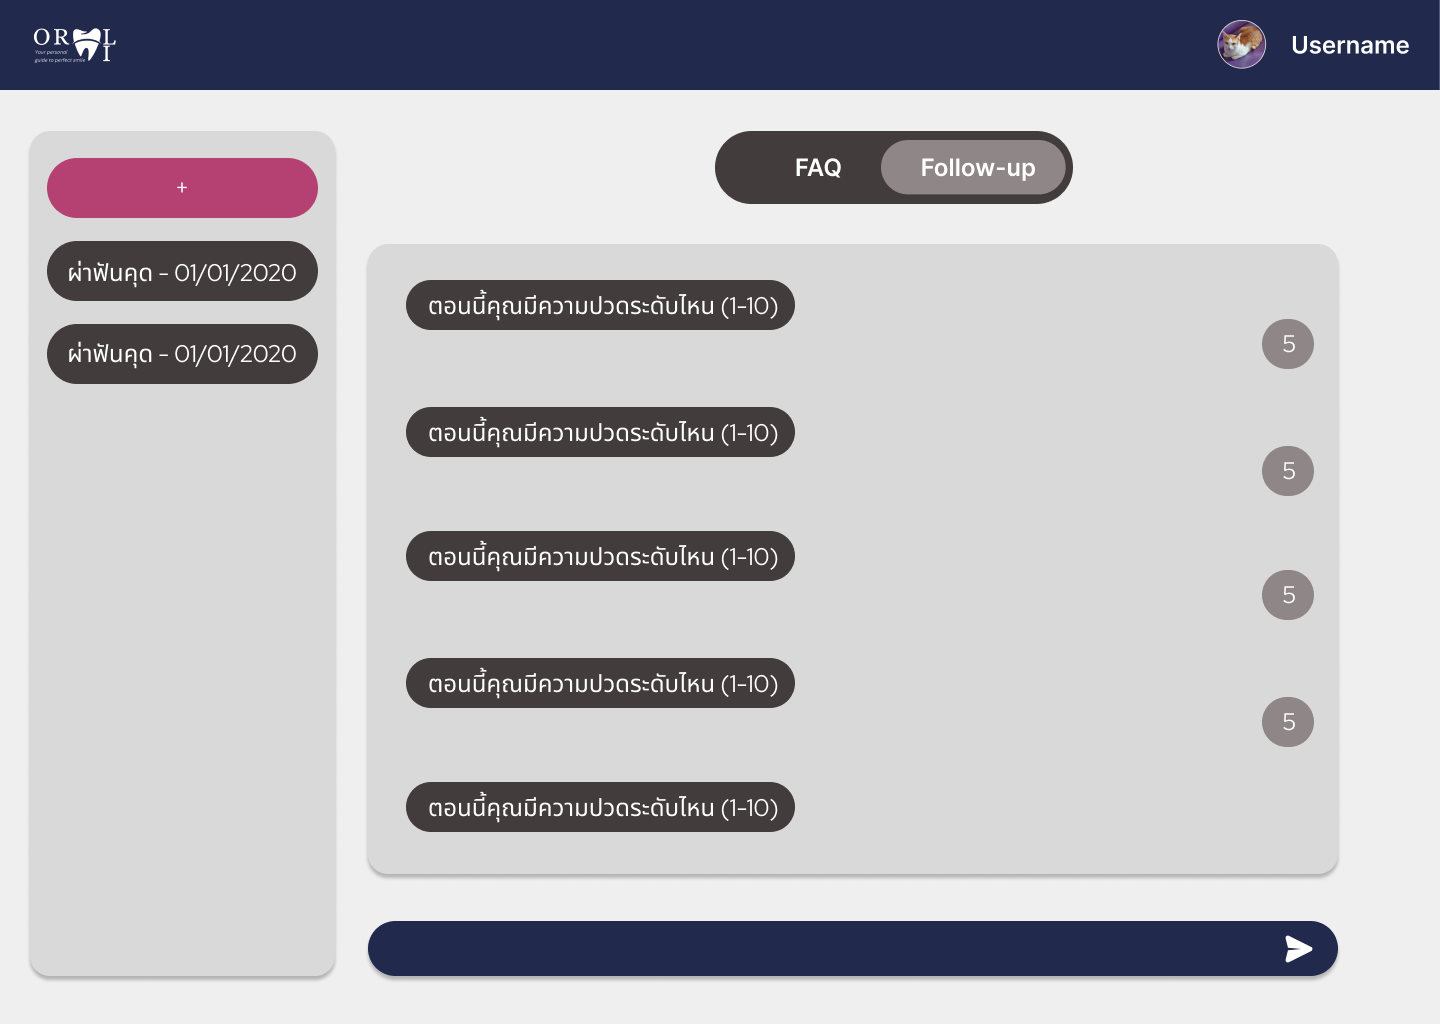
\includegraphics[width=.35\textwidth]{Image/Desk_Follow.png}}
        \caption{Desktop Follow-Up page}\label{fig:Desk_Follow}
        \begin{flushleft}
          \qquad Figure 3.12 showcases the Follow-Up page of the web application specifically designed for the desktop use. The layout consists of several key components: \par
          \begin{itemize}
            \item Case History: Positioned on the left side, this section displays the user’s case history. Users can click on specific cases to view their follow-up chat history. The top button allow user to add new case.
            \item Chat Box: Positioned in the middle, this area hosts the ongoing chat conversation. User can engage in follow-up discussions within this section. 
            \item Input Textbox: Positioned beneath the chat box, this textbox enables users to input their responses during the follow-up conversation. 
            \item Switch Bar: Located at the top of the chat box, this bar facilitates the transition between the FAQ and Follow-up features.
          \end{itemize}
        \end{flushleft}
      \end{figure}

    \begin{figure}[!h]
      \centering
      \begin{minipage}{.15\textwidth}
        \centering
        \fbox{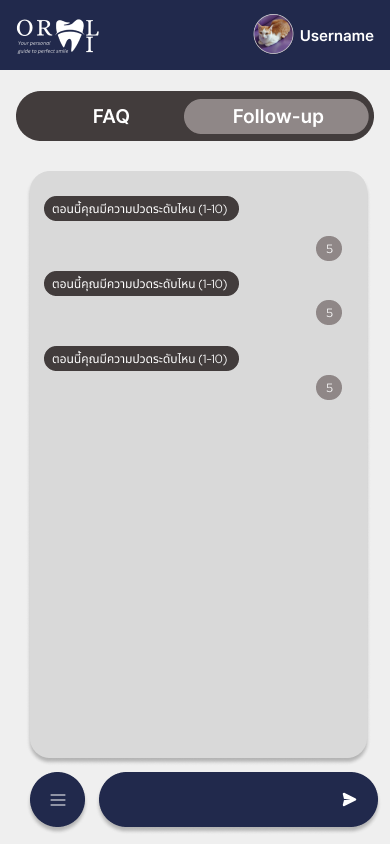
\includegraphics[width=.7\linewidth]{Image/Mob_Follow_1.png}}
      \end{minipage}%
      \begin{minipage}{.15\textwidth}
        \centering
        \fbox{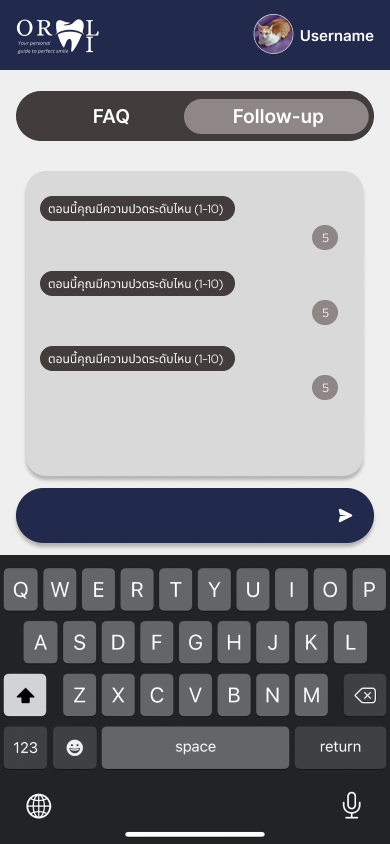
\includegraphics[width=.7\linewidth]{Image/Mob_Follow_2.png}}
      \end{minipage}%
      \begin{minipage}{.15\textwidth}
        \centering
        \fbox{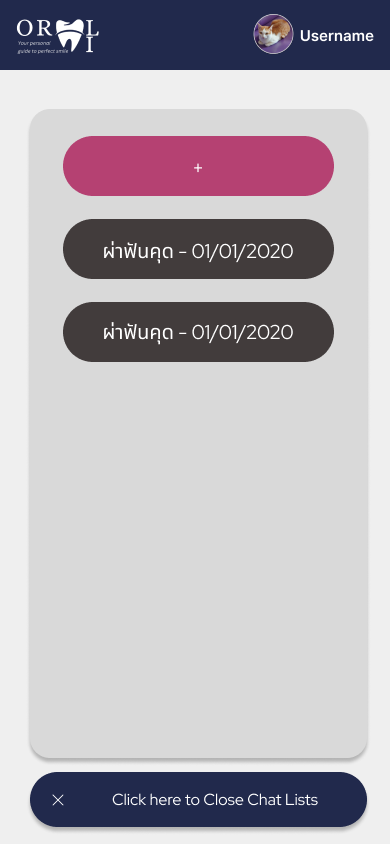
\includegraphics[width=.7\linewidth]{Image/Mob_Follow_3.png}}
      \end{minipage}
      \caption{Mobile Follow-Up page}\label{fig:Mob_Follow}
      \begin{flushleft}
        \qquad Figure 3.13 display the mobile version of the Follow-Up page in various scenarios:  \par
        \begin{itemize}
          \item Normal Page (Left): This view represents the default appearance of the Follow-Up page on a mobile device.
          \item Keyboard Usage (Center): When the keyboard is engaged, this display is centered on the chat or input area.
          \item Hamburger Button Pressed (Right): Upon pressing the hamburger button, the keyboard input is dismissed, replaced by a long-closed button. This button allows users to return to the Follow-Up page. The top button allow user to add new case.
        \end{itemize}
      \end{flushleft}
    \end{figure}

    \subsection{FAQ page}
    \begin{figure}[!h]
      \centering
      \fbox{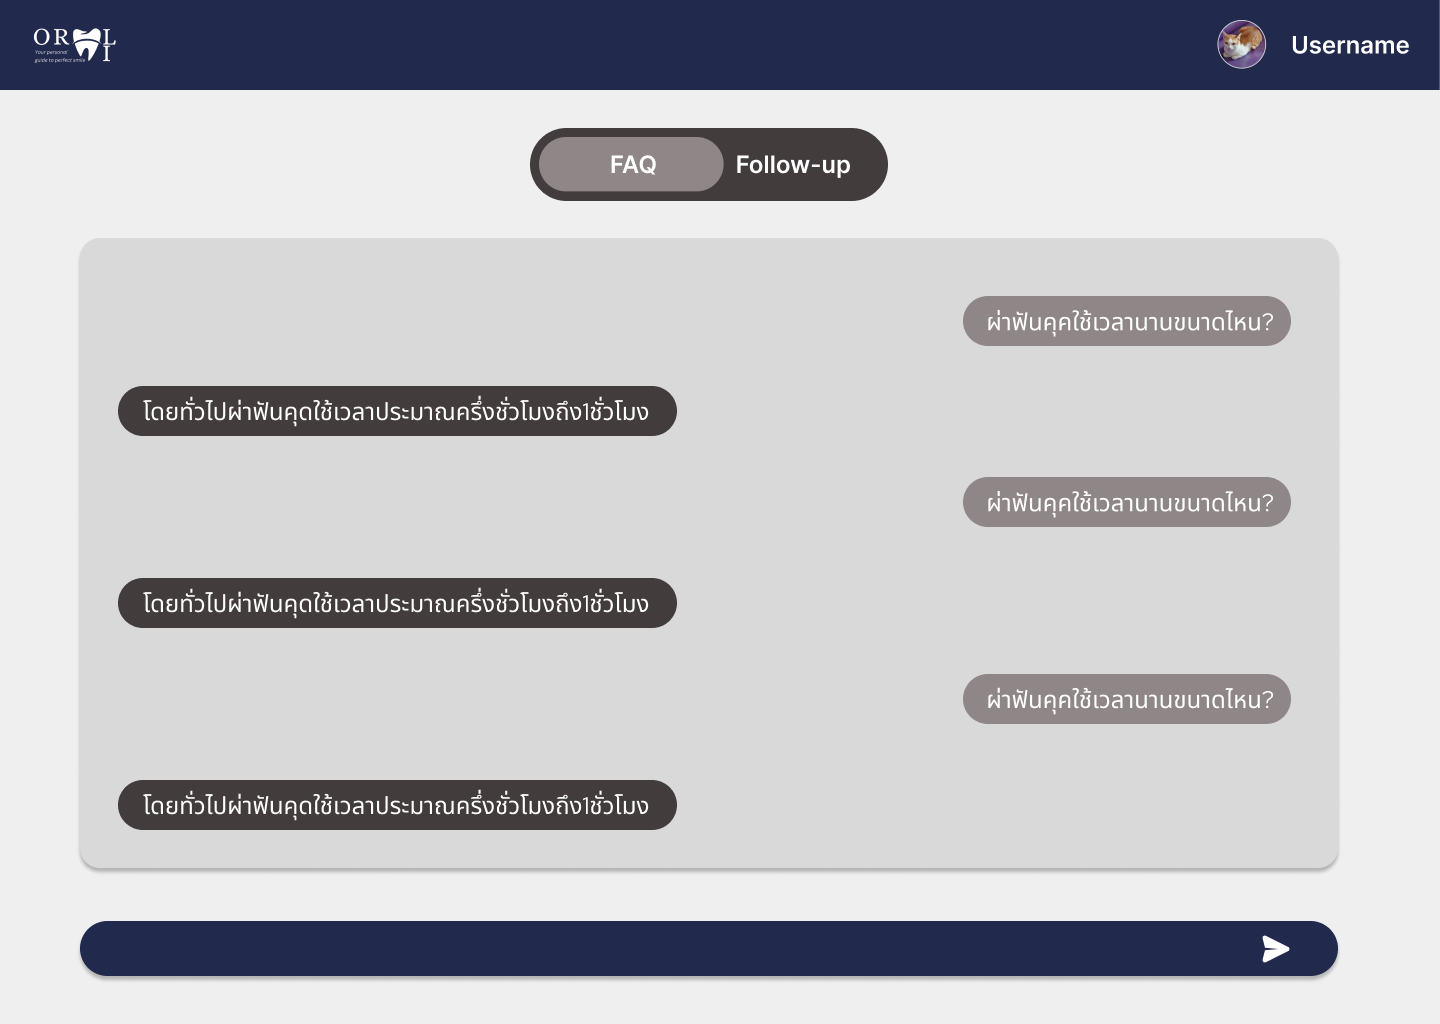
\includegraphics[width=.4\textwidth]{Image/Desk_FAQ.png}}
      \caption{Desktop Question Answering page}\label{fig:Desk_FAQ}
      \begin{flushleft}
        \qquad Figure 3.14 depicts the desktop version of the Question Answering page within the web application. The page features a central chat box facilitating user-system interaction for addressing queries, accompanied by an input textbox positioned at the bottom. Additionally, a switch bar located atop the chat box facilitates switching between the FAQ and Follow-up features. \par
      \end{flushleft}
    \end{figure}
    \begin{figure}[!h]
      \centering
      \begin{minipage}{.3\textwidth}
        \centering
        \fbox{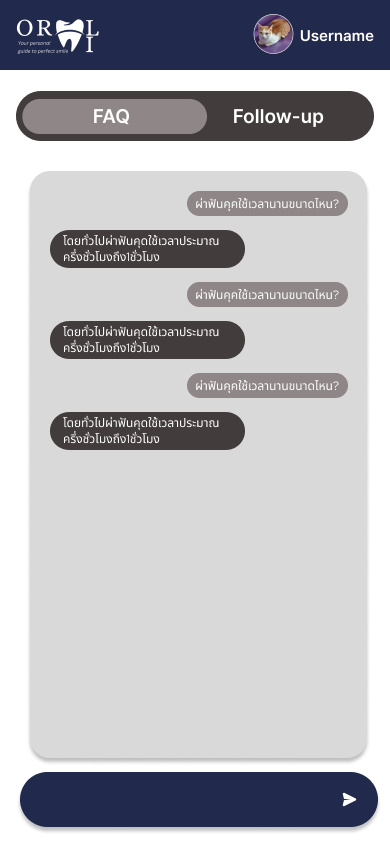
\includegraphics[width=.6\linewidth]{Image/Mob_FAQ_1.png}}
      \end{minipage}%
      \begin{minipage}{.3\textwidth}
        \centering
        \fbox{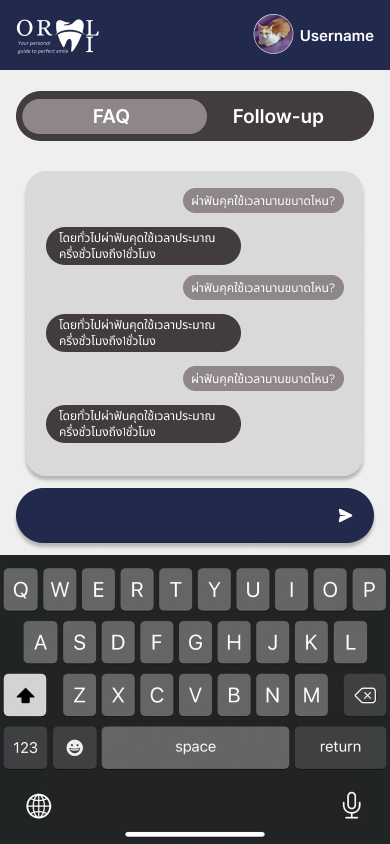
\includegraphics[width=.6\linewidth]{Image/Mob_FAQ_2.png}}
      \end{minipage}%
      \caption{Mobile Question Answering page}\label{fig:Mobile Question Answering page}
      \begin{flushleft}
        \qquad Figure 3.15 illustrates the Question Answering page of the web application on mobile. On the left is its normal page view, and on the right is the interface when the keyboard is in use. \par
      \end{flushleft}
    \end{figure}
\newpage
    \subsection{Patient Info page}
    \begin{figure}[!h]
      \centering
      \begin{minipage}{.7\textwidth}
        \centering
        \fbox{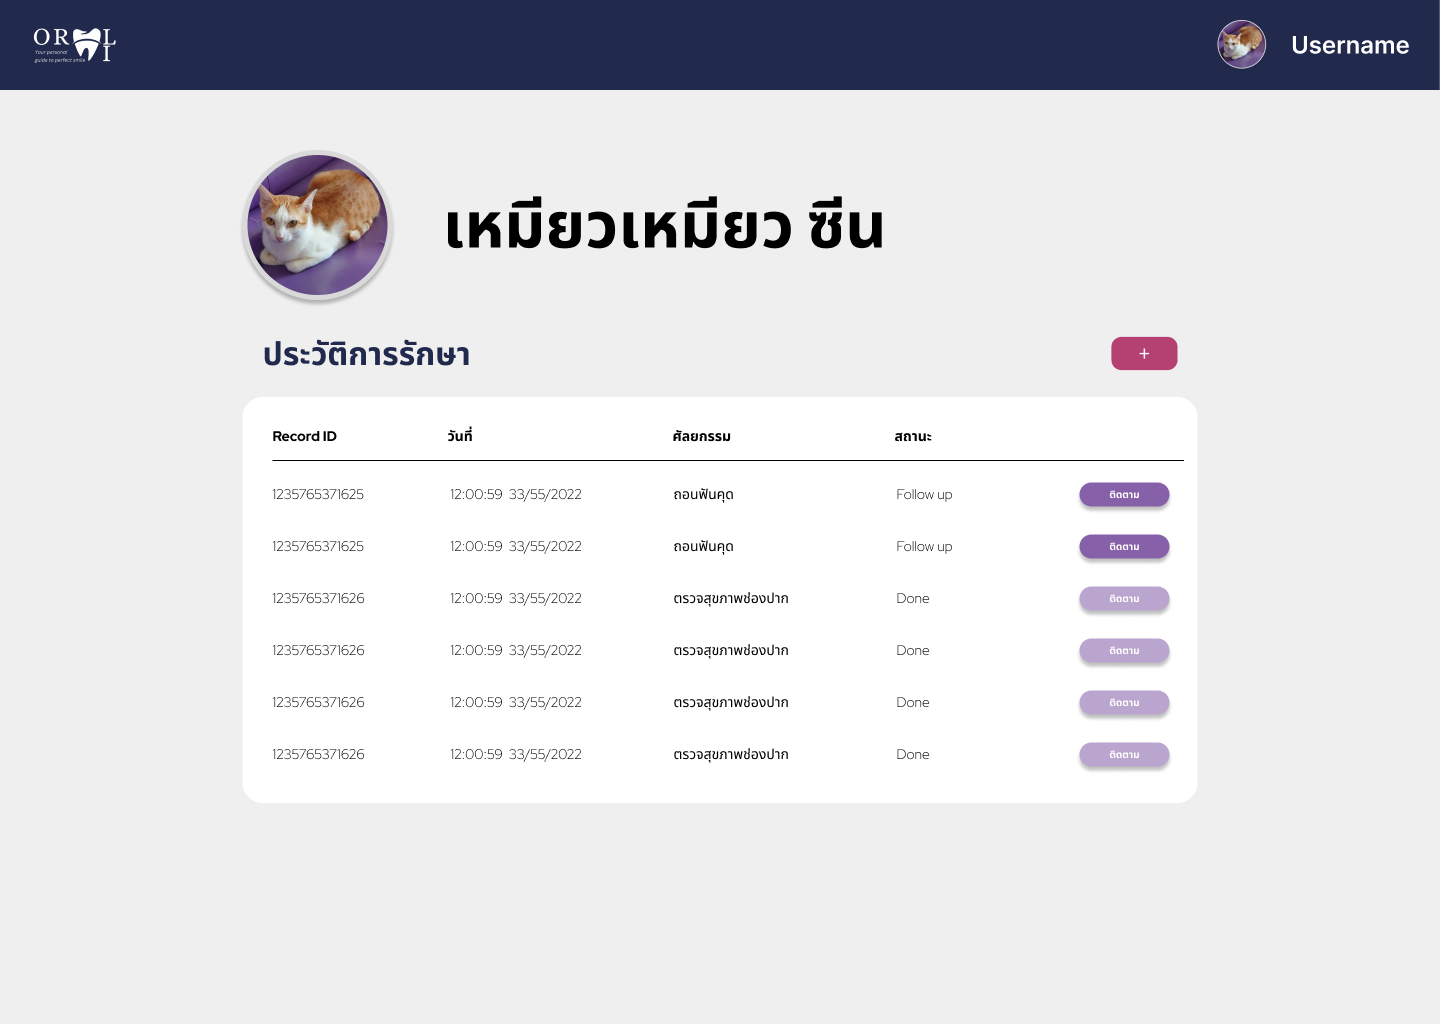
\includegraphics[width=.7\linewidth]{Image/Desk_Info.png}}
      \end{minipage}%
      \begin{minipage}{.25\textwidth}
        \centering
        \fbox{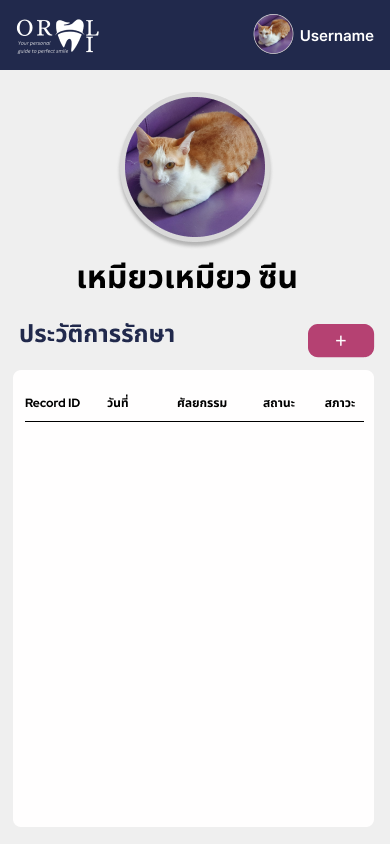
\includegraphics[width=.6\linewidth]{Image/Mob_Info.png}}
      \end{minipage}
      \caption{Patient Information page (Desktop and mobile respectively)}\label{fig:Patient Information page}
      \begin{flushleft}
        \qquad Figure 3.16 represents the Patient Information page within the web application, displaying the comprehensive oral medical history registered by the patient. The records display the Record ID, Timestamp, Surgical Procedures type, status, and associated conditions. \par
      \end{flushleft}
    \end{figure}
    \subsection{Line official page}
    \begin{figure}[!h]
      \centering
      \begin{minipage}{.3\textwidth}
        \centering
        \fbox{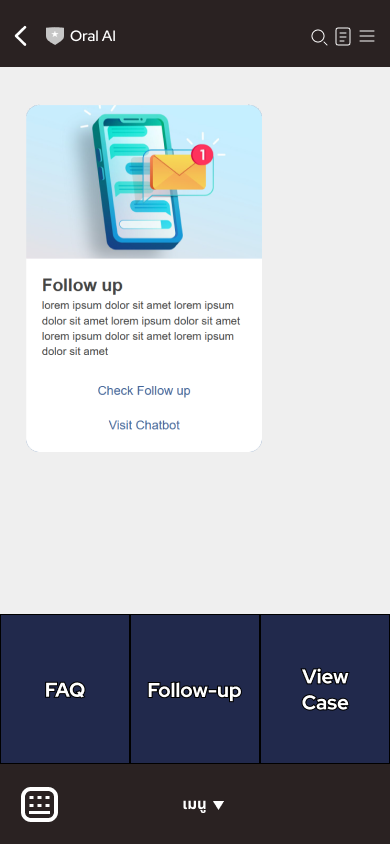
\includegraphics[width=.6\linewidth]{Image/Line_1.png}}
      \end{minipage}%
      \begin{minipage}{.3\textwidth}
        \centering
        \fbox{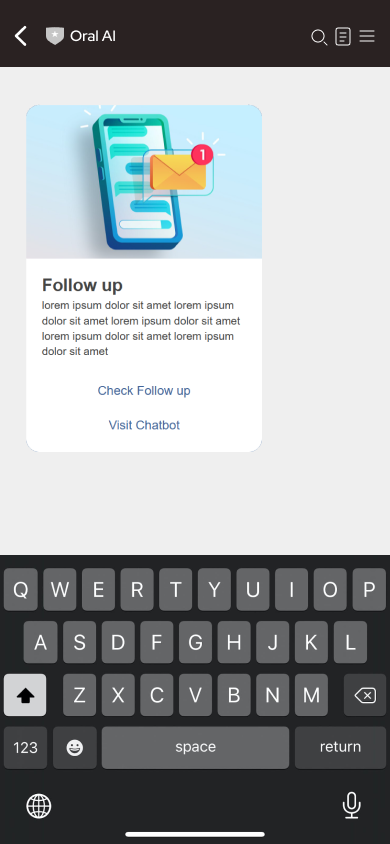
\includegraphics[width=.6\linewidth]{Image/Line_2.png}}
      \end{minipage}%
    
      \caption{Line Login Page}\label{fig:Line Login Page}
      \begin{flushleft}
        \qquad Figure 3.17 showcases the layout of the Line Official page, acting as the central notification hub within the application. The FAQ button directs users to the question answer website, the Follow-up button leads to the follow-up page on the website, and the View Case navigates users to the patient information page. \par
      \end{flushleft}
    \end{figure}
\newpage
  \section{Evaluation Plan}
    \subsection{User Evaluation}
      \qquad Upon the completion of platform development aligned with our objectives, we aim to conduct testing and gather user feedback. Our assessment will encompass overall satisfaction, usability, user experience, and suggestions for enhancements. Subsequently, the collected data will undergo thorough analysis to evaluate the application. \par
    \subsection{Application Evaluation}
      \qquad For assessing critical components, our focus will center on two key metrics. First, Response Latency will be closely monitored to gauge the chatbot’s speed in addressing user queries. Moreover, the accuracy in providing precise and correct responses to dental inquiries will ensures the chatbot's proficiency in delivering accurate information. \par


\chapter{EXPERIMENTAL RESULTS}
  \section{Dental Frequently Asked Question Collection}
    \qquad To ensure the project’s ability to address user queries effectively, we have gathered a list of frequently asked questions about the four specified surgeries. Surveys were conducted, and experts were consulted to guarantee accurate and appropriate answers. This section contains the questionnaire and its corresponding results. \par
    \subsection{Collection Process}
      \qquad The questions were collected using Google Forms. The provided questionnaire aimed to cover a broad range of opinions and concerns regarding dental health and medical treatments. Questions within the questionnaire included inquiries about past treatments or surgeries (\textthai{คุณเคยผ่านการรักษาหรือการผ่าตัดไหนมาแล้วบ้าง}), reasons for undergoing treatment/surgery (\textthai{สาเหตุที่คุณเข้ารับการรักษา/ผ่าตัด}), commonly encountered or doubtful inquiries regarding the aforementioned diseases, treatments, or surgeries (\textthai{คำถามที่มักจะเจอหรือสงสัยเกี่ยวกับโรคและการรักษา/ผ่าตัดข้างต้น}), and questions often raised post-treatment/surgery (\textthai{คำถามที่มักสงสัยหลังจากที่ได้รับการรักษา/ผ่าตัด}). \par
      \begin{figure}[!h]
        \centering
        \fbox{
\includegraphics[width=.5\textwidth]{Image/Survey_1.png}}
        \caption{First page of the questionnaire}\label{fig:Survey_1}
      \end{figure}
      \begin{figure}[!h]
        \centering
        \fbox{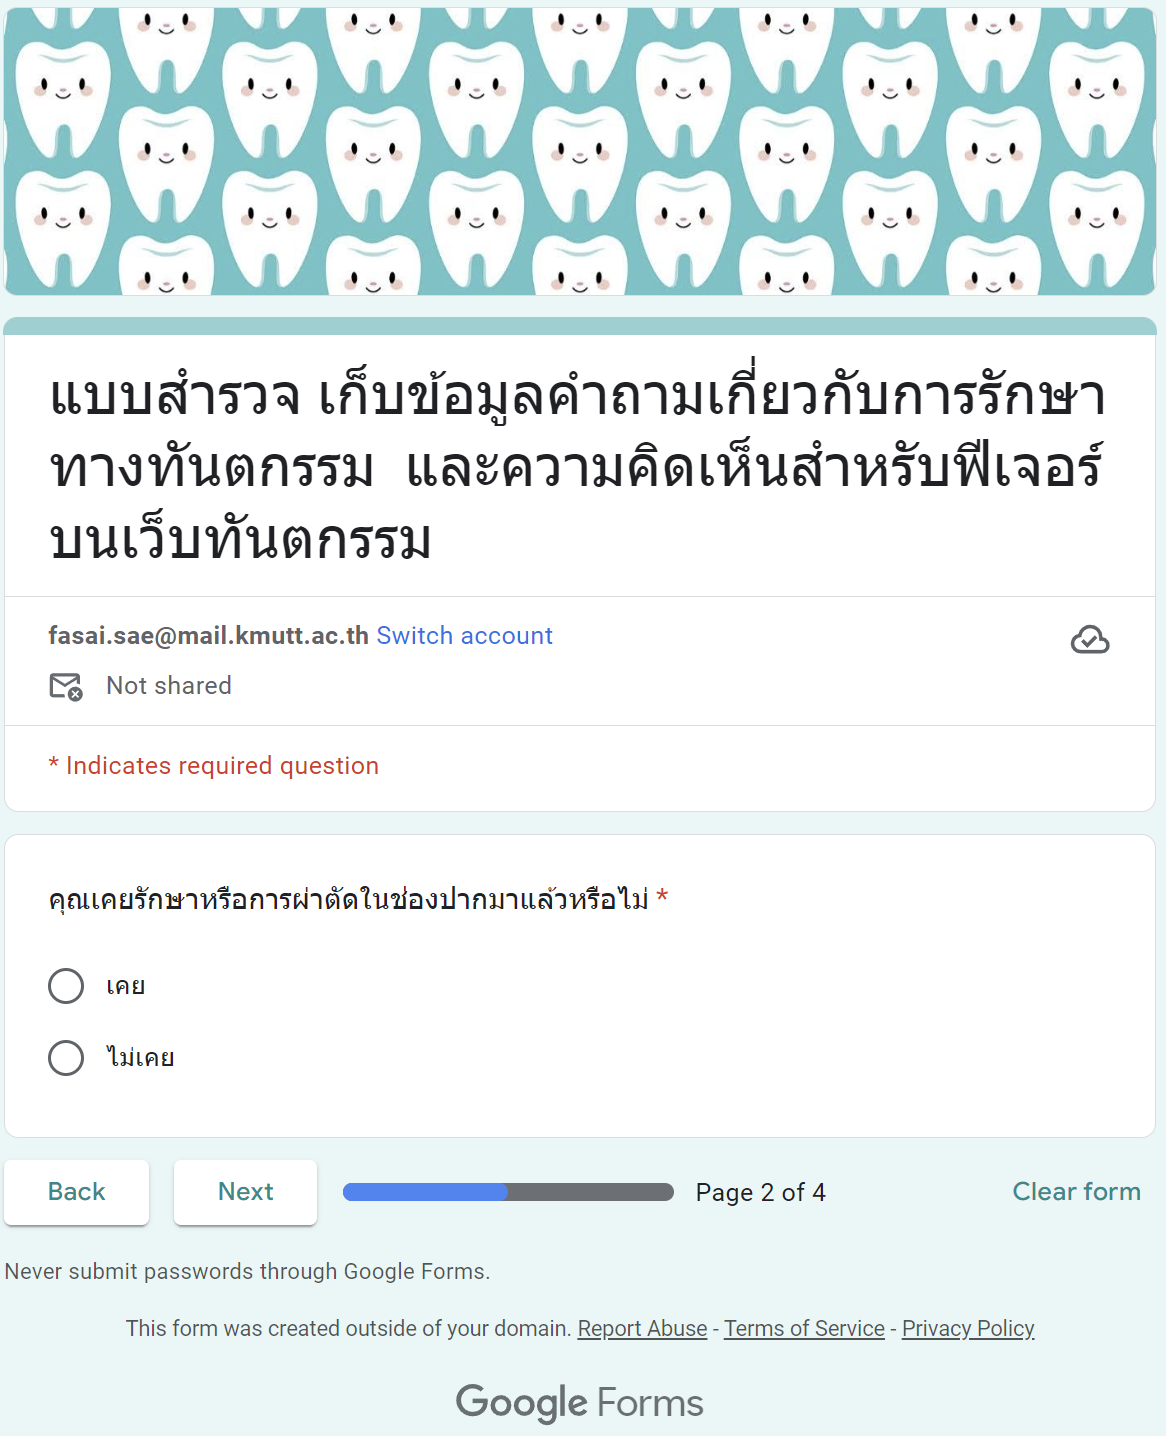
\includegraphics[width=.37\textwidth]{Image/Survey_2.png}}
        \caption{Second page of the questionnaire}\label{fig:Survey_2}
      \end{figure}
      \begin{figure}[!h]
        \centering
        \fbox{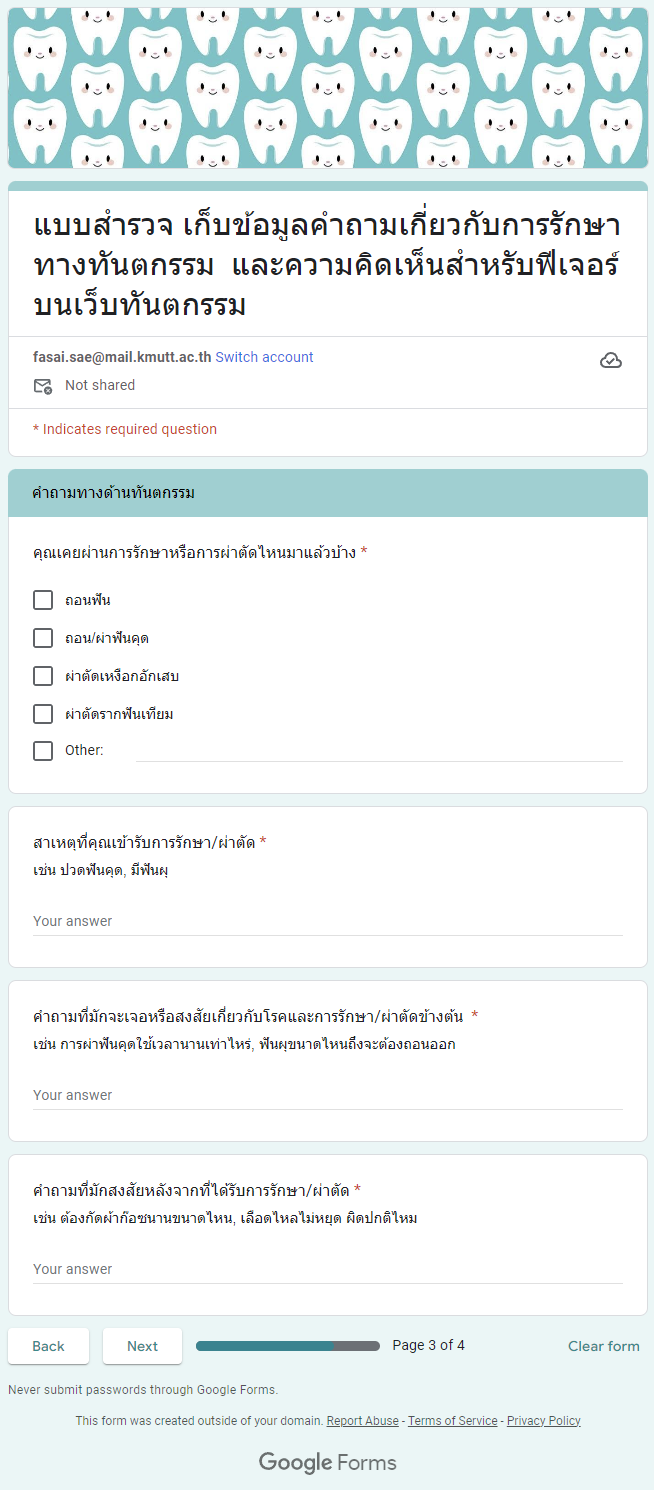
\includegraphics[width=.4\textwidth]{Image/Survey_3.png}}
        \caption{Third page of the questionnaire}\label{fig:Survey_3}
      \end{figure}
      \begin{figure}[!h]
        \centering
        \fbox{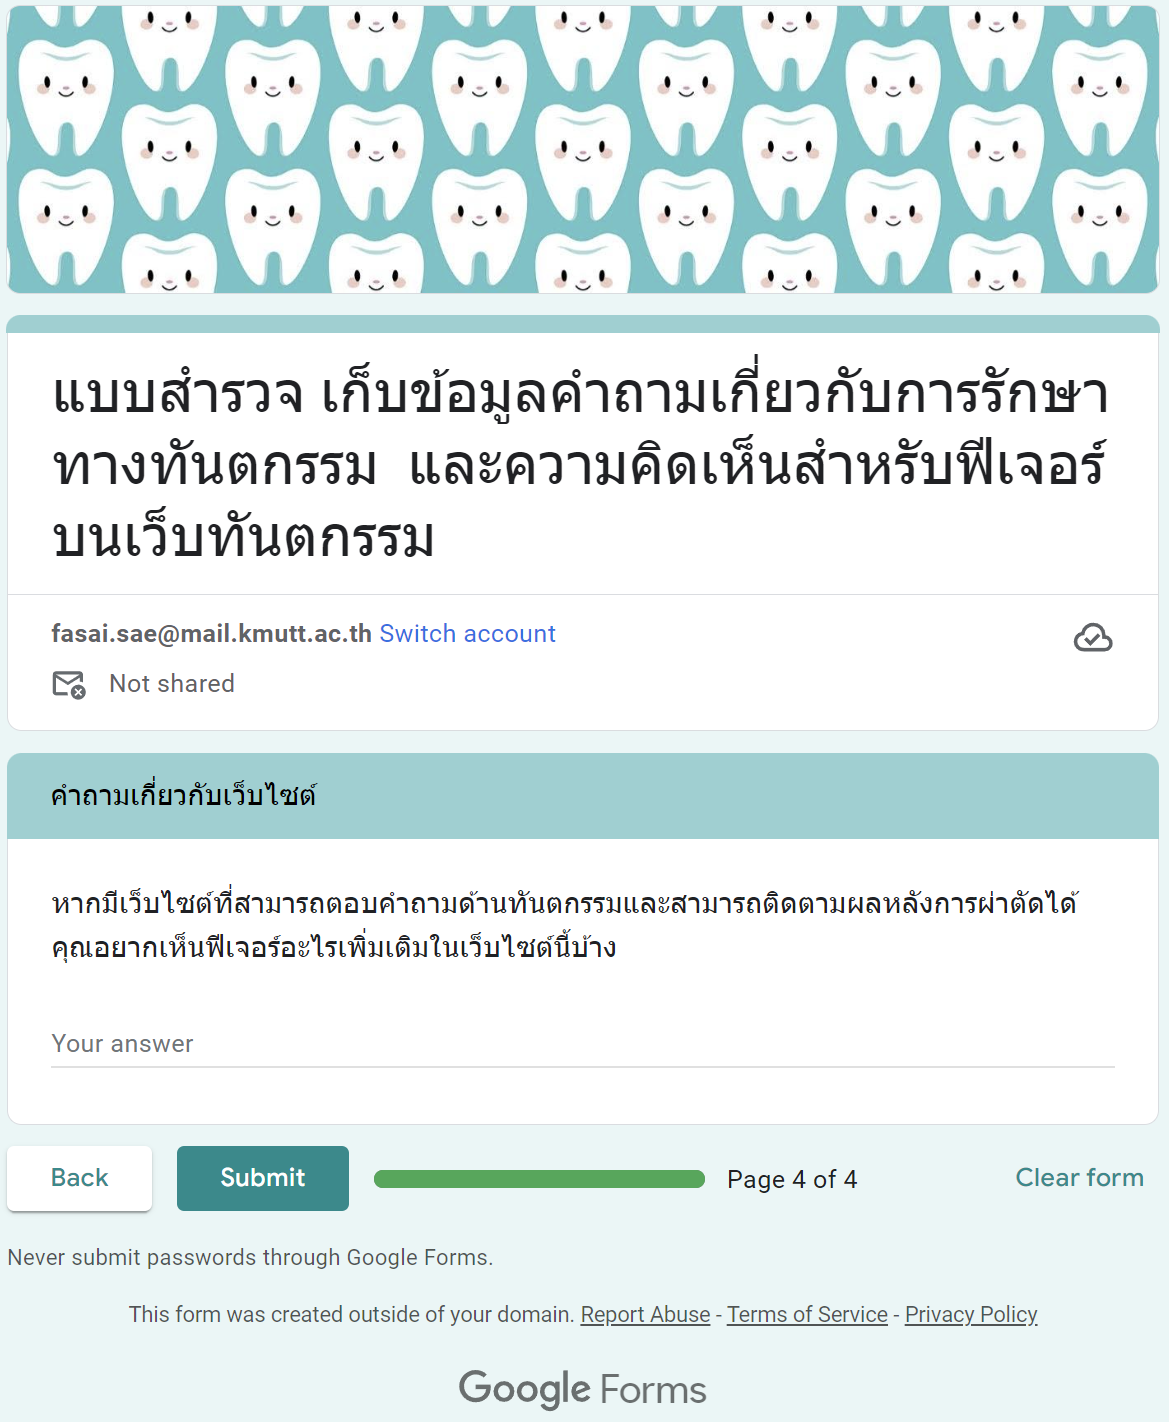
\includegraphics[width=.4\textwidth]{Image/Survey_4.png}}
        \caption{Fourth page of the questionnaire}\label{fig:Survey_4}
      \end{figure}
      \FloatBarrier{}
    \subsection{Results}
      \begin{figure}[!h]
        \centering
        \fbox{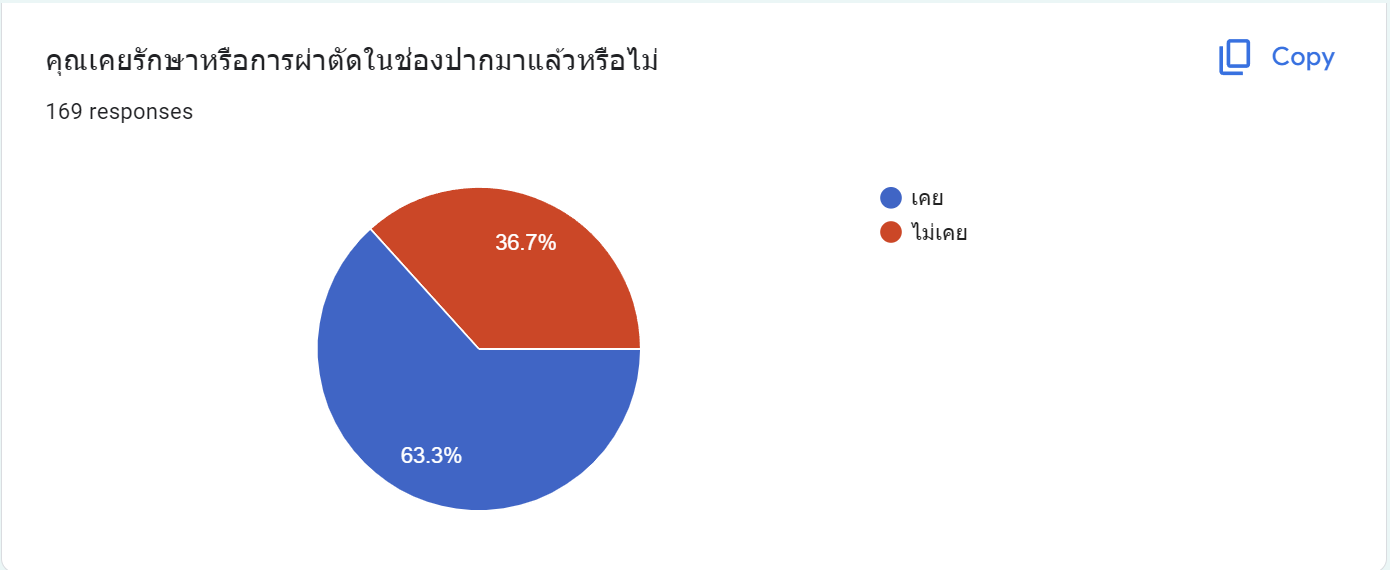
\includegraphics[width=.6\textwidth]{Image/Result_1.png}}
        \caption{Pie chart of Distribution of Oral Surgery Experience}\label{fig:Result_1}
      \end{figure}
      \begin{figure}[!h]
        \centering
        \fbox{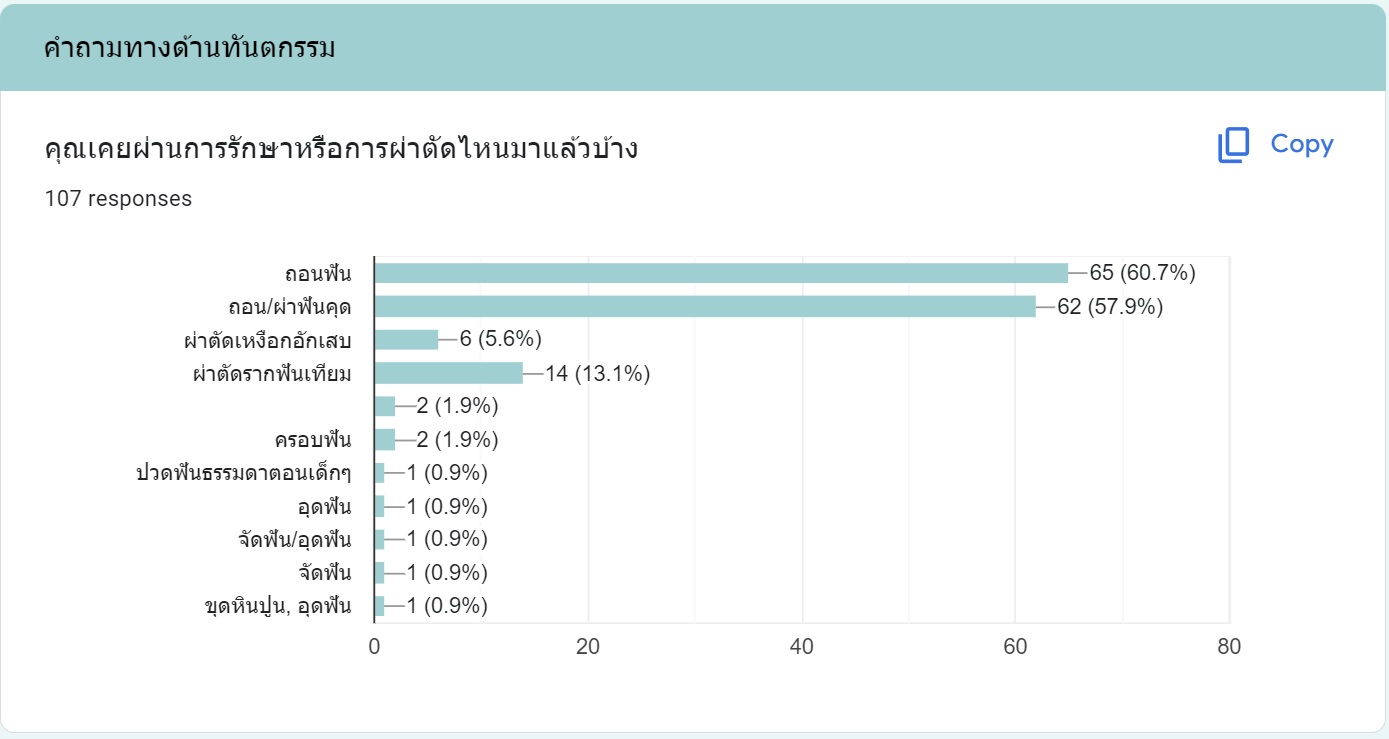
\includegraphics[width=.6\textwidth]{Image/Result_2.png}}
        \caption{Respondent’s Oral Surgeries Experience}\label{fig:Result_2}
      \end{figure}
      \begin{figure}[!h]
        \centering
        \fbox{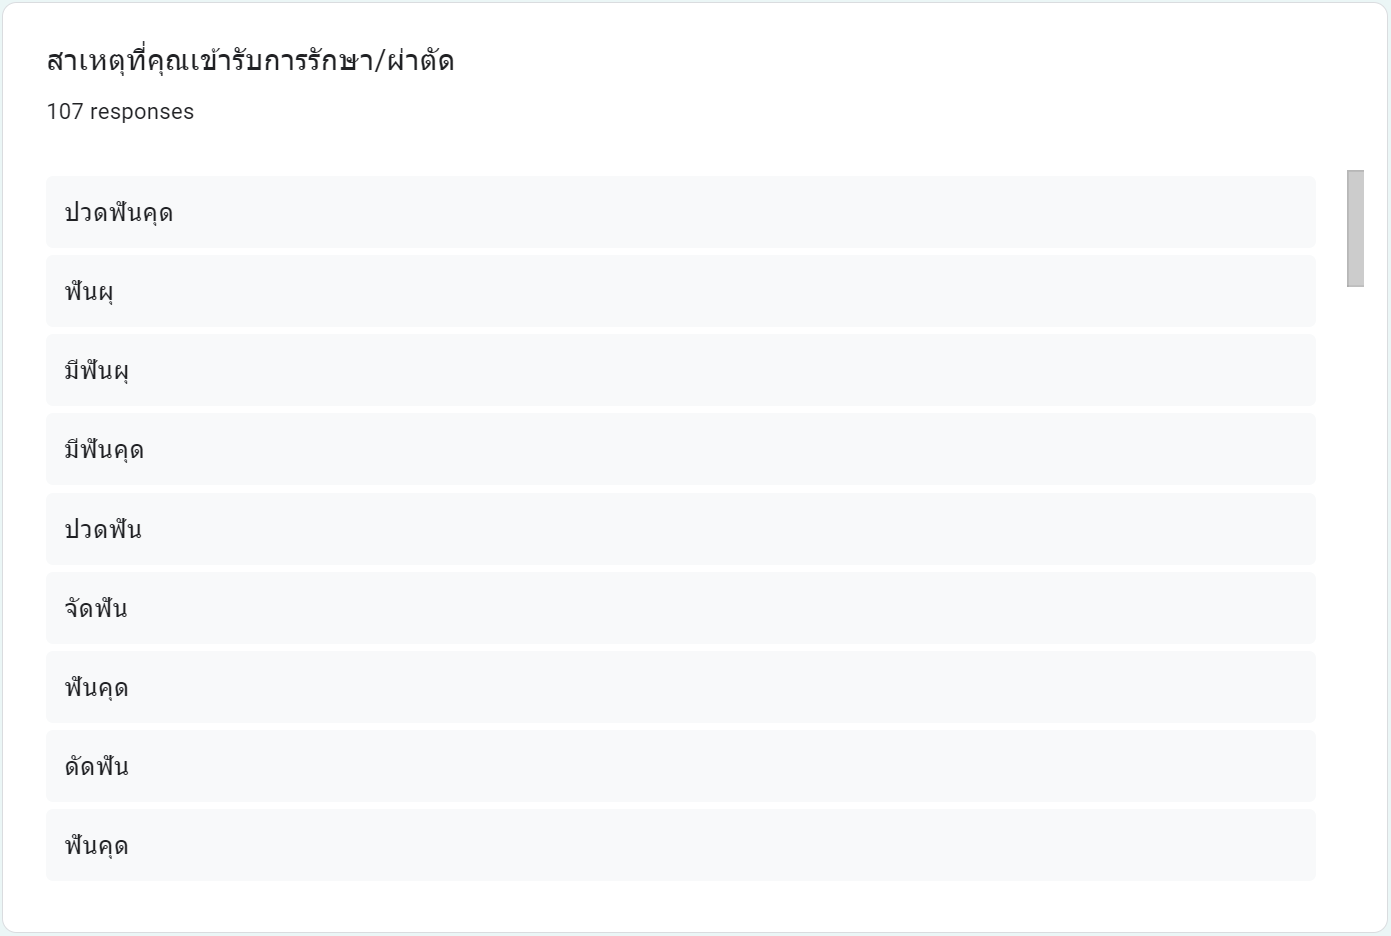
\includegraphics[width=.6\textwidth]{Image/Result_3.png}}
        \caption{Reason the Respondent Attend the Treatment}\label{fig:Result_3}
      \end{figure}
      \begin{figure}[!h]
        \centering
        \fbox{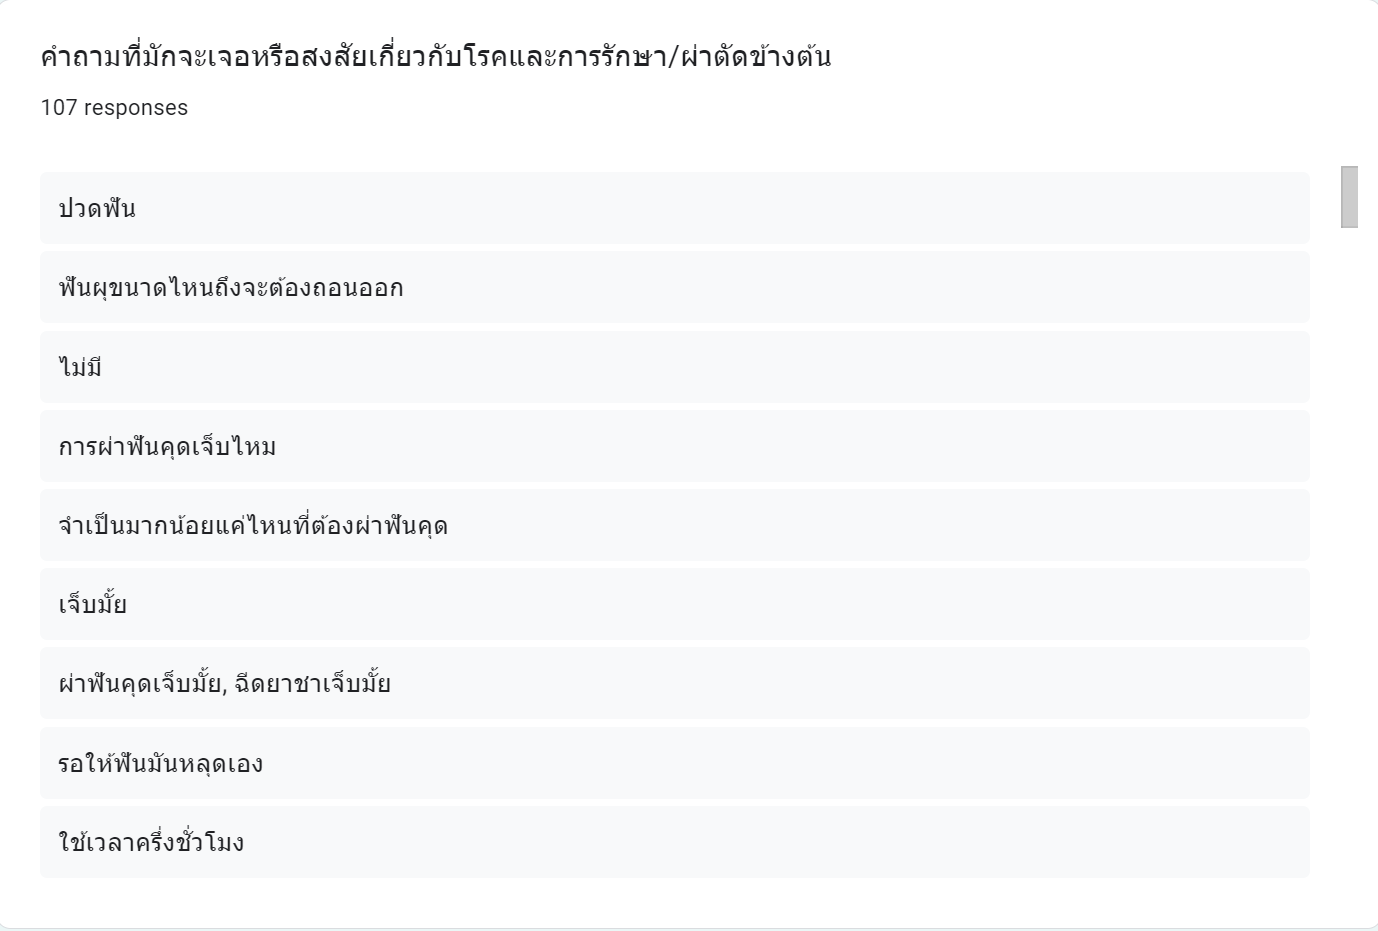
\includegraphics[width=.6\textwidth]{Image/Result_4.png}}
        \caption{Common Questions and Concerns About Surgeries and Treatment}\label{fig:Result_4}
      \end{figure}
      \begin{figure}[!h]
        \centering
        \fbox{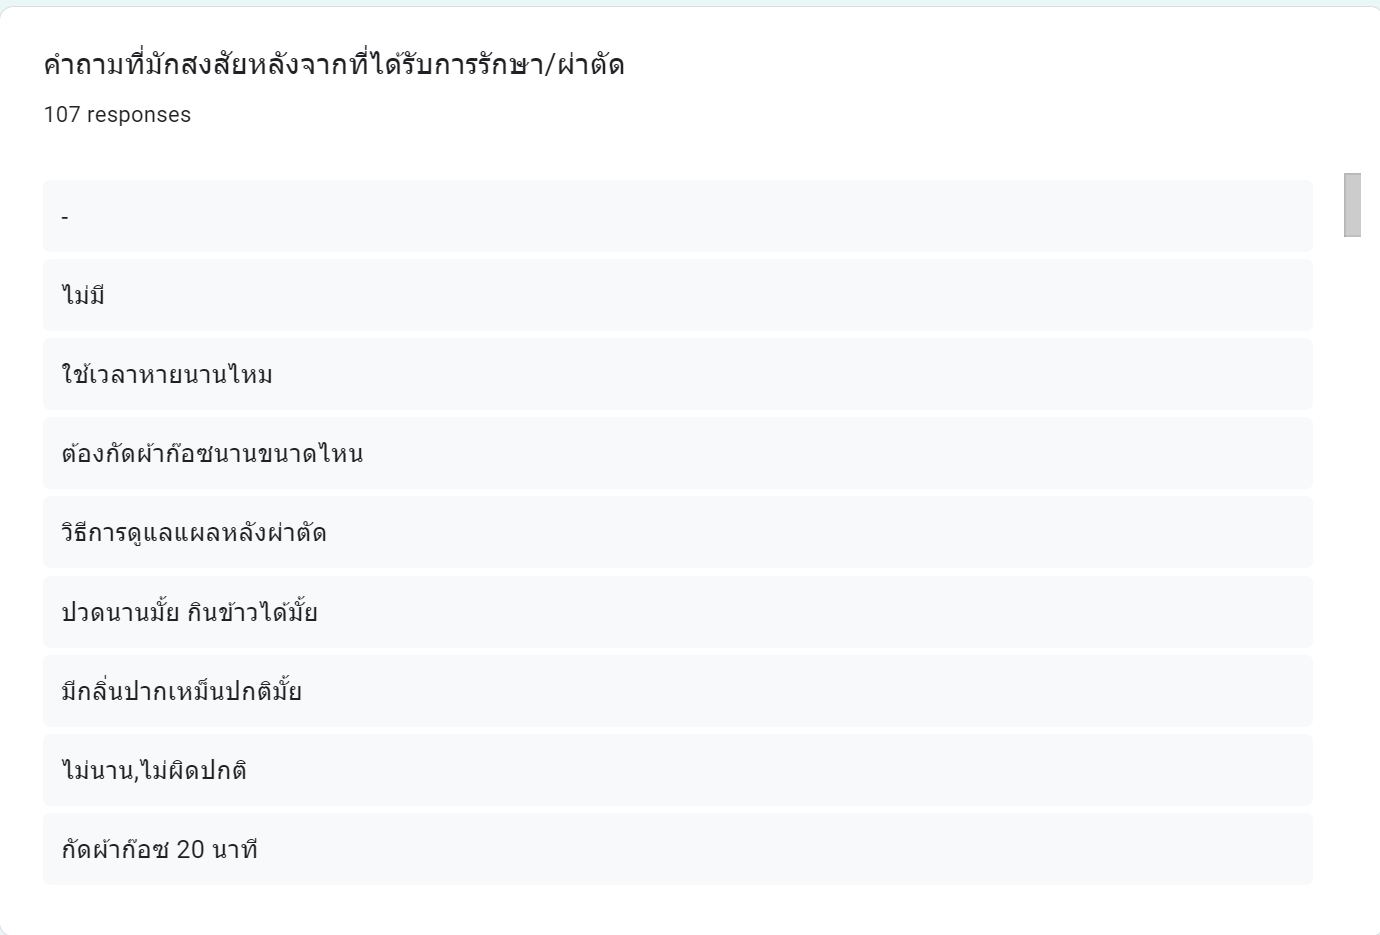
\includegraphics[width=.6\textwidth]{Image/Result_5.png}}
        \caption{Post-Treatment Frequently Asked Questions}\label{fig:Result_5}
      \end{figure}
      \begin{figure}[!h]
        \centering
        \fbox{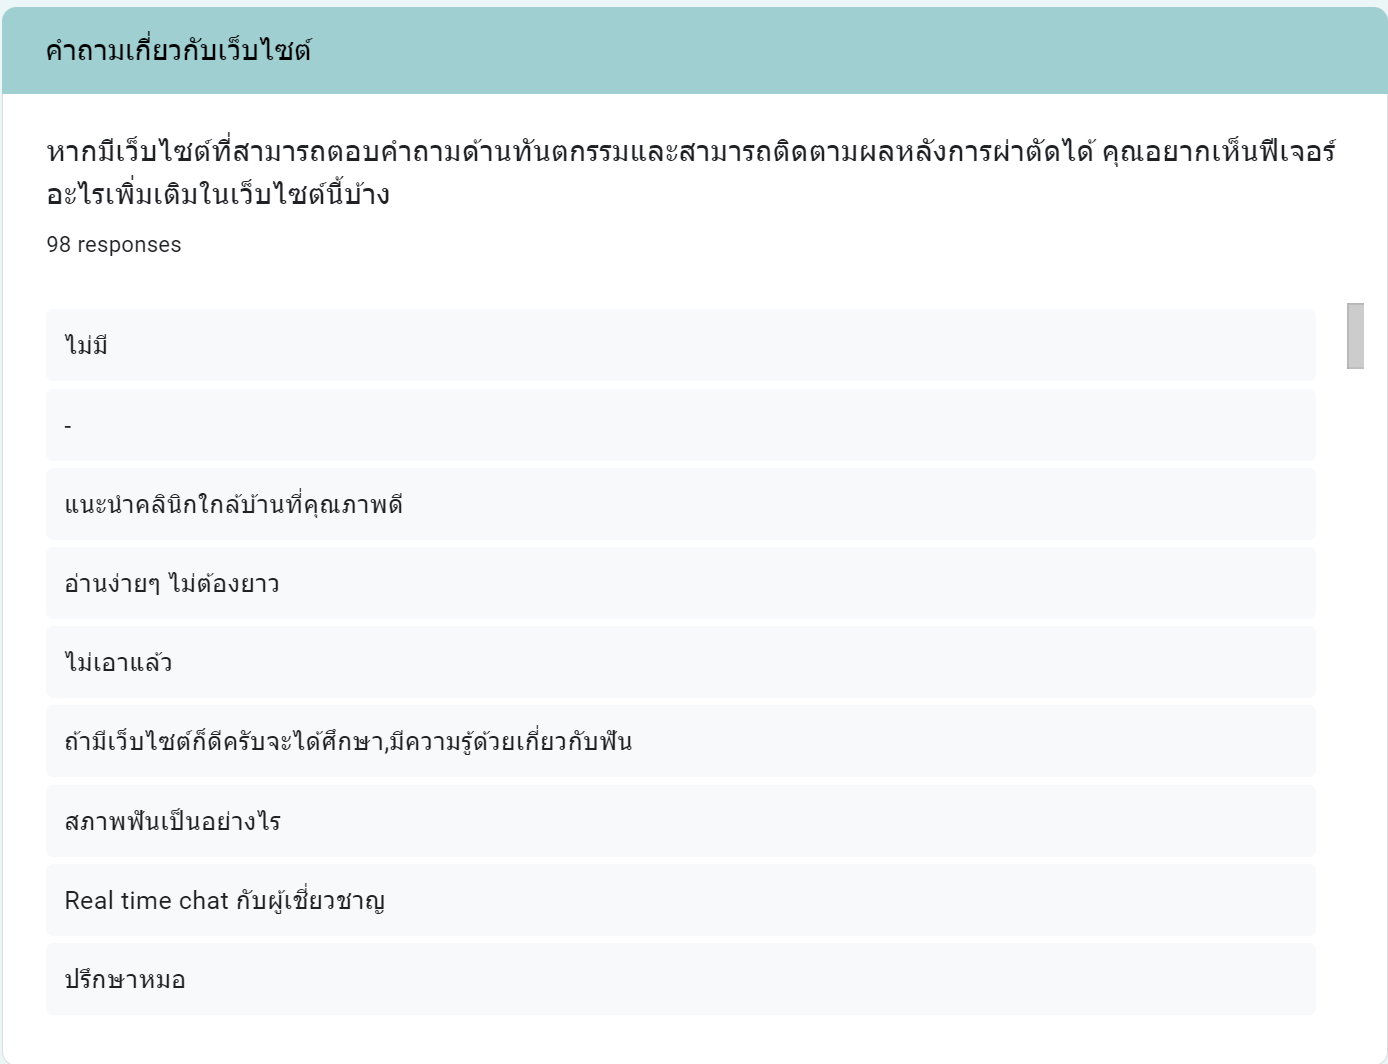
\includegraphics[width=.6\textwidth]{Image/Result_6.png}}
        \caption{Recommendations for Website Development and Features}\label{fig:Result_6}
      \end{figure}
      \FloatBarrier{}
      \qquad The survey results indicate that out of 169 respondents, 63.3 percentage have experienced oral surgery, primarily involving procedures like tooth extraction, wisdom tooth removal, periodontal surgery, and dental implant surgery. The prevalent reason reported for surgery was toothache. Frequently asked questions revolved around surgical procedures, post-operative self-care, necessary care instructions, recommendations, and essential guidelines for proper care. \par
    
  \section{Follow-Up Procedure Interview}
    \qquad As the follow-up process stands as a primary feature of our project, it is essential to thoroughly examine every critical element. This interview aims to emphasize the post-surgery follow-up in the context of dental healthcare, understand the importance of comprehensive patient care, and delve into the specifics of the follow-up process. This comprehension allows us to replicate the actual medical staff procedure effectively.  \par
    \qquad This section elucidates our methodology in conducting interviews with the dental clinic's medical staff to gain important insights into the techniques used for post-surgery tracking. \par
    \subsection{Interviewing Dental Clinic Around the University}
      \qquad To gain an insight into and understand the post-surgery follow-up procedure, we initiated interviews at the dental clinic around the university. The interview questions included inquiries about patient symptom monitoring procedures (\textthai{ขั้นตอนการติดตามอาการผู้ป่วย}), typically how many hours post-surgery patient symptoms are usually followed up (\textthai{โดยปกติแล้วจะทำการโทรติดตามอาการคนไข้กี่ชั่วโมงหลังผ่าตัด}), common inquiries asked to patients during symptom follow-ups (\textthai{คำถามที่มักจะถามผู้ป่วยตอนติดตามอาการ}), and the typical questions patients commonly ask during follow-ups (\textthai{คำถามที่ผู้ป่วยมักจะถามกลับมา}). These interviews provided invaluable insights and a deeper understanding of follow-up procedures, enriching our research with firsthand perspectives on patient care during the post-surgical phase within the local dental healthcare landscape. \par

    \subsection{Interviewing and Survey at Faculty of Dentistry at Chulalongkorn University}
      \qquad According to the important requirement for an in-depth understanding of the practicalities involved with the follow-up procedure, we needed to familiarize ourselves with the patient's involvement following surgery. This includes an in-depth investigation of  complexity of questions, symptom assessment, patient interaction during the follow-up phase, and response to particular concerns. Regarding the complexity of these interactions, we think it is important to have discussions and obtain advice from professionals, especially those who have experience with the follow-up procedure, and patient communication. \par
      \qquad In order to capture the view of the expert and  match our project with the actual demands of both medical professionals and patients, we conduct an on-site observation and interviews at the Faculty of Dentistry, Chulalongkorn University. \par
      \qquad Recognizing the necessity for an in-depth understanding of the practicalities involved in the follow-up procedure, we aimed to acquaint ourselves with the patient involvement post-surgery. This includes a thorough investigation of the intricacies of questions, symptom assessment, patient interaction during follow-ups, and addressing specific concerns. Given the complexity of these interactions, we believed it crucial to engage in discussions and seek advice from professionals, experienced in follow-up procedures, and patient communication. To align our project with the actual demands of both medical professionals and patients, we conducted an on-site observation and interviews at the Faculty of Dentistry, Chulalongkorn University. \par
      \begin{figure}[!h]
        \centering
        \fbox{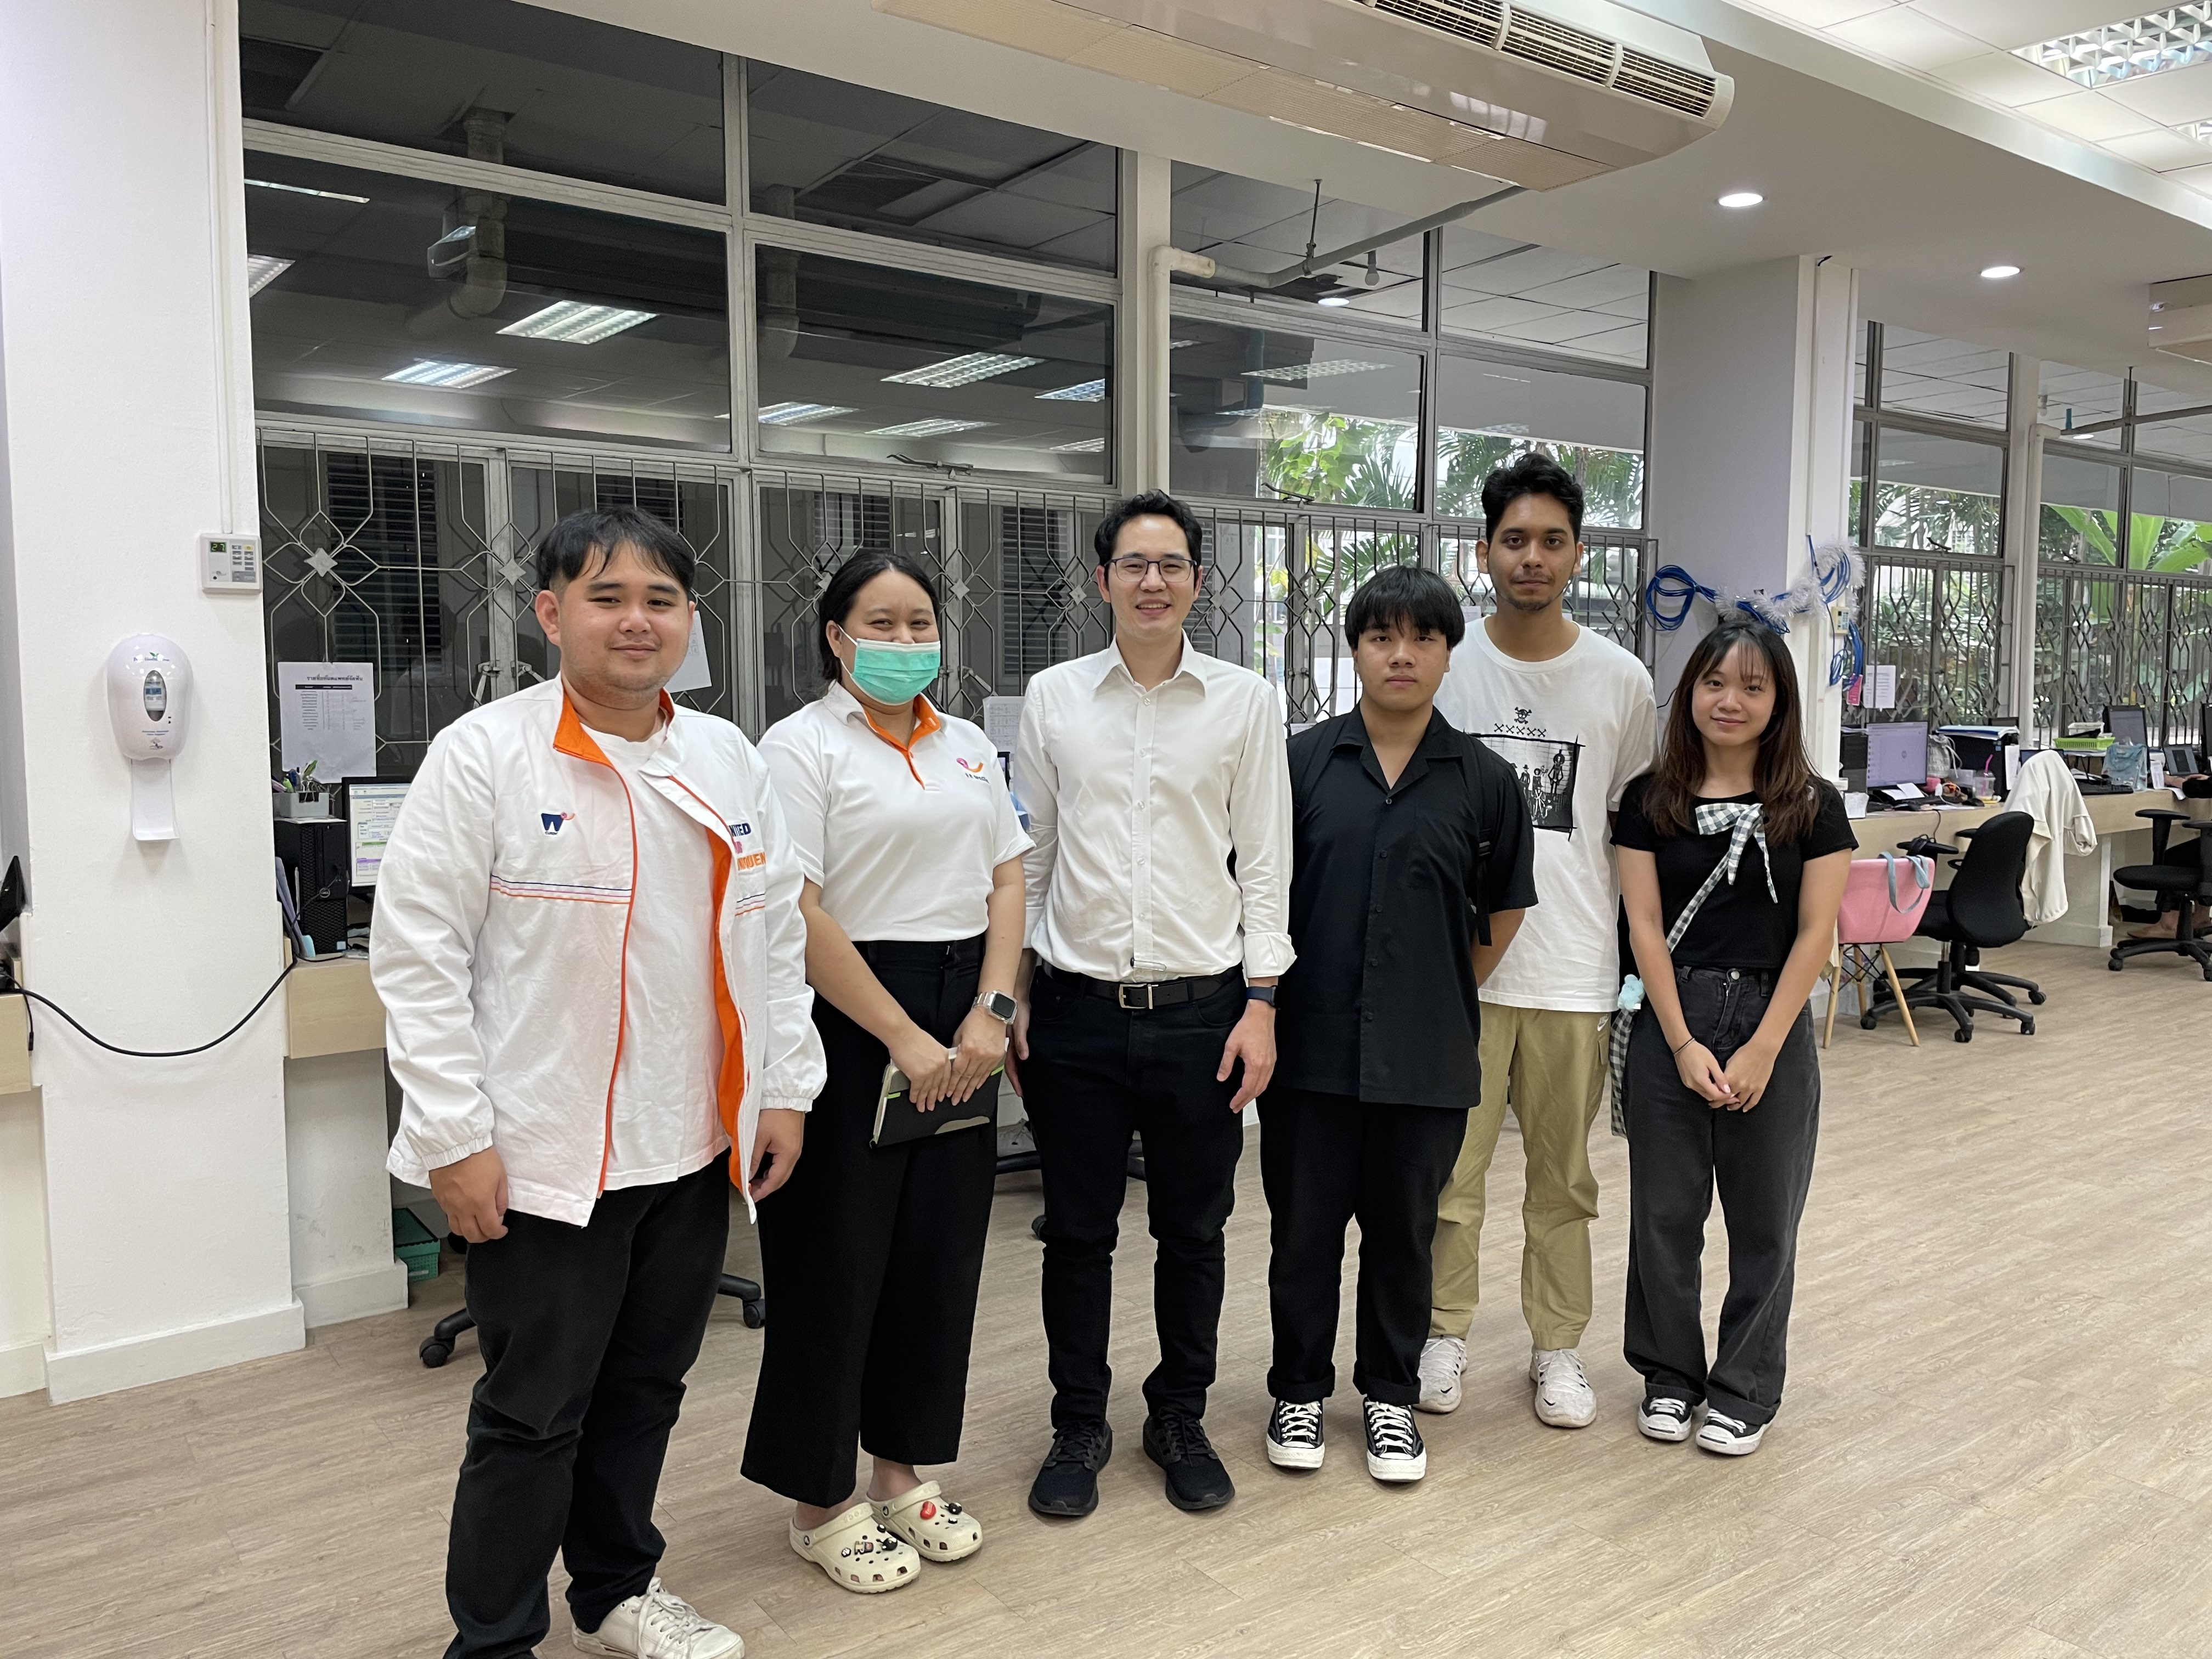
\includegraphics[width=.6\textwidth]{Image/Interview_1.jpg}}
        \caption{Our team and the call-center representative}\label{fig:Interview_1}
        \begin{flushleft}
          \qquad Figure 4.11 depicts our team alongside the call-center representative employed at the OPD Instant Clinic's call center. This department is responsible for answering questions and assisting OPD patients. \par
        \end{flushleft}        
      \end{figure}
      \begin{figure}[!h]
        \centering
        \fbox{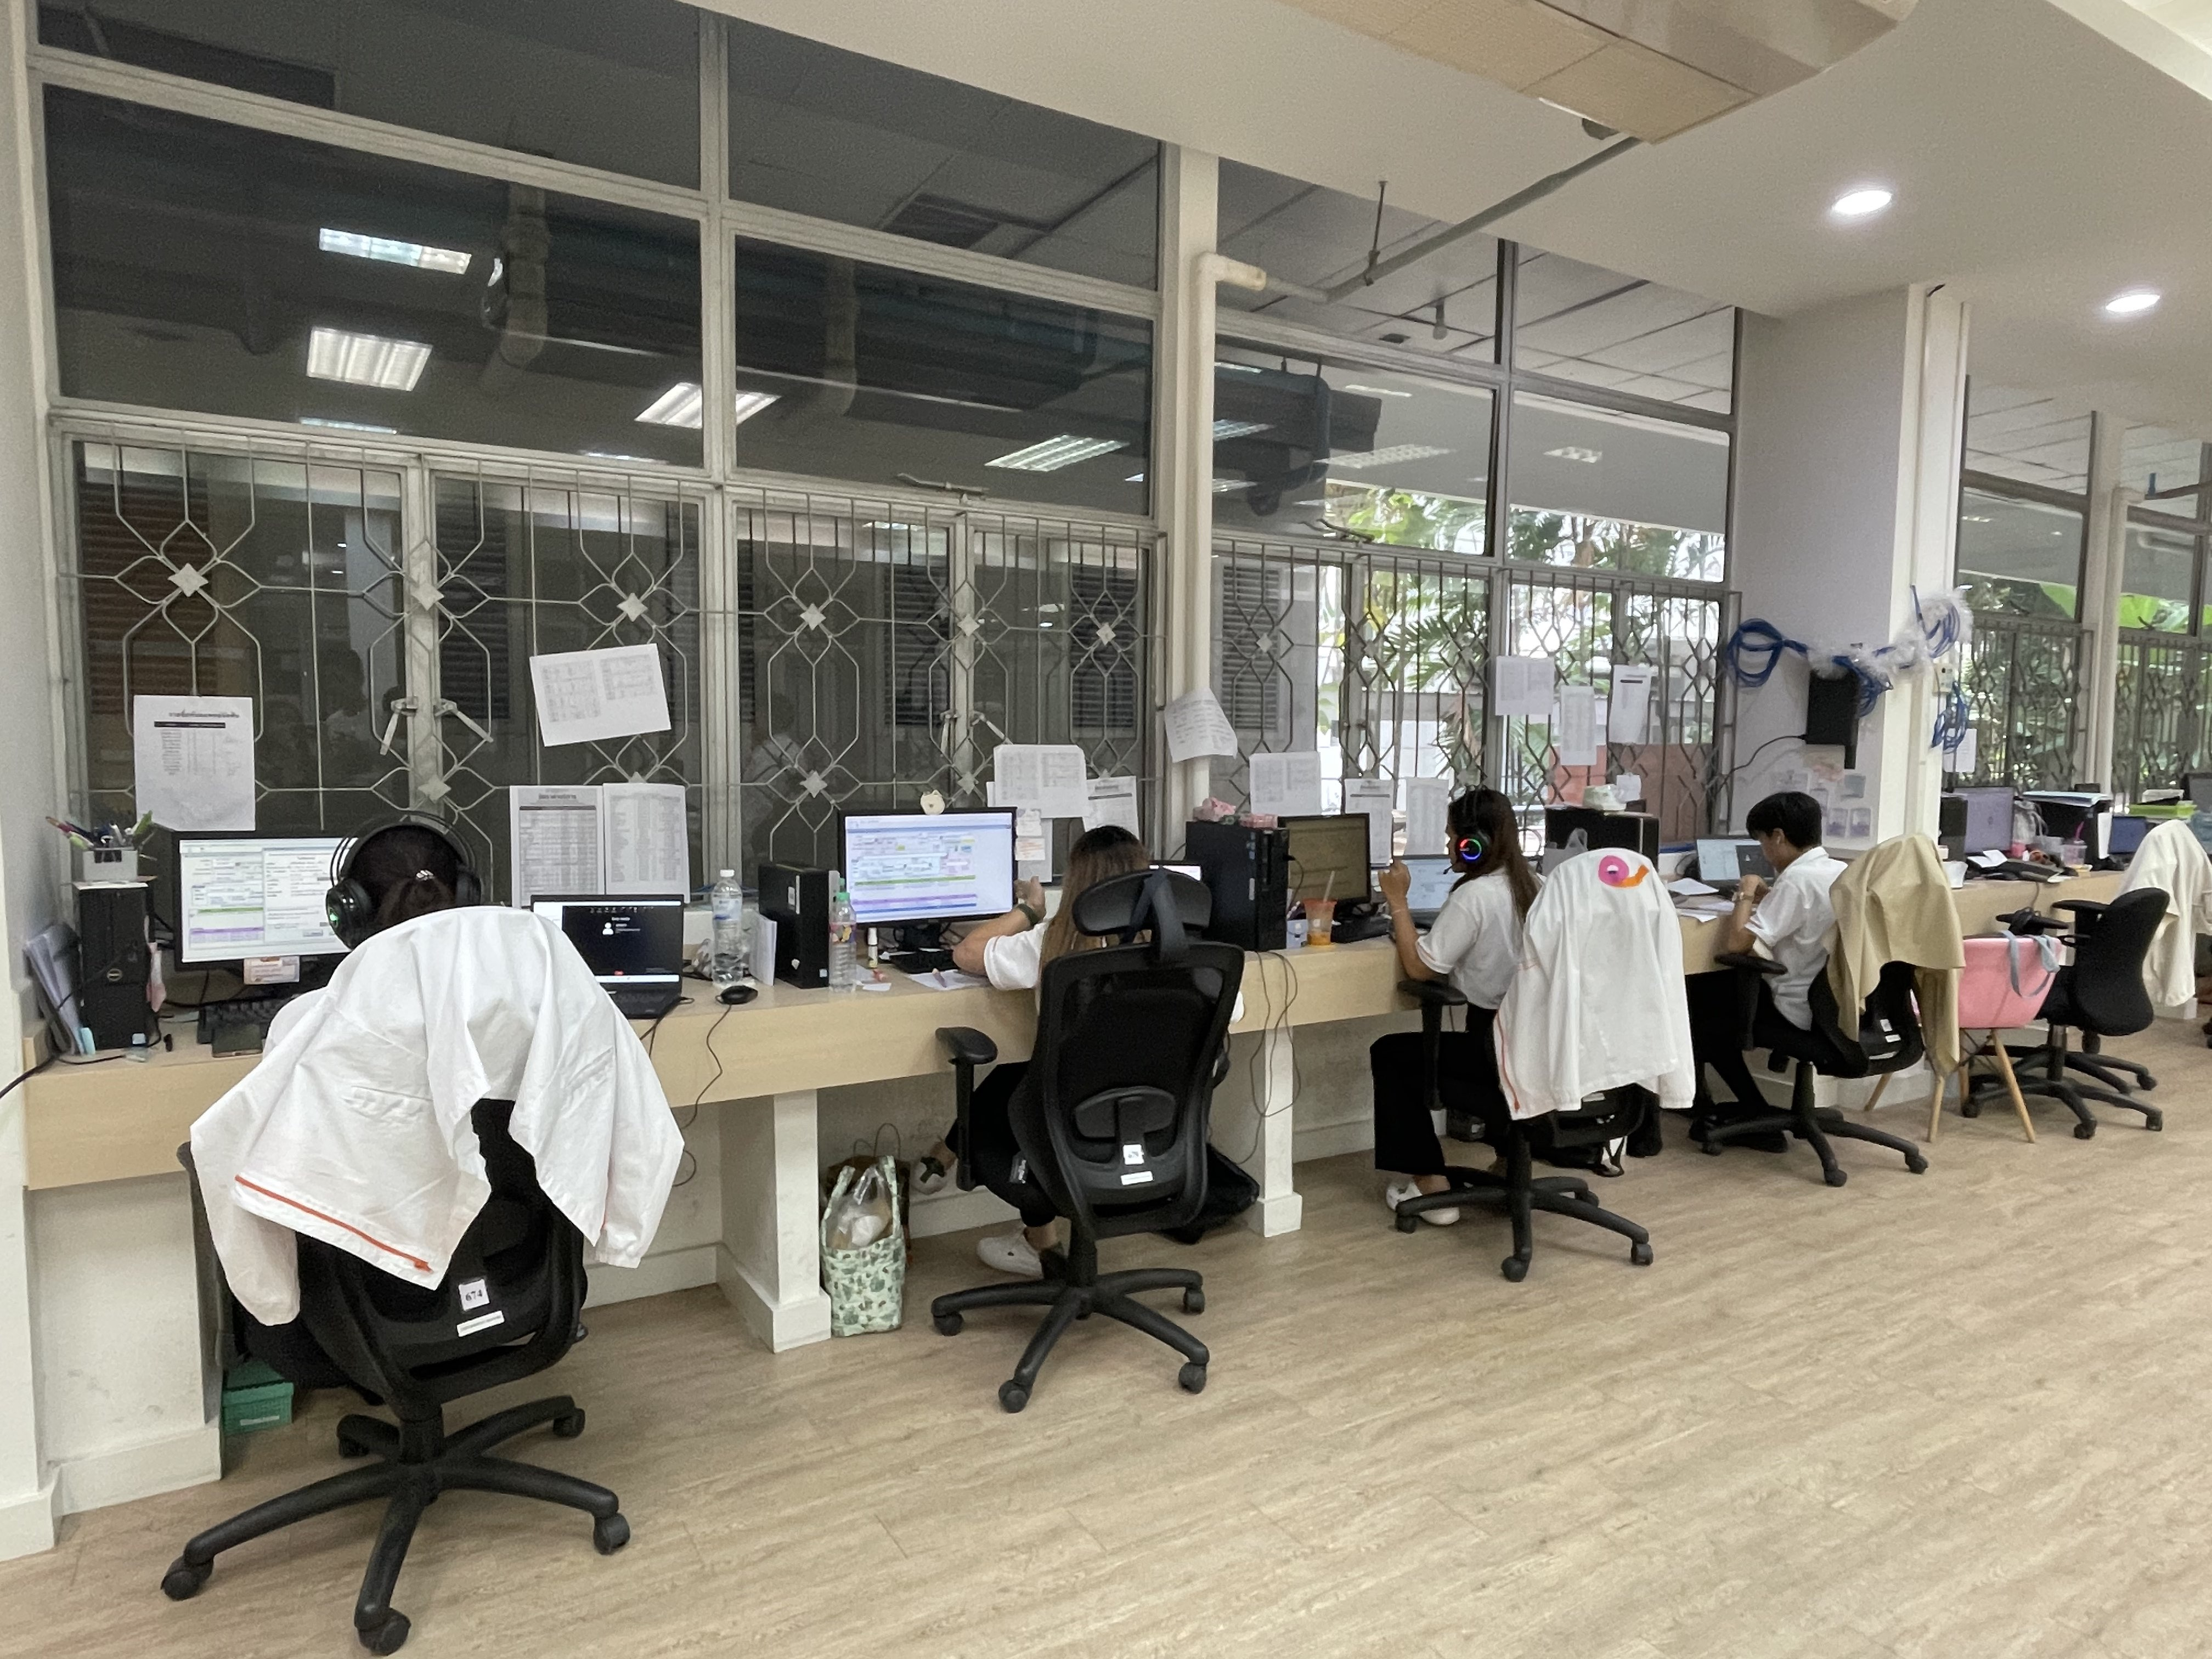
\includegraphics[width=.6\textwidth]{Image/Interview_2.jpg}}
        \caption{Working environment of the OPD Instant Clinic's call center}\label{fig:Interview_2}
        \begin{flushleft}
          \qquad Figure 4.12 shows the operational environment within the OPD Instant Clinic's call center, where staff members engage in follow-up procedures with patients a day after their surgeries. \par
        \end{flushleft}
      \end{figure}
      \begin{figure}
        \centering
        \fbox{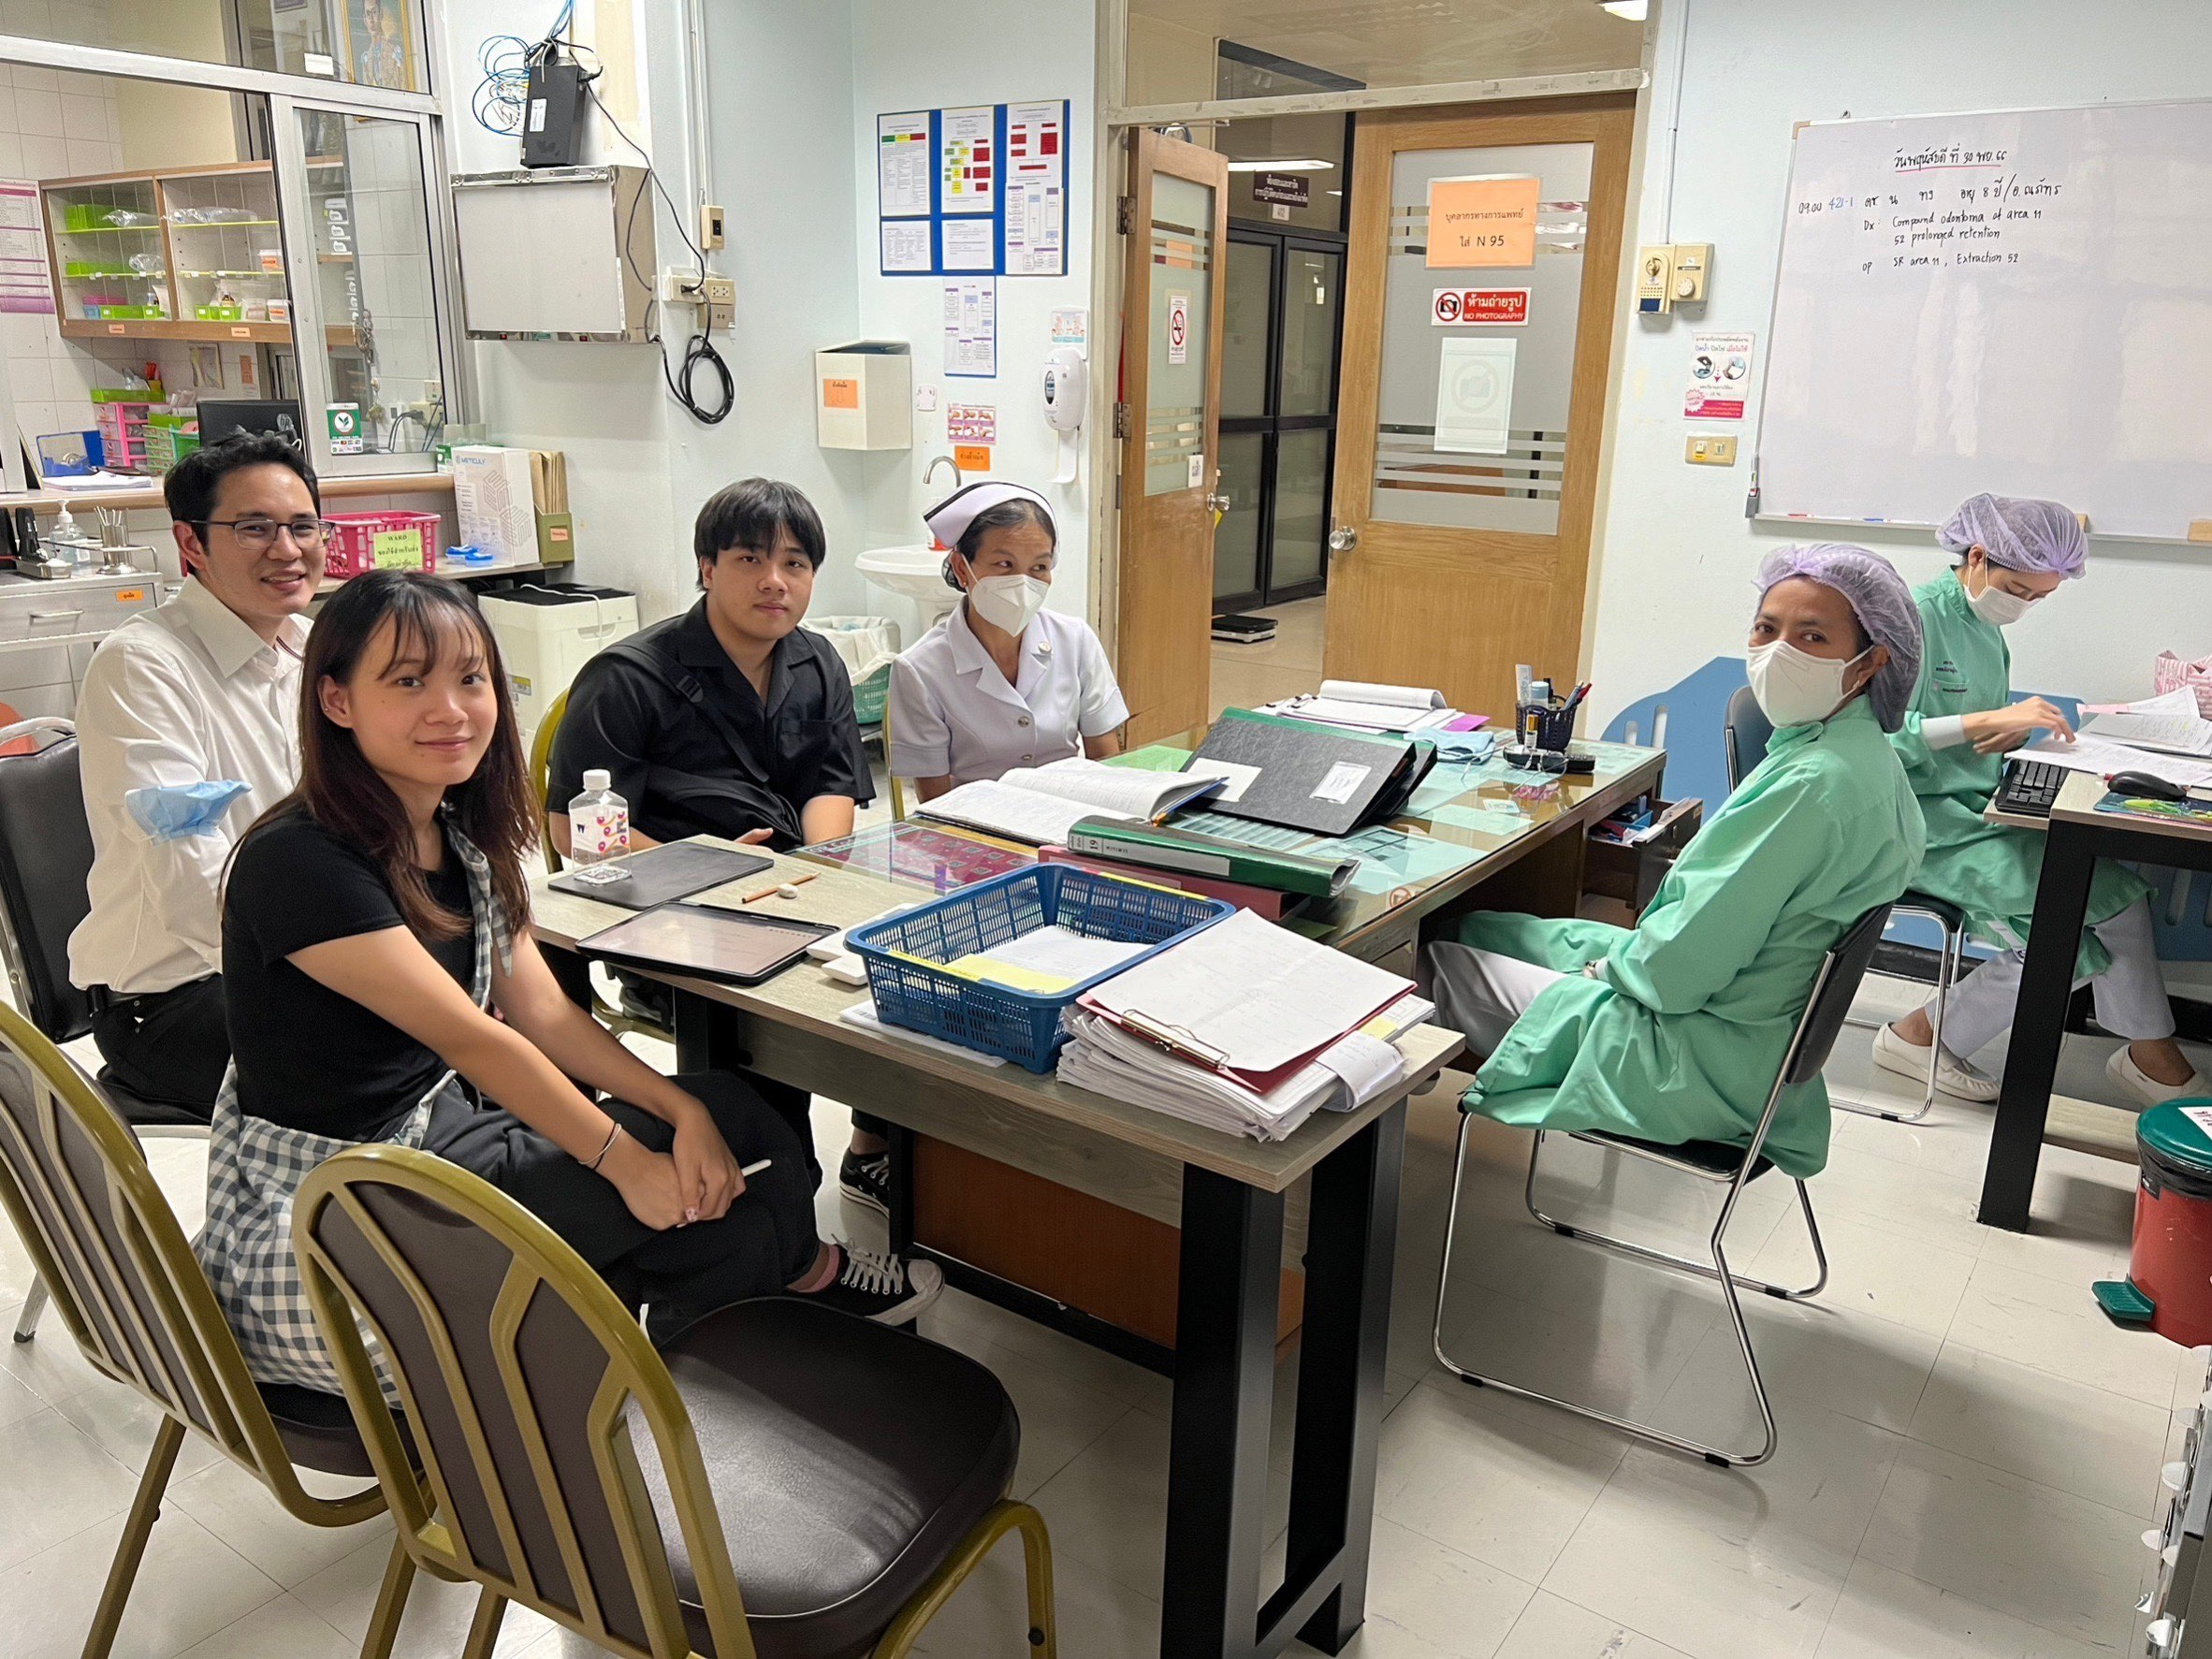
\includegraphics[width=.5\textwidth]{Image/Interview_3.jpg}}
        \caption{Conversation with the nurse who is experienced in the patient follow-up process}\label{fig:Interview_3}
        \begin{flushleft}
          \qquad We engaged in a conversation with an experienced nurse specializing in the patient follow-up process. This follow-up routine typically occurs three days after a patient's discharge, during which the nurse contacts patients and provides necessary advice and support. \par
        \end{flushleft}
      \end{figure}
      \begin{figure}
        \centering
        \fbox{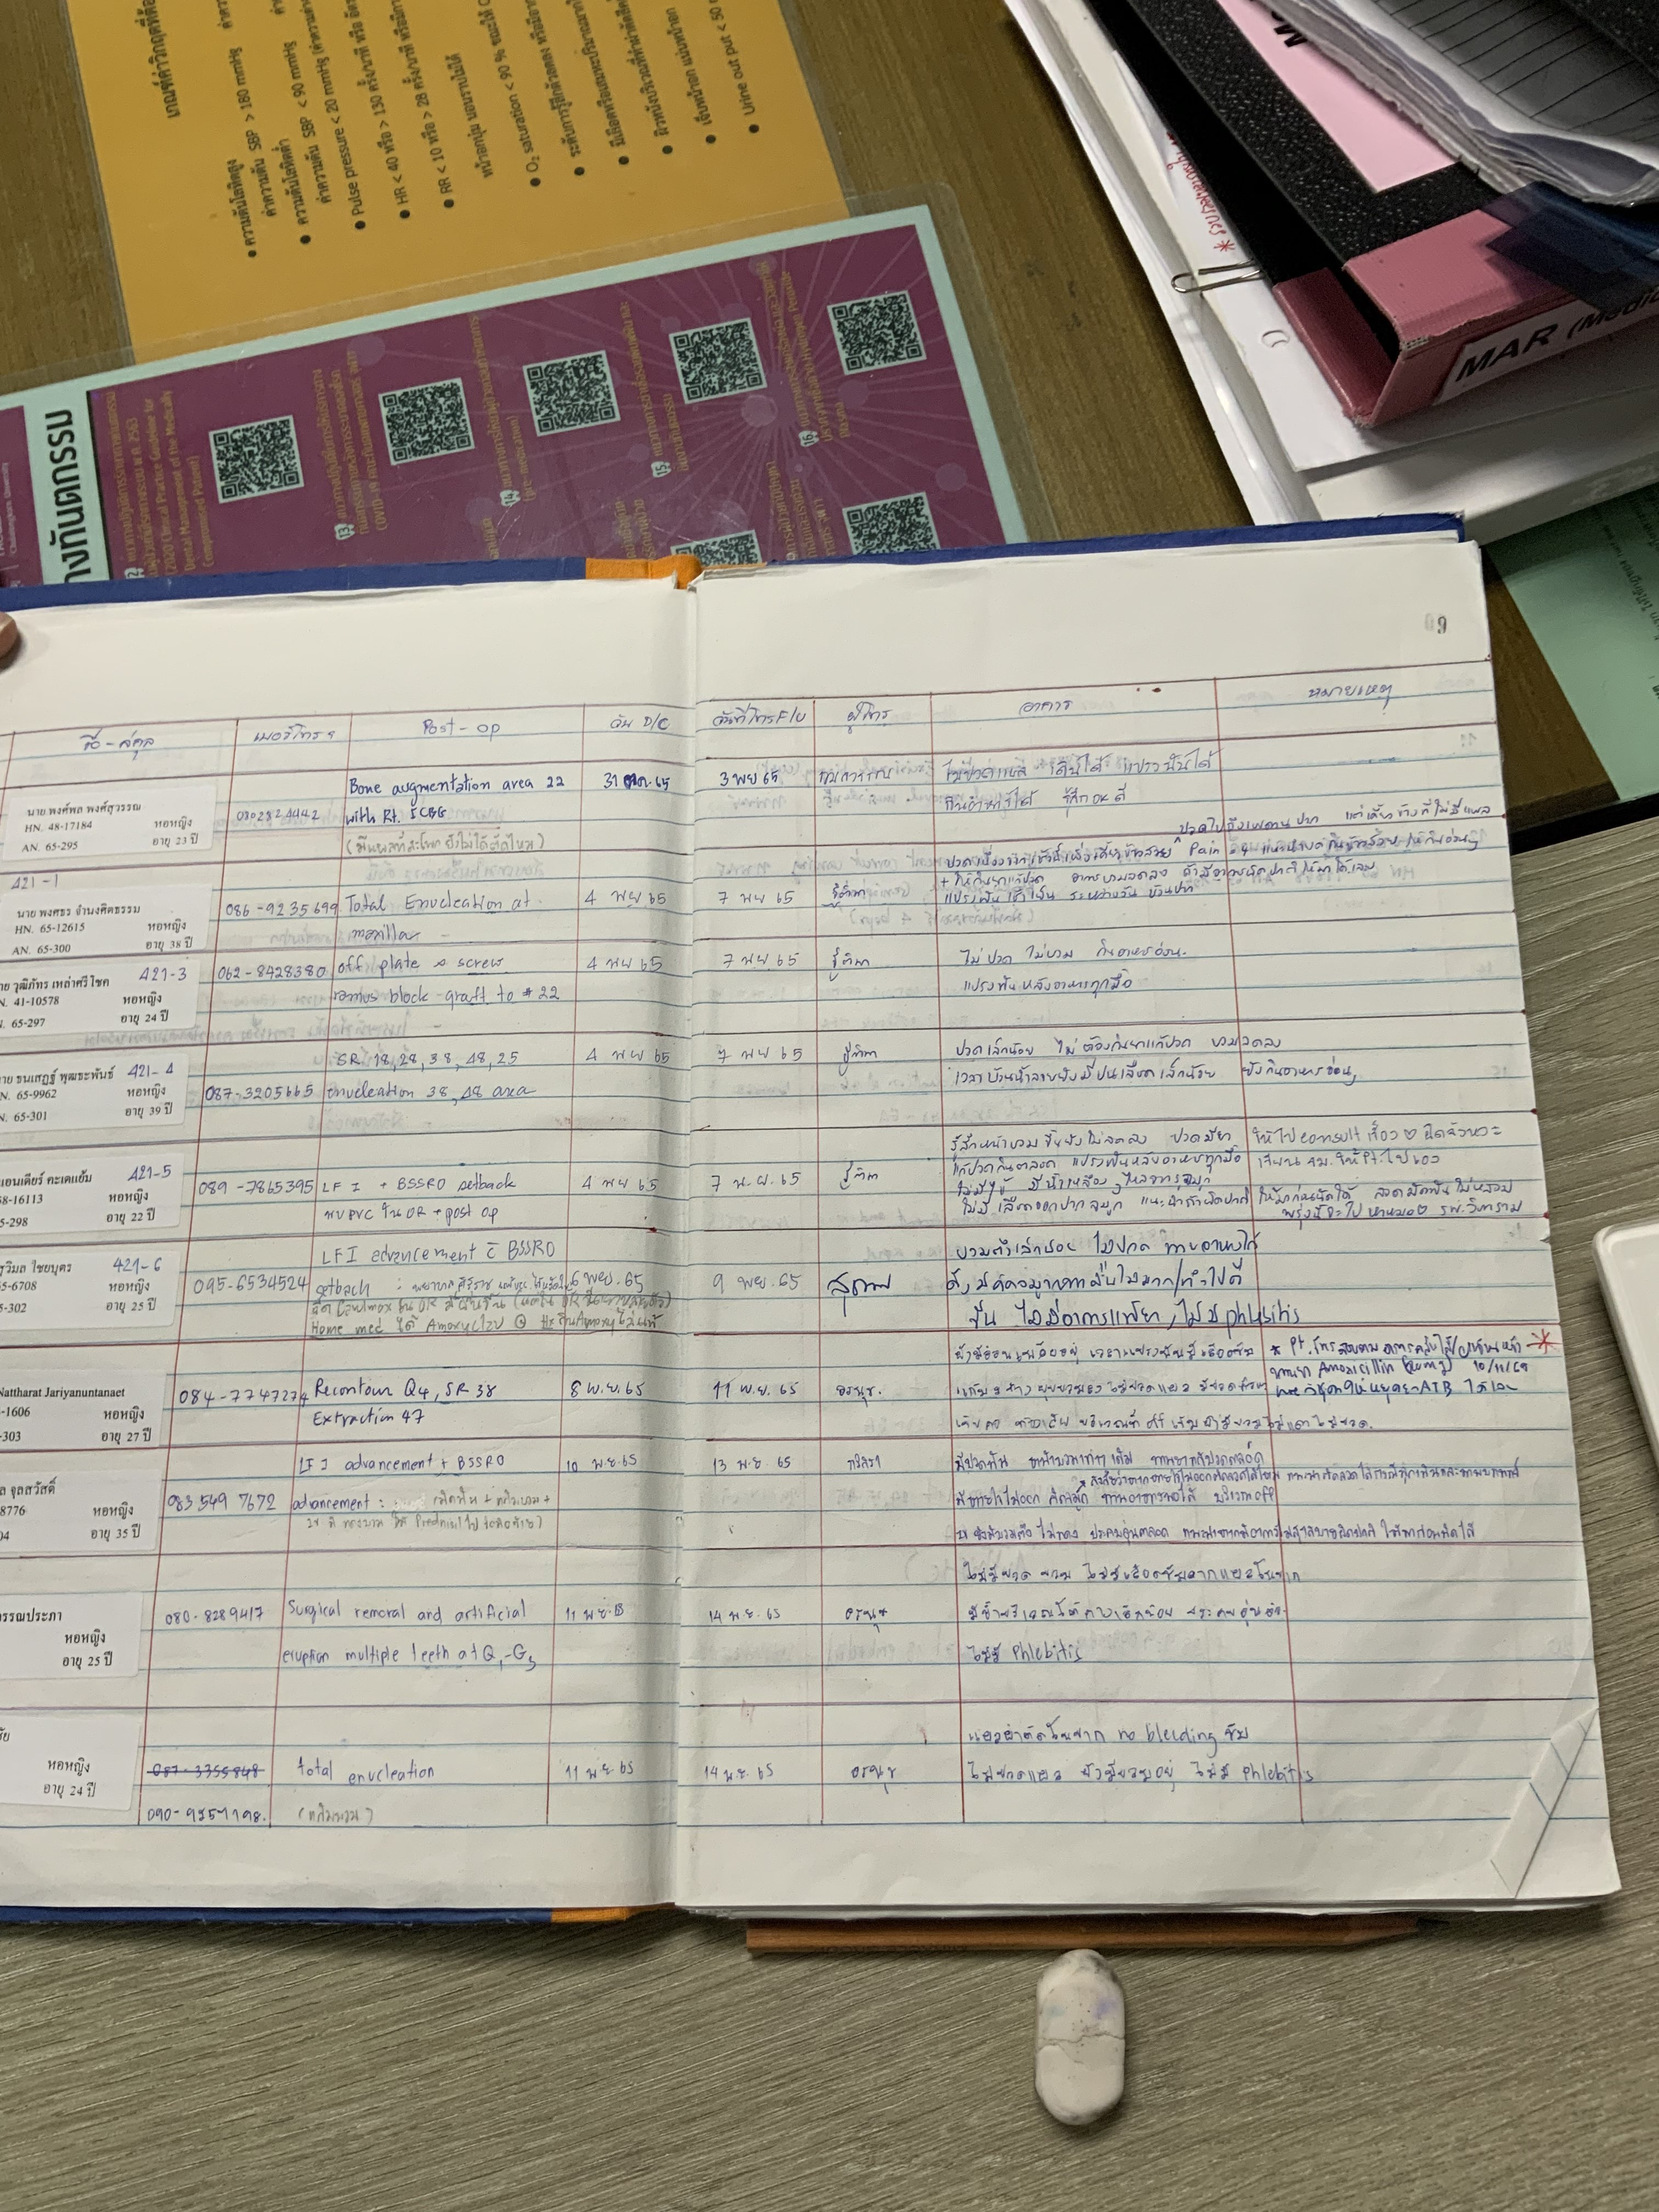
\includegraphics[width=.5\textwidth]{Image/Interview_4.jpg}}
        \caption{Document that the nurse has documented patient information during follow-up sessions}\label{fig:Interview_4}
        \begin{flushleft}
          \qquad Figure 4.14 displays the document used by the nurse to document patient information during follow-up sessions. This documentation includes essential details such as the operation performed, discharge date, follow-up date, contact person, symptoms observed, and any additional notes. This method ensures a comprehensive and precise approach to tracking patient data obtained during follow-up calls. \par
        \end{flushleft}
      \end{figure}
    
  \FloatBarrier{}    
  \section{Frequently Ask Question Dataset}
    \subsection{Prepare Dataset For Training Classification Model}
      \qquad Initially, the dataset of the project had 240 questions, and we wanted to divide the questions into 4 operations according to the scope of this project. However, due to the large amount of content in each operation, we decided to further divide the data of each operation into different 'Question Types' to make the content clearer and easier to use in the subsequent steps of answering questions. \par
      \qquad When attempting to train a classification model to predict the corresponding operation for a given question, we achieved a maximum accuracy of 0.7. However, the model encountered difficulties in accurately predicting certain question types due to insufficient representation of those types in the dataset. To address this issue, we opted to source additional questions from various channels, resulting in a total of 798 questions. Subsequently, we augmented the dataset using techniques including random insertion, random deletion, random swap, back translation, and paraphrased text. This augmentation process resulted in a total of 2,033 questions within the dataset. \par
      \qquad The questions were initially categorized into 5 types \textthai{(ข้อดี, ข้อแนะนำ, ทั่วไป, ปัจจัยเสี่ยง, สาเหตุ)}, which we denoted as Question Type 1 (Q1). However, there was an imbalance in the number of questions across each category, which introduced bias during the training process. Therefore, we attempted to reclassify the question types into 7 new categories (Procedure-related, Post-procedure Care, Symptom-related, Risk-related, Medical-related, Technical-related, and General Health), referred to as Question Type 2 (Q2). This restructuring aimed to achieve a more equitable distribution of questions in our dataset, as illustrated in Figure 4. \par
      \qquad Moreover, during our experimentation with classification models, we noticed instances where certain questions did not clearly align with a specific operation, leading to inaccuracies in the models’ predictions. Therefore, we aggregated such questions into a distinct class labeled "No Class," thereby expanding the total number of operations to 5. \par
      \begin{figure}[!h]
        \centering
        \begin{minipage}{.3\textwidth}
          \centering
          \fbox{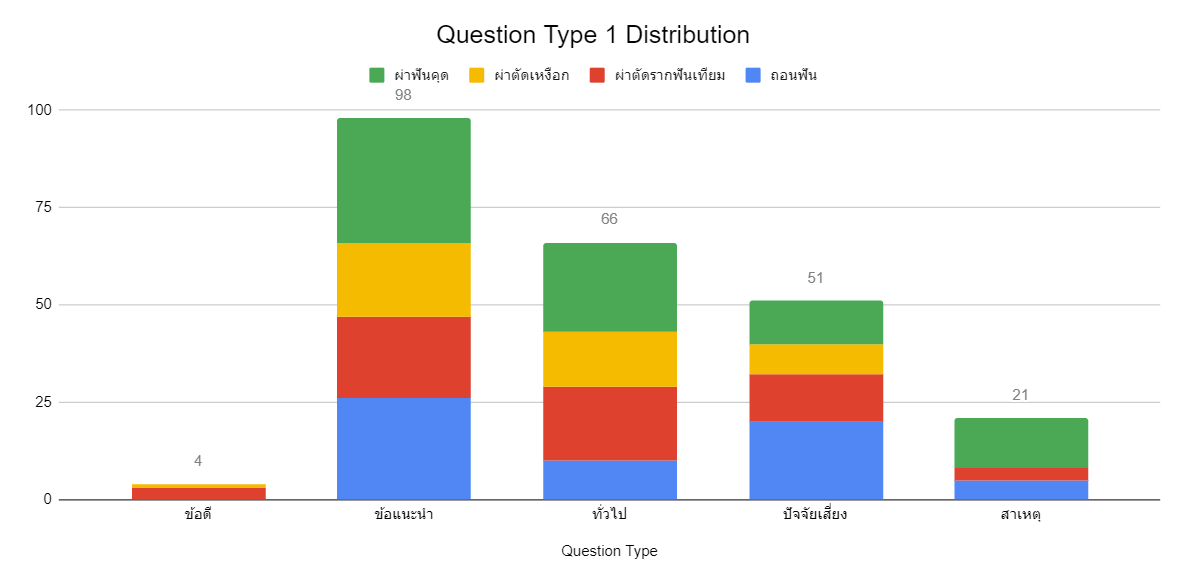
\includegraphics[width=.6\linewidth]{Image/EDAQ1.png}}
        \end{minipage}%
        \begin{minipage}{.3\textwidth}
          \centering
          \fbox{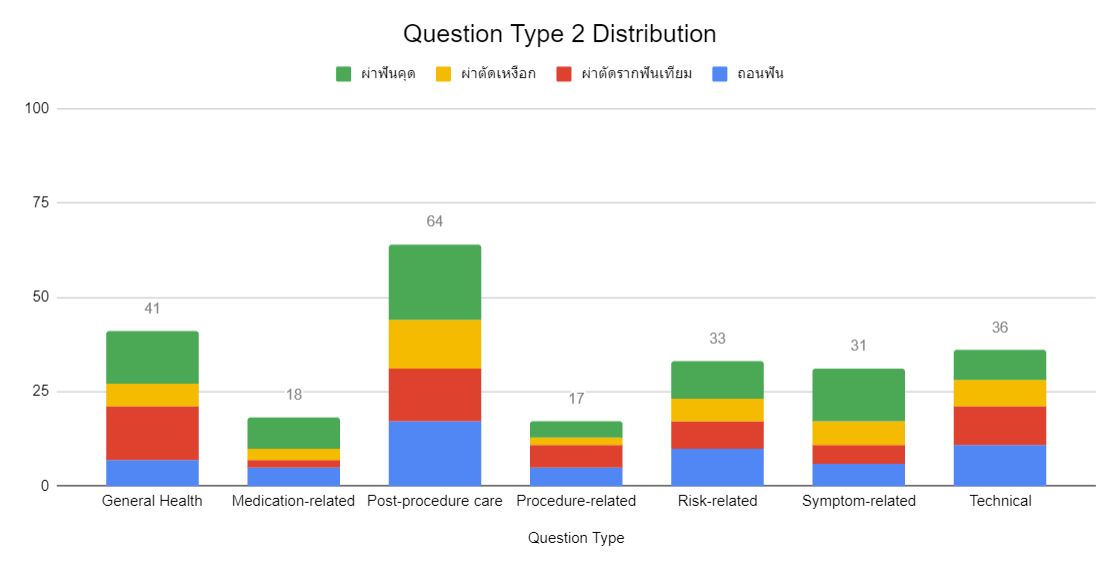
\includegraphics[width=.6\linewidth]{Image/EDAQ2.png}}
        \end{minipage}%
        \caption{Distribution of Question Type}\label{fig:Distribution of Question Type}
      \end{figure}
      
    \subsection{Train and Test Set of Classification Model}
      \qquad In every classification model, training followed a structured approach using three types of datasets, arranged in the following sequence: Normal Dataset, Added Normal Dataset, and Augmented Dataset. The dataset sizes differ to facilitate performance comparison across the models. Each dataset is subdivided into training and testing sets at a ratio of 4:1. \par
      \qquad In tables 4.1 – 4.4, you will observe the inclusion of random state numbers as control variables to regulate the data splitting process within the function. This ensures consistency in test usage across comparisons, a crucial aspect for accurately assessing the model accuracies. \par
      \qquad In the actual dataset, there are a total of 5 operations: \textthai{ถอนฟัน, ผ่าฟันคุด,ผ่าตัดเหงือก, ผ่าตัดรากฟันเทียม} and NC(No Class). However, for training the Operation + Question Type and Operation -> Question Type models, we excluded the NC operation. Consequently, the dataset sizes are reduced to 689 and 1,767 for the Added Normal and Augmented datasets respectively. As for answering NC operation questions, users will be prompted to re-enter their questions while specifying the operation they are inquiring about. Therefore, classifying this operation class is not necessary for the current model objectives. \par
      \begin{table}
        \centering
        \caption{Train and Test Set of Normal and Augmented Dataset Training With Operation+Q1 and Operation+Q2 Classification model}
        \resizebox{\linewidth}{!}{%
        \begin{tabular}{>{\centering\hspace{0pt}}m{0.246\linewidth}>{\centering\hspace{0pt}}m{0.183\linewidth}>{\centering\hspace{0pt}}m{0.235\linewidth}>{\centering\hspace{0pt}}m{0.09\linewidth}>{\centering\hspace{0pt}}m{0.092\linewidth}>{\centering\arraybackslash\hspace{0pt}}m{0.079\linewidth}} 
          \toprule
          \textbf{Training Model} & \textbf{Dataset} & \textbf{Random State} & \textbf{Total} & \textbf{Train} & \textbf{Test}  \\ 
          \toprule
          Operation + Q1          & Normal           & 42                    & 689            & 551            & 138            \\
          Operation + Q2          & Augmented        & 42                    & 1767           & 1413           & 354            \\
          \bottomrule
        \end{tabular}
        }
      \end{table}
      \begin{table}
        \centering
        \caption{Train and Test Set of Normal and Augmented Dataset Training With Operation, Q1, and Q2 Classification Model}
        \resizebox{\linewidth}{!}{%
        \begin{tabular}{>{\centering\hspace{0pt}}m{0.163\linewidth}>{\centering\hspace{0pt}}m{0.081\linewidth}>{\centering\hspace{0pt}}m{0.083\linewidth}>{\centering\hspace{0pt}}m{0.071\linewidth}>{\centering\hspace{0pt}}m{0.325\linewidth}>{\centering\arraybackslash\hspace{0pt}}m{0.212\linewidth}} 
          \toprule
          \textbf{Dataset} & \textbf{Total} & \textbf{Train} & \textbf{Test} & \textbf{Training Model}  & \textbf{Random State}  \\ 
          \toprule
          Normal           & 798            & 638            & 160           & Operation Classification & 42                     \\
                           &                &                &               & Q1 Classification        & 90                     \\
                           &                &                &               & Q2 Classification        & 81                     \\ 
          \toprule
          Augmented        & 2033           & 1626           & 407           & Operation Classification & 42                     \\
                           &                &                &               & Q1 Classification        & 90                     \\
                           &                &                &               & Q2 Classification        & 81                     \\
          \bottomrule
        \end{tabular}
        }
      \end{table}
      \begin{table}
        \centering
        \scriptsize
        \caption{Train and Test Set of Normal and Augmented Dataset Training With Q1-Operation and Q2-Operation Classification model}
        \resizebox{\linewidth}{!}{%
        \begin{tabular}{>{\centering\hspace{0pt}}m{0.194\linewidth}>{\centering\hspace{0pt}}m{0.096\linewidth}>{\centering\hspace{0pt}}m{0.052\linewidth}>{\centering\hspace{0pt}}m{0.117\linewidth}>{\centering\hspace{0pt}}m{0.056\linewidth}>{\centering\hspace{0pt}}m{0.048\linewidth}>{\centering\hspace{0pt}}m{0.056\linewidth}>{\centering\hspace{0pt}}m{0.048\linewidth}>{\centering\hspace{0pt}}m{0.056\linewidth}>{\centering\hspace{0pt}}m{0.048\linewidth}>{\centering\hspace{0pt}}m{0.073\linewidth}>{\centering\arraybackslash\hspace{0pt}}m{0.063\linewidth}} 
          \toprule
          \textbf{Training Model}     & \textbf{Dataset} & \textbf{Total} & \textbf{Random State} & \multicolumn{2}{c}{\textthai{ถอนฟัน}} & \multicolumn{2}{c}{\textthai{ผ่าฟันคุด}} & \multicolumn{2}{c}{\textthai{ผ่าตัดเหงือก}} & \multicolumn{2}{c}{\textthai{ผ่าตัดรากฟันเทียม}}  \\  
          \cmidrule(lr){5-6}\cmidrule(lr){7-8}\cmidrule(lr){9-10}\cmidrule(lr){11-12}
                                      &                  &                &                       & \textbf{Train} & \textbf{Test}                                                  & \textbf{Train} & \textbf{Test}                                                  & \textbf{Train} & \textbf{Test}                                                     & \textbf{Train} & \textbf{Test}                                                                          \\ 
          \toprule
          Q1-Operation Classification & Normal           & 689            & 90                    & 160            & 33                                                             & 148            & 36                                                             & 112            & 27                                                                & 137            & 36                                                                                     \\
          Q2-Operation Classification &                  &                & 81                    & 166            & 27                                                             & 134            & 50                                                             & 117            & 22                                                                & 131            & 42                                                                                     \\
          \toprule
          Q1-Operation Classification & Augmented        & 1767           & 90                    & 373            & 97                                                             & 429            & 96                                                             & 248            & 74                                                                & 357            & 93                                                                                     \\
          Q2-Operation Classification &                  &                & 81                    & 365            & 105                                                            & 429            & 96                                                             & 256            & 66                                                                & 364            & 86                                                                                     \\
          \bottomrule
        \end{tabular}
        }
      \end{table}
      \begin{table}
        \centering
        \scriptsize
        \caption{Train and Test Set of Normal and Augmented Dataset Training With Q1-Operation and NC and Q2-Operation and NC Classification model}
        \resizebox{\linewidth}{!}{%
        \begin{tabular}{>{\centering\hspace{0pt}}m{0.194\linewidth}>{\centering\hspace{0pt}}m{0.096\linewidth}>{\centering\hspace{0pt}}m{0.052\linewidth}>{\centering\hspace{0pt}}m{0.117\linewidth}>{\centering\hspace{0pt}}m{0.056\linewidth}>{\centering\hspace{0pt}}m{0.048\linewidth}>{\centering\hspace{0pt}}m{0.056\linewidth}>{\centering\hspace{0pt}}m{0.048\linewidth}>{\centering\hspace{0pt}}m{0.056\linewidth}>{\centering\hspace{0pt}}m{0.048\linewidth}>{\centering\hspace{0pt}}m{0.073\linewidth}>{\centering\arraybackslash\hspace{0pt}}m{0.063\linewidth}} 
          \toprule
          \textbf{Training Model}        & \textbf{Dataset} & \textbf{Total} & \textbf{Random State} & \multicolumn{2}{c}{\textthai{ถอนฟัน}} & \multicolumn{2}{c}{\textthai{ผ่าฟันคุด}} & \multicolumn{2}{c}{\textthai{ผ่าตัดเหงือก}} & \multicolumn{2}{c}{\textthai{ผ่าตัดรากฟันเทียม}}  \\  
          \cmidrule(lr){5-6}\cmidrule(lr){7-8}\cmidrule(lr){9-10}\cmidrule(lr){11-12}
                                         &                  &                &                       & \textbf{Train} & \textbf{Test}        & \textbf{Train} & \textbf{Test}        & \textbf{Train} & \textbf{Test}            & \textbf{Train} & \textbf{Test}                 \\ 
          \toprule
          Q1-Operation NC Classification & Normal           & 1125           & 90                    & 241            & 61                   & 229            & 64                   & 193            & 55                       & 218            & 64                            \\
          Q2-Operation NC Classification &                  &                & 81                    & 256            & 46                   & 224            & 69                   & 207            & 41                       & 221            & 61                            \\
          \toprule
          Q1-Operation NC Classification & Augmented        & 2831           & 90                    & 592            & 144                  & 648            & 143                  & 467            & 121                      & 576            & 140                           \\
          Q2-Operation NC Classification &                  &                & 81                    & 577            & 159                  & 641            & 150                  & 468            & 120                      & 576            & 140                           \\
          \bottomrule
        \end{tabular}
        }
      \end{table}
  \section{Question Answering Feature Flow}
    \begin{figure}
      \centering
      \fbox{\includegraphics[width=.5\textwidth]{Image/FAQ-flow.png}}
      \caption{FAQ Flow}\label{fig:FAQ Flow}
      \begin{flushleft}
        \qquad Initially, the design question answering feature flow involves taking questions received from users and using them to find labels with the classification model. Then, the labels are matched with contexts that have the same labels. Then use both the question and the context to find the answer to the question using the question-answering pretrained model (DeBERTa). \par
      \end{flushleft}
    \end{figure}
  \section{Classification Model Experiment}
    \qquad In our experimentation with training models for classifying question types, we chose to explore various machine learning approaches. Specifically, we employed the Python modules sklearn.naivebayes and sklearn.ensemble to utilize a range of algorithms including BernoulliNB, MultinomialNB, GaussianNB, ComplementNB, CategoricalNB, and RandomForestClassifier. Additionally, we employed a technique known as grid search, which involves systematically searching for the optimal hyperparameters by specifying potential values for each machine learning algorithm. This grid search approach enables efficient identification of the best hyperparameters, thereby saving time in tuning each model. The results from all models were derived from testing against two types of test sets: the normal test set and the augmented test set.  The main difference between these two test sets lies in the presence of typing errors, whereas the augmented test set includes samples with simulated typing errors added using the text augmentation technique outlined in section 2.3.7, applied to the normal dataset. \par
    \qquad Through our experimentation, we explored three main types of classification methodologies: Simple Classification, Parallel Classification, and Sequential Classification. In Parallel Classification, the label prediction for a question occurs concurrently using both the operation model and the question type model. Sequential Classification involves predicting the label for a question first using the operation model and subsequently using the question type model trained with data specific to each operation. Lastly, Simple Classification pairs each operation with its corresponding question type and utilizes a single model to predict the label for the matched pair. \par
    \subsection{Operation Classification }
      \qquad In our quest to determine the optimal model for predicting the operation of each question, we opted to leverage machine learning techniques. Upon analyzing the dataset, we observed that many questions already contain distinct keywords that hint at the associated operations. Consequently, we embarked on further experimentation by incorporating a Keyword Search technique into our methodology. \par
      \subsubsection{Machine Learning Model}
        \begin{table}
          \scriptsize
          \centering
          \caption{Operation Classification with Added Normal and Augmented Experiment Result (Machine Learning)}
          \resizebox{\linewidth}{!}{%
          \begin{tabular}{>{\centering\hspace{0pt}}m{0.081\linewidth}>{\centering\hspace{0pt}}m{0.071\linewidth}>{\centering\hspace{0pt}}m{0.06\linewidth}>{\centering\hspace{0pt}}m{0.069\linewidth}>{\centering\hspace{0pt}}m{0.06\linewidth}>{\centering\hspace{0pt}}m{0.069\linewidth}>{\centering\hspace{0pt}}m{0.06\linewidth}>{\centering\hspace{0pt}}m{0.069\linewidth}>{\centering\hspace{0pt}}m{0.06\linewidth}>{\centering\hspace{0pt}}m{0.069\linewidth}>{\centering\hspace{0pt}}m{0.062\linewidth}>{\centering\hspace{0pt}}m{0.069\linewidth}>{\centering\hspace{0pt}}m{0.06\linewidth}>{\centering\arraybackslash\hspace{0pt}}m{0.069\linewidth}} 
            \toprule
            \textbf{Dataset} & \textbf{Measure} & \multicolumn{2}{c}{\textbf{Random Forest}} & \multicolumn{2}{c}{\textbf{Multinomial NB}} & \multicolumn{2}{c}{\textbf{Gaussian NB}} & \multicolumn{2}{c}{\textbf{Bernoulli NB}} & \multicolumn{2}{>{\centering\hspace{0pt}}m{0.131\linewidth}}{\textbf{Complement NB}} & \multicolumn{2}{>{\centering\arraybackslash\hspace{0pt}}m{0.129\linewidth}}{\textbf{Categorical NB}}  \\ 
            \cmidrule(lr){3-4}\cmidrule(lr){5-6}\cmidrule(lr){7-8}\cmidrule(lr){9-10}\cmidrule(lr){11-12}\cmidrule(lr){13-14}
                             &                  & Normal & Augment                                                                     & Normal & Augment                                                                      & Normal & Augment                                                                   & Normal & Augment                                                                    & Normal & Augment                                                                     & Normal & Augment                                                                                      \\ 
            \toprule
            Normal           & Accuracy         & 0.844  & 0.889                                                                       & 0.863  & 0.887                                                                        & 0.906  & 0.889                                                                     & 0.888  & 0.892                                                                      & 0.844  & 0.889                                                                       & 0.819  & 0.887                                                                                        \\
                             & F1-Score         & 0.844  & 0.890                                                                       & 0.861  & 0.886                                                                        & 0.902  & 0.887                                                                     & 0.881  & 0.893                                                                      & 0.844  & 0.890                                                                       & 0.814  & 0.887                                                                                        \\ 
            \toprule
            Augmented        & Accuracy         & 0.975  & 0.941                                                                       & 0.981  & 0.921                                                                        & 0.950  & 0.899                                                                     & 0.981  & 0.931                                                                      & 0.963  & 0.894                                                                       & 0.981  & 0.934                                                                                        \\
                             & F1-Score         & 0.975  & 0.941                                                                       & 0.981  & 0.921                                                                        & 0.950  & 0.900                                                                     & 0.981  & 0.931                                                                      & 0.963  & 0.891                                                                       & 0.981  & 0.934                                                                                        \\
            \bottomrule
          \end{tabular}
          }
        \end{table}
        \qquad Table 4.5 illustrates that for the added normal dataset, the Gaussian Naïve Bayes model achieved the highest accuracy of 0.906 on the normal test set. Additionally, for the augmented dataset, the Categorical Naïve Bayes model resulted in the highest accuracy of 0.981on the normal test set. \par
      \subsubsection{Keyword Search}
        \begin{table}
          \centering
          \caption{Operation Classification with Added Normal and Augmented Experiment Result (Keyword Search)}
          \resizebox{\linewidth}{!}{%
          \begin{tabular}{>{\centering\hspace{0pt}}m{0.158\linewidth}>{\centering\hspace{0pt}}m{0.127\linewidth}>{\centering\hspace{0pt}}m{0.238\linewidth}>{\centering\hspace{0pt}}m{0.14\linewidth}>{\centering\arraybackslash\hspace{0pt}}m{0.262\linewidth}} 
            \toprule
            \textbf{Measure} & \multicolumn{2}{>{\centering\hspace{0pt}}m{0.365\linewidth}}{\textbf{Keyword Search}} & \multicolumn{2}{>{\centering\arraybackslash\hspace{0pt}}m{0.402\linewidth}}{\textbf{Keyword Search Regex}}  \\ 
            \cmidrule(lr){2-3}\cmidrule(lr){4-5}
                             & Normal & Augment                                                                      & Normal & Augment                                                                                            \\ 
            \toprule
            Accuracy         & 1.00   & 0.7899655681                                                                 & 1.00   & 0.9901623217                                                                                       \\
            F1-Score         & 1.00   & 0.8147365591                                                                 & 1.00   & 0.9902791281                                                                                       \\
            \bottomrule
          \end{tabular}
          }
        \end{table}
        \qquad For Keyword Search, we evaluated the algorithm’s accuracy using the entire dataset, comprising 798 samples for the Normal Data and 2,033 for the Augmented Data. Among the different search methods, Keyword Search2, which employs regular expressions to search for words, outperformed other conventional search techniques in the augmented dataset. This superiority is attributed to its capability to accommodate input questions with errors, leading to significantly improved performance. \par
    \subsection{Simple  Classification}
      \subsubsection{Operation + Q1 Classification}
        \begin{table}
          \scriptsize
          \centering
          \caption{Simple Classification Operation + Q1 Result}
          \resizebox{\linewidth}{!}{%
          \begin{tabular}{>{\centering\hspace{0pt}}m{0.081\linewidth}>{\centering\hspace{0pt}}m{0.071\linewidth}>{\centering\hspace{0pt}}m{0.06\linewidth}>{\centering\hspace{0pt}}m{0.069\linewidth}>{\centering\hspace{0pt}}m{0.06\linewidth}>{\centering\hspace{0pt}}m{0.069\linewidth}>{\centering\hspace{0pt}}m{0.06\linewidth}>{\centering\hspace{0pt}}m{0.069\linewidth}>{\centering\hspace{0pt}}m{0.06\linewidth}>{\centering\hspace{0pt}}m{0.069\linewidth}>{\centering\hspace{0pt}}m{0.062\linewidth}>{\centering\hspace{0pt}}m{0.069\linewidth}>{\centering\hspace{0pt}}m{0.06\linewidth}>{\centering\arraybackslash\hspace{0pt}}m{0.069\linewidth}} 
            \toprule
            \textbf{Dataset} & \textbf{Measure} & \multicolumn{2}{c}{\textbf{Random Forest}} & \multicolumn{2}{c}{\textbf{Multinomial NB}} & \multicolumn{2}{c}{\textbf{Gaussian NB}} & \multicolumn{2}{c}{\textbf{Bernoulli NB}} & \multicolumn{2}{>{\centering\hspace{0pt}}m{0.131\linewidth}}{\textbf{Complement NB}} & \multicolumn{2}{>{\centering\arraybackslash\hspace{0pt}}m{0.129\linewidth}}{\textbf{Categorical NB}}  \\ 
            \cmidrule(lr){3-4}\cmidrule(lr){5-6}\cmidrule(lr){7-8}\cmidrule(lr){9-10}\cmidrule(lr){11-12}\cmidrule(lr){13-14}
                             &                  & Normal & Augment                                                                     & Normal & Augment                                                                      & Normal & Augment                                                                   & Normal & Augment                                                                    & Normal & Augment                                                                     & Normal & Augment                                                                                      \\ 
            \toprule
            Normal           & Accuracy         & 0.572  & 0.766                                                                       & 0.623  & 0.828                                                                        & 0.551  & 0.777                                                                     & 0.638  & 0.774                                                                      & 0.558  & 0.661                                                                       & 0.681  & 0.842                                                                                        \\
                             & F1-Score         & 0.537  & 0.755                                                                       & 0.621  & 0.820                                                                        & 0.557  & 0.780                                                                     & 0.620  & 0.755                                                                      & 0.527  & 0.637                                                                       & 0.683  & 0.835                                                                                        \\ 
            \toprule
            Augmented        & Accuracy         & 0.920  & 0.842                                                                       & 0.877  & 0.825                                                                        & 0.920  & 0.734                                                                     & 0.913  & 0.836                                                                      & 0.754  & 0.684                                                                       & 0.906  & 0.845                                                                                        \\
                             & F1-Score         & 0.921  & 0.841                                                                       & 0.872  & 0.816                                                                        & 0.921  & 0.733                                                                     & 0.913  & 0.846                                                                      & 0.746  & 0.662                                                                       & 0.902  & 0.841                                                                                        \\
            \bottomrule
          \end{tabular}
          }
        \end{table}
        \qquad In the added normal dataset, the Categorical Naïve Bayes model achieved the highest accuracy of 0.681 on the normal test set. For the augmented dataset, both the Random Forest and Gaussian Naïve Bayes models attained the highest accuracy of 0.920 on the normal test set. Consequently, when evaluating accuracy from testing with augmented test data, it was determined that the Random Forest model exhibited the highest accuracy, as shown in Table 4.7. \par
      \subsubsection{Operation + Q2 Classification}
        \begin{table}
          \scriptsize
          \centering
          \caption{Simple Classification Operation + Q2 Result}
          \resizebox{\linewidth}{!}{%
          \begin{tabular}{>{\centering\hspace{0pt}}m{0.081\linewidth}>{\centering\hspace{0pt}}m{0.071\linewidth}>{\centering\hspace{0pt}}m{0.06\linewidth}>{\centering\hspace{0pt}}m{0.069\linewidth}>{\centering\hspace{0pt}}m{0.06\linewidth}>{\centering\hspace{0pt}}m{0.069\linewidth}>{\centering\hspace{0pt}}m{0.06\linewidth}>{\centering\hspace{0pt}}m{0.069\linewidth}>{\centering\hspace{0pt}}m{0.06\linewidth}>{\centering\hspace{0pt}}m{0.069\linewidth}>{\centering\hspace{0pt}}m{0.062\linewidth}>{\centering\hspace{0pt}}m{0.069\linewidth}>{\centering\hspace{0pt}}m{0.06\linewidth}>{\centering\arraybackslash\hspace{0pt}}m{0.069\linewidth}} 
            \toprule
            \textbf{Dataset} & \textbf{Measure} & \multicolumn{2}{c}{\textbf{Random Forest}} & \multicolumn{2}{c}{\textbf{Multinomial NB}} & \multicolumn{2}{c}{\textbf{Gaussian NB}} & \multicolumn{2}{c}{\textbf{Bernoulli NB}} & \multicolumn{2}{>{\centering\hspace{0pt}}m{0.131\linewidth}}{\textbf{Complement NB}} & \multicolumn{2}{>{\centering\arraybackslash\hspace{0pt}}m{0.129\linewidth}}{\textbf{Categorical NB}}  \\ 
            \cmidrule(lr){3-4}\cmidrule(lr){5-6}\cmidrule(lr){7-8}\cmidrule(lr){9-10}\cmidrule(lr){11-12}\cmidrule(lr){13-14}
                             &                  & Normal & Augment                                                                     & Normal & Augment                                                                      & Normal & Augment                                                                   & Normal & Augment                                                                    & Normal & Augment                                                                     & Normal & Augment                                                                                      \\ 
            \toprule
            Normal           & Accuracy         & 0.507  & 0.729                                                                       & 0.558  & 0.833                                                                        & 0.536  & 0.760                                                                     & 0.572  & 0.768                                                                      & 0.493  & 0.681                                                                       & 0.558  & 0.831                                                                                        \\
                             & F1-Score         & 0.470  & 0.724                                                                       & 0.534  & 0.824                                                                        & 0.514  & 0.772                                                                     & 0.545  & 0.747                                                                      & 0.443  & 0.656                                                                       & 0.535  & 0.815                                                                                        \\ 
            \toprule
            Augmented        & Accuracy         & 0.920  & 0.808                                                                       & 0.877  & 0.760                                                                        & 0.928  & 0.718                                                                     & 0.899  & 0.749                                                                      & 0.783  & 0.607                                                                       & 0.862  & 0.757                                                                                        \\
                             & F1-Score         & 0.918  & 0.798                                                                       & 0.878  & 0.749                                                                        & 0.925  & 0.710                                                                     & 0.896  & 0.762                                                                      & 0.782  & 0.591                                                                       & 0.855  & 0.755                                                                                        \\
            \bottomrule
          \end{tabular}
          }
        \end{table}
        \qquad As shown in Table 4.8, for the added normal dataset, the Bernoulli Naïve Bayes model achieved the highest accuracy of 0.572. Conversely,  the augmented dataset,  the  Gaussian Naïve Bayes model achieved the highest accuracy at 0.928. \par
    \subsection{Parallel  Classification}
      \qquad In the Parallel Classification experimentation, both the operation model and the question type model are utilized to label the data. However, due to the distinction in categorizing question types into either 5 question types or 7 question types, the models used for training are referred to as Q1 Classification and Q2 Classification, respectively. \par
      \subsubsection{Q1 Classification}
        \begin{table}
          \scriptsize
          \centering
          \caption{Q1 Classification with Added Normal and Augmented Experiment Result}
          \resizebox{\linewidth}{!}{%
          \begin{tabular}{>{\centering\hspace{0pt}}m{0.081\linewidth}>{\centering\hspace{0pt}}m{0.071\linewidth}>{\centering\hspace{0pt}}m{0.06\linewidth}>{\centering\hspace{0pt}}m{0.069\linewidth}>{\centering\hspace{0pt}}m{0.06\linewidth}>{\centering\hspace{0pt}}m{0.069\linewidth}>{\centering\hspace{0pt}}m{0.06\linewidth}>{\centering\hspace{0pt}}m{0.069\linewidth}>{\centering\hspace{0pt}}m{0.06\linewidth}>{\centering\hspace{0pt}}m{0.069\linewidth}>{\centering\hspace{0pt}}m{0.062\linewidth}>{\centering\hspace{0pt}}m{0.069\linewidth}>{\centering\hspace{0pt}}m{0.06\linewidth}>{\centering\arraybackslash\hspace{0pt}}m{0.069\linewidth}} 
            \toprule
            \textbf{Dataset} & \textbf{Measure} & \multicolumn{2}{c}{\textbf{Random Forest}} & \multicolumn{2}{c}{\textbf{Multinomial NB}} & \multicolumn{2}{c}{\textbf{Gaussian NB}} & \multicolumn{2}{c}{\textbf{Bernoulli NB}} & \multicolumn{2}{>{\centering\hspace{0pt}}m{0.131\linewidth}}{\textbf{Complement NB}} & \multicolumn{2}{>{\centering\arraybackslash\hspace{0pt}}m{0.129\linewidth}}{\textbf{Categorical NB}}  \\ 
            \cmidrule(lr){3-4}\cmidrule(lr){5-6}\cmidrule(lr){7-8}\cmidrule(lr){9-10}\cmidrule(lr){11-12}\cmidrule(lr){13-14}
                             &                  & Normal & Augment                                                                     & Normal & Augment                                                                      & Normal & Augment                                                                   & Normal & Augment                                                                    & Normal & Augment                                                                     & Normal & Augment                                                                                      \\ 
            \toprule
            Normal           & Accuracy         & 0.719  & 0.774                                                                       & 0.750  & 0.821                                                                        & 0.731  & 0.752                                                                     & 0.725  & 0.848                                                                      & 0.756  & 0.830                                                                       & 0.756  & 0.828                                                                                        \\
                             & F1-Score         & 0.707  & 0.768                                                                       & 0.748  & 0.818                                                                        & 0.725  & 0.758                                                                     & 0.725  & 0.846                                                                      & 0.756  & 0.829                                                                       & 0.754  & 0.825                                                                                        \\ 
            \toprule
            Augmented        & Accuracy         & 0.956  & 0.902                                                                       & 0.875  & 0.835                                                                        & 0.925  & 0.754                                                                     & 0.894  & 0.823                                                                      & 0.863  & 0.813                                                                       & 0.906  & 0.838                                                                                        \\
                             & F1-Score         & 0.955  & 0.901                                                                       & 0.874  & 0.834                                                                        & 0.925  & 0.749                                                                     & 0.894  & 0.825                                                                      & 0.859  & 0.812                                                                       & 0.906  & 0.839                                                                                        \\
            \bottomrule
          \end{tabular}
          }
        \end{table}
      \qquad In the added normal dataset, both the Complement Naïve Bayes and Categorical Naïve Bayes models achieved the highest accuracy of 0.756 on the normal test set. However, on the augmented test set, the Complement Naïve Bayes model outperformed the Categorical Naïve Bayes model. Additionally, for the augmented dataset, the Random Forest model attained the highest accuracy of 0.956 on the normal test set, as shown in Table 4.9. \par
      \subsubsection{Q2 Classification}
        \begin{table}
          \scriptsize
          \centering
          \caption{Q2 Classification with Added Normal and Augmented Experiment Result}
          \resizebox{\linewidth}{!}{%
          \begin{tabular}{>{\centering\hspace{0pt}}m{0.081\linewidth}>{\centering\hspace{0pt}}m{0.071\linewidth}>{\centering\hspace{0pt}}m{0.06\linewidth}>{\centering\hspace{0pt}}m{0.069\linewidth}>{\centering\hspace{0pt}}m{0.06\linewidth}>{\centering\hspace{0pt}}m{0.069\linewidth}>{\centering\hspace{0pt}}m{0.06\linewidth}>{\centering\hspace{0pt}}m{0.069\linewidth}>{\centering\hspace{0pt}}m{0.06\linewidth}>{\centering\hspace{0pt}}m{0.069\linewidth}>{\centering\hspace{0pt}}m{0.062\linewidth}>{\centering\hspace{0pt}}m{0.069\linewidth}>{\centering\hspace{0pt}}m{0.06\linewidth}>{\centering\arraybackslash\hspace{0pt}}m{0.069\linewidth}} 
            \toprule
            \textbf{Dataset} & \textbf{Measure} & \multicolumn{2}{c}{\textbf{Random Forest}} & \multicolumn{2}{c}{\textbf{Multinomial NB}} & \multicolumn{2}{c}{\textbf{Gaussian NB}} & \multicolumn{2}{c}{\textbf{Bernoulli NB}} & \multicolumn{2}{>{\centering\hspace{0pt}}m{0.131\linewidth}}{\textbf{Complement NB}} & \multicolumn{2}{>{\centering\arraybackslash\hspace{0pt}}m{0.129\linewidth}}{\textbf{Categorical NB}}  \\ 
            \cmidrule(lr){3-4}\cmidrule(lr){5-6}\cmidrule(lr){7-8}\cmidrule(lr){9-10}\cmidrule(lr){11-12}\cmidrule(lr){13-14}
                             &                  & Normal & Augment                                                                     & Normal & Augment                                                                      & Normal & Augment                                                                   & Normal & Augment                                                                    & Normal & Augment                                                                     & Normal & Augment                                                                                      \\ 
            \toprule
            Normal           & Accuracy         & 0.675  & 0.791                                                                       & 0.663  & 0.794                                                                        & 0.625  & 0.754                                                                     & 0.669  & 0.816                                                                      & 0.706  & 0.801                                                                       & 0.688  & 0.833                                                                                        \\
                             & F1-Score         & 0.662  & 0.786                                                                       & 0.650  & 0.784                                                                        & 0.622  & 0.763                                                                     & 0.670  & 0.810                                                                      & 0.706  & 0.796                                                                       & 0.688  & 0.830                                                                                        \\ 
            \toprule
            Augmented        & Accuracy         & 0.944  & 0.857                                                                       & 0.931  & 0.799                                                                        & 0.925  & 0.749                                                                     & 0.938  & 0.806                                                                      & 0.944  & 0.796                                                                       & 0.950  & 0.823                                                                                        \\
                             & F1-Score         & 0.944  & 0.854                                                                       & 0.931  & 0.803                                                                        & 0.925  & 0.744                                                                     & 0.937  & 0.805                                                                      & 0.944  & 0.802                                                                       & 0.950  & 0.822                                                                                        \\
            \bottomrule
          \end{tabular}
          }
        \end{table}
      \qquad The added normal dataset trained with Complement Naïve Bayes achieved the highest accuracy at 0.706 on normal test set, and for the augmented dataset trained with Categorical Naïve Bayes have achieved the highest accuracy 0.95 on normal test set as shown in the Table 4.10. \par
    \subsection{Sequential Classification}
      \qquad In Sequential Classification experimentation, the data is first labeled using the operation model, and then the labeled data is further used to predict the question type label using the question type model. This means that each experiment involves four main question type models, categorized according to the four operations that are the focus of this project. \par
      \subsubsection{Q1-Operation Classification}
        \begin{table}
          \scriptsize
          \centering
          \caption{Q1-Operation Classification (\textthai{ถอนฟัน}) Result}
          \resizebox{\linewidth}{!}{%
          \begin{tabular}{>{\centering\hspace{0pt}}m{0.081\linewidth}>{\centering\hspace{0pt}}m{0.071\linewidth}>{\centering\hspace{0pt}}m{0.06\linewidth}>{\centering\hspace{0pt}}m{0.069\linewidth}>{\centering\hspace{0pt}}m{0.06\linewidth}>{\centering\hspace{0pt}}m{0.069\linewidth}>{\centering\hspace{0pt}}m{0.06\linewidth}>{\centering\hspace{0pt}}m{0.069\linewidth}>{\centering\hspace{0pt}}m{0.06\linewidth}>{\centering\hspace{0pt}}m{0.069\linewidth}>{\centering\hspace{0pt}}m{0.062\linewidth}>{\centering\hspace{0pt}}m{0.069\linewidth}>{\centering\hspace{0pt}}m{0.06\linewidth}>{\centering\arraybackslash\hspace{0pt}}m{0.069\linewidth}} 
            \toprule
            \multicolumn{14}{c}{\textthai{ถอนฟัน}}                                                                                                                                                                                                                                                                                                                                                                                                                                                                                                        \\ 
            \toprule
            \textbf{Dataset} & \textbf{Measure} & \multicolumn{2}{c}{\textbf{Random Forest}} & \multicolumn{2}{c}{\textbf{Multinomial NB}} & \multicolumn{2}{c}{\textbf{Gaussian NB}} & \multicolumn{2}{c}{\textbf{Bernoulli NB}} & \multicolumn{2}{>{\centering\hspace{0pt}}m{0.131\linewidth}}{\textbf{Complement NB}} & \multicolumn{2}{>{\centering\arraybackslash\hspace{0pt}}m{0.129\linewidth}}{\textbf{Categorical NB}}  \\ 
            \cmidrule(lr){3-4}\cmidrule(lr){5-6}\cmidrule(lr){7-8}\cmidrule(lr){9-10}\cmidrule(lr){11-12}\cmidrule(lr){13-14}
                            &                  & Normal & Augment                                                                     & Normal & Augment                                                                      & Normal & Augment                                                                   & Normal & Augment                                                                    & Normal & Augment                                                                     & Normal & Augment                                                                                      \\ 
            \toprule
            Normal           & Accuracy         & 0.727  & 0.680                                                                       & 0.727  & 0.753                                                                        & 0.667  & 0.732                                                                     & 0.727  & 0.794                                                                      & 0.758  & 0.742                                                                       & 0.727  & 0.773                                                                                        \\
                            & F1-Score         & 0.735  & 0.674                                                                       & 0.720  & 0.748                                                                        & 0.647  & 0.736                                                                     & 0.706  & 0.797                                                                      & 0.749  & 0.738                                                                       & 0.706  & 0.776                                                                                        \\ 
            \toprule
            Augmented        & Accuracy         & 0.909  & 0.876                                                                       & 0.909  & 0.835                                                                        & 0.909  & 0.835                                                                     & 0.909  & 0.845                                                                      & 0.939  & 0.876                                                                       & 0.909  & 0.856                                                                                        \\
                            & F1-Score         & 0.906  & 0.876                                                                       & 0.908  & 0.838                                                                        & 0.909  & 0.840                                                                     & 0.908  & 0.848                                                                      & 0.938  & 0.878                                                                       & 0.908  & 0.859                                                                                        \\
            \bottomrule
          \end{tabular}
          }
        \end{table}
        \qquad In the added normal dataset, the Complement Naïve Bayes model achieved the highest accuracy of 0.758 on the normal test set. Additionally, for the augmented dataset, the Complement Naïve Bayes model achieved the highest accuracy of 0.939 on the normal test set, as shown in the Table 4.11. \par
        \begin{table}
          \scriptsize
          \centering
          \caption{Q1-Operation Classification (\textthai{ผ่าฟันคุด}) Result}
          \resizebox{\linewidth}{!}{%
          \begin{tabular}{>{\centering\hspace{0pt}}m{0.081\linewidth}>{\centering\hspace{0pt}}m{0.071\linewidth}>{\centering\hspace{0pt}}m{0.06\linewidth}>{\centering\hspace{0pt}}m{0.069\linewidth}>{\centering\hspace{0pt}}m{0.06\linewidth}>{\centering\hspace{0pt}}m{0.069\linewidth}>{\centering\hspace{0pt}}m{0.06\linewidth}>{\centering\hspace{0pt}}m{0.069\linewidth}>{\centering\hspace{0pt}}m{0.06\linewidth}>{\centering\hspace{0pt}}m{0.069\linewidth}>{\centering\hspace{0pt}}m{0.062\linewidth}>{\centering\hspace{0pt}}m{0.069\linewidth}>{\centering\hspace{0pt}}m{0.06\linewidth}>{\centering\arraybackslash\hspace{0pt}}m{0.069\linewidth}} 
            \toprule
            \multicolumn{14}{c}{\textthai{ผ่าฟันคุด}}                                                                                                                                                                                                                                                                                                                                                                                                                                                                                                        \\ 
            \toprule
            \textbf{Dataset} & \textbf{Measure} & \multicolumn{2}{c}{\textbf{Random Forest}} & \multicolumn{2}{c}{\textbf{Multinomial NB}} & \multicolumn{2}{c}{\textbf{Gaussian NB}} & \multicolumn{2}{c}{\textbf{Bernoulli NB}} & \multicolumn{2}{>{\centering\hspace{0pt}}m{0.131\linewidth}}{\textbf{Complement NB}} & \multicolumn{2}{>{\centering\arraybackslash\hspace{0pt}}m{0.129\linewidth}}{\textbf{Categorical NB}}  \\ 
            \cmidrule(lr){3-4}\cmidrule(lr){5-6}\cmidrule(lr){7-8}\cmidrule(lr){9-10}\cmidrule(lr){11-12}\cmidrule(lr){13-14}
                            &                  & Normal & Augment                                                                     & Normal & Augment                                                                      & Normal & Augment                                                                   & Normal & Augment                                                                    & Normal & Augment                                                                     & Normal & Augment                                                                                      \\ 
            \toprule
            Normal           & Accuracy         & 0.722  & 0.875                                                                       & 0.722  & 0.844                                                                        & 0.667  & 0.823                                                                     & 0.722  & 0.917                                                                      & 0.694  & 0.854                                                                       & 0.750  & 0.917                                                                                        \\
                            & F1-Score         & 0.710  & 0.874                                                                       & 0.723  & 0.838                                                                        & 0.687  & 0.828                                                                     & 0.734  & 0.915                                                                      & 0.692  & 0.849                                                                       & 0.754  & 0.915                                                                                        \\ 
            \toprule
            Augmented        & Accuracy         & 0.917  & 0.906                                                                       & 0.833  & 0.813                                                                        & 0.917  & 0.813                                                                     & 0.917  & 0.854                                                                      & 0.889  & 0.833                                                                       & 0.917  & 0.854                                                                                        \\
                            & F1-Score         & 0.922  & 0.904                                                                       & 0.850  & 0.816                                                                        & 0.920  & 0.806                                                                     & 0.925  & 0.855                                                                      & 0.902  & 0.833                                                                       & 0.925  & 0.855                                                                                        \\
            \bottomrule
          \end{tabular}
          }
        \end{table}
        \qquad In the added normal dataset, the Categorical Naïve Bayes model achieved the highest accuracy of 0.750 on the normal test set. Additionally, for the augmented dataset, the Random Forest, Gaussian Naïve Bayes, Bernoulli Naïve Bayes, and Categorical Naïve Bayes model achieved the highest accuracy of 0.917 on the normal test set, as shown in the Table 4.12. \par
        \begin{table}
          \scriptsize
          \centering
          \caption{Q1-Operation Classification (\textthai{ผ่าตัดเหงือก}) Result}
          \resizebox{\linewidth}{!}{%
          \begin{tabular}{>{\centering\hspace{0pt}}m{0.081\linewidth}>{\centering\hspace{0pt}}m{0.071\linewidth}>{\centering\hspace{0pt}}m{0.06\linewidth}>{\centering\hspace{0pt}}m{0.069\linewidth}>{\centering\hspace{0pt}}m{0.06\linewidth}>{\centering\hspace{0pt}}m{0.069\linewidth}>{\centering\hspace{0pt}}m{0.06\linewidth}>{\centering\hspace{0pt}}m{0.069\linewidth}>{\centering\hspace{0pt}}m{0.06\linewidth}>{\centering\hspace{0pt}}m{0.069\linewidth}>{\centering\hspace{0pt}}m{0.062\linewidth}>{\centering\hspace{0pt}}m{0.069\linewidth}>{\centering\hspace{0pt}}m{0.06\linewidth}>{\centering\arraybackslash\hspace{0pt}}m{0.069\linewidth}} 
            \toprule
            \multicolumn{14}{c}{\textthai{ผ่าตัดเหงือก}}                                                                                                                                                                                                                                                                                                                                                                                                                                                                                                        \\ 
            \toprule
            \textbf{Dataset} & \textbf{Measure} & \multicolumn{2}{c}{\textbf{Random Forest}} & \multicolumn{2}{c}{\textbf{Multinomial NB}} & \multicolumn{2}{c}{\textbf{Gaussian NB}} & \multicolumn{2}{c}{\textbf{Bernoulli NB}} & \multicolumn{2}{>{\centering\hspace{0pt}}m{0.131\linewidth}}{\textbf{Complement NB}} & \multicolumn{2}{>{\centering\arraybackslash\hspace{0pt}}m{0.129\linewidth}}{\textbf{Categorical NB}}  \\ 
            \cmidrule(lr){3-4}\cmidrule(lr){5-6}\cmidrule(lr){7-8}\cmidrule(lr){9-10}\cmidrule(lr){11-12}\cmidrule(lr){13-14}
                            &                  & Normal & Augment                                                                     & Normal & Augment                                                                      & Normal & Augment                                                                   & Normal & Augment                                                                    & Normal & Augment                                                                     & Normal & Augment                                                                                      \\ 
            \toprule
            Normal           & Accuracy         & 0.630  & 0.838                                                                       & 0.704  & 0.743                                                                        & 0.704  & 0.878                                                                     & 0.778  & 0.811                                                                      & 0.815  & 0.851                                                                       & 0.778  & 0.905                                                                                        \\
                            & F1-Score         & 0.588  & 0.835                                                                       & 0.659  & 0.675                                                                        & 0.700  & 0.880                                                                     & 0.760  & 0.783                                                                      & 0.816  & 0.839                                                                       & 0.768  & 0.900                                                                                        \\ 
            \toprule
            Augmented        & Accuracy         & 0.926  & 0.824                                                                       & 0.926  & 0.851                                                                        & 0.926  & 0.797                                                                     & 0.889  & 0.811                                                                      & 0.926  & 0.851                                                                       & 0.963  & 0.838                                                                                        \\
                            & F1-Score         & 0.926  & 0.818                                                                       & 0.926  & 0.847                                                                        & 0.926  & 0.783                                                                     & 0.904  & 0.819                                                                      & 0.924  & 0.851                                                                       & 0.961  & 0.825                                                                                        \\
            \bottomrule
          \end{tabular}
          }
        \end{table}
        \qquad In the added normal dataset, the Complement Naïve Bayes model achieved the highest accuracy 0.815 on the normal test set. Additionally, for the augmented dataset, the Categorical Naïve Bayes model achieved the highest accuracy of 0.963 on the normal test set, as shown in the Table 4.13. \par
        \begin{table}
          \scriptsize
          \centering
          \caption{Q1-Operation Classification (\textthai{ผ่าตัดรากฟันเทียม}) Result}
          \resizebox{\linewidth}{!}{%
          \begin{tabular}{>{\centering\hspace{0pt}}m{0.081\linewidth}>{\centering\hspace{0pt}}m{0.071\linewidth}>{\centering\hspace{0pt}}m{0.06\linewidth}>{\centering\hspace{0pt}}m{0.069\linewidth}>{\centering\hspace{0pt}}m{0.06\linewidth}>{\centering\hspace{0pt}}m{0.069\linewidth}>{\centering\hspace{0pt}}m{0.06\linewidth}>{\centering\hspace{0pt}}m{0.069\linewidth}>{\centering\hspace{0pt}}m{0.06\linewidth}>{\centering\hspace{0pt}}m{0.069\linewidth}>{\centering\hspace{0pt}}m{0.062\linewidth}>{\centering\hspace{0pt}}m{0.069\linewidth}>{\centering\hspace{0pt}}m{0.06\linewidth}>{\centering\arraybackslash\hspace{0pt}}m{0.069\linewidth}} 
            \toprule
            \multicolumn{14}{c}{\textthai{ผ่าตัดรากฟันเทียม}}                                                                                                                                                                                                                                                                                                                                                                                                                                                                                                        \\ 
            \toprule
            \textbf{Dataset} & \textbf{Measure} & \multicolumn{2}{c}{\textbf{Random Forest}} & \multicolumn{2}{c}{\textbf{Multinomial NB}} & \multicolumn{2}{c}{\textbf{Gaussian NB}} & \multicolumn{2}{c}{\textbf{Bernoulli NB}} & \multicolumn{2}{>{\centering\hspace{0pt}}m{0.131\linewidth}}{\textbf{Complement NB}} & \multicolumn{2}{>{\centering\arraybackslash\hspace{0pt}}m{0.129\linewidth}}{\textbf{Categorical NB}}  \\ 
            \cmidrule(lr){3-4}\cmidrule(lr){5-6}\cmidrule(lr){7-8}\cmidrule(lr){9-10}\cmidrule(lr){11-12}\cmidrule(lr){13-14}
                            &                  & Normal & Augment                                                                     & Normal & Augment                                                                      & Normal & Augment                                                                   & Normal & Augment                                                                    & Normal & Augment                                                                     & Normal & Augment                                                                                      \\ 
            \toprule
            Normal           & Accuracy         & 0.528  & 0.731                                                                       & 0.639  & 0.903                                                                        & 0.611  & 0.828                                                                     & 0.611  & 0.785                                                                      & 0.583  & 0.903                                                                       & 0.639  & 0.892                                                                                        \\
                            & F1-Score         & 0.463  & 0.714                                                                       & 0.645  & 0.899                                                                        & 0.611  & 0.832                                                                     & 0.599  & 0.766                                                                      & 0.586  & 0.901                                                                       & 0.642  & 0.885                                                                                        \\ 
            \toprule
            Augmented        & Accuracy         & 0.944  & 0.849                                                                       & 0.889  & 0.849                                                                        & 0.917  & 0.806                                                                     & 0.917  & 0.806                                                                      & 0.889  & 0.849                                                                       & 0.917  & 0.849                                                                                        \\
                            & F1-Score         & 0.939  & 0.851                                                                       & 0.887  & 0.851                                                                        & 0.913  & 0.807                                                                     & 0.912  & 0.816                                                                      & 0.887  & 0.848                                                                       & 0.912  & 0.851                                                                                        \\
            \bottomrule
          \end{tabular}
          }
        \end{table}
        \qquad In the added normal dataset, the Multinomial Naïve Bayes and Categorical Naïve Bayes model achieved the highest accuracy 0.639 on the normal test set. Additionally, for the augmented dataset, the Random Forest model achieved the highest accuracy of 0.944 on the normal test set, as shown in the Table 4.14. \par
      \subsubsection{Q1-Operation with NC Classification}
        \begin{table}
          \scriptsize
          \centering
          \caption{Q1-Operation with NC Classification (\textthai{ถอนฟัน}) Result}
          \resizebox{\linewidth}{!}{%
          \begin{tabular}{>{\centering\hspace{0pt}}m{0.081\linewidth}>{\centering\hspace{0pt}}m{0.071\linewidth}>{\centering\hspace{0pt}}m{0.06\linewidth}>{\centering\hspace{0pt}}m{0.069\linewidth}>{\centering\hspace{0pt}}m{0.06\linewidth}>{\centering\hspace{0pt}}m{0.069\linewidth}>{\centering\hspace{0pt}}m{0.06\linewidth}>{\centering\hspace{0pt}}m{0.069\linewidth}>{\centering\hspace{0pt}}m{0.06\linewidth}>{\centering\hspace{0pt}}m{0.069\linewidth}>{\centering\hspace{0pt}}m{0.062\linewidth}>{\centering\hspace{0pt}}m{0.069\linewidth}>{\centering\hspace{0pt}}m{0.06\linewidth}>{\centering\arraybackslash\hspace{0pt}}m{0.069\linewidth}} 
          \toprule
          \multicolumn{14}{c}{\textthai{ถอนฟัน}}                                                                                                                                                                                                                                                                                                                                                                                                                                                                                                        \\ 
            \toprule
            \textbf{Dataset} & \textbf{Measure} & \multicolumn{2}{c}{\textbf{Random Forest}} & \multicolumn{2}{c}{\textbf{Multinomial NB}} & \multicolumn{2}{c}{\textbf{Gaussian NB}} & \multicolumn{2}{c}{\textbf{Bernoulli NB}} & \multicolumn{2}{>{\centering\hspace{0pt}}m{0.131\linewidth}}{\textbf{Complement NB}} & \multicolumn{2}{>{\centering\arraybackslash\hspace{0pt}}m{0.129\linewidth}}{\textbf{Categorical NB}}  \\ 
            \cmidrule(lr){3-4}\cmidrule(lr){5-6}\cmidrule(lr){7-8}\cmidrule(lr){9-10}\cmidrule(lr){11-12}\cmidrule(lr){13-14}
                            &                  & Normal & Augment                                                                     & Normal & Augment                                                                      & Normal & Augment                                                                   & Normal & Augment                                                                    & Normal & Augment                                                                     & Normal & Augment                                                                                      \\ 
            \toprule
            Normal           & Accuracy         & 0.738  & 0.708                                                                       & 0.639  & 0.715                                                                        & 0.656  & 0.694                                                                     & 0.672  & 0.688                                                                      & 0.656  & 0.729                                                                       & 0.672  & 0.715                                                                                        \\
                            & F1-Score         & 0.727  & 0.692                                                                       & 0.626  & 0.706                                                                        & 0.645  & 0.700                                                                     & 0.670  & 0.676                                                                      & 0.643  & 0.722                                                                       & 0.661  & 0.708                                                                                        \\ 
            \toprule
            Augmented        & Accuracy         & 0.934  & 0.875                                                                       & 0.852  & 0.833                                                                        & 0.934  & 0.785                                                                     & 0.869  & 0.840                                                                      & 0.820  & 0.847                                                                       & 0.869  & 0.840                                                                                        \\
                            & F1-Score         & 0.934  & 0.871                                                                       & 0.852  & 0.832                                                                        & 0.933  & 0.782                                                                     & 0.870  & 0.841                                                                      & 0.818  & 0.843                                                                       & 0.872  & 0.843                                                                                        \\
            \bottomrule
          \end{tabular}
          }
        \end{table}
        \qquad In the added normal dataset, the Random Forest model achieved the highest accuracy 0.738 on the normal test set. Additionally, for the augmented dataset, the Random Forest and Gaussian Naïve Bayes  model achieved the highest accuracy of 0.934 on the normal test set; when considering the augmented test data, Random Forest receives the highest accuracy shown in Table 4.15. \par
        \begin{table}
          \scriptsize
          \centering
          \caption{Q1-Operation with NC Classification (\textthai{ผ่าฟันคุด}) Result}
          \resizebox{\linewidth}{!}{%
          \begin{tabular}{>{\centering\hspace{0pt}}m{0.081\linewidth}>{\centering\hspace{0pt}}m{0.071\linewidth}>{\centering\hspace{0pt}}m{0.06\linewidth}>{\centering\hspace{0pt}}m{0.069\linewidth}>{\centering\hspace{0pt}}m{0.06\linewidth}>{\centering\hspace{0pt}}m{0.069\linewidth}>{\centering\hspace{0pt}}m{0.06\linewidth}>{\centering\hspace{0pt}}m{0.069\linewidth}>{\centering\hspace{0pt}}m{0.06\linewidth}>{\centering\hspace{0pt}}m{0.069\linewidth}>{\centering\hspace{0pt}}m{0.062\linewidth}>{\centering\hspace{0pt}}m{0.069\linewidth}>{\centering\hspace{0pt}}m{0.06\linewidth}>{\centering\arraybackslash\hspace{0pt}}m{0.069\linewidth}} 
            \toprule
            \multicolumn{14}{c}{\textthai{ผ่าฟันคุด}}                                                                                                                                                                                                                                                                                                                                                                                                                                                                                                        \\ 
            \toprule
            \textbf{Dataset} & \textbf{Measure} & \multicolumn{2}{c}{\textbf{Random Forest}} & \multicolumn{2}{c}{\textbf{Multinomial NB}} & \multicolumn{2}{c}{\textbf{Gaussian NB}} & \multicolumn{2}{c}{\textbf{Bernoulli NB}} & \multicolumn{2}{>{\centering\hspace{0pt}}m{0.131\linewidth}}{\textbf{Complement NB}} & \multicolumn{2}{>{\centering\arraybackslash\hspace{0pt}}m{0.129\linewidth}}{\textbf{Categorical NB}}  \\ 
            \cmidrule(lr){3-4}\cmidrule(lr){5-6}\cmidrule(lr){7-8}\cmidrule(lr){9-10}\cmidrule(lr){11-12}\cmidrule(lr){13-14}
                            &                  & Normal & Augment                                                                     & Normal & Augment                                                                      & Normal & Augment                                                                   & Normal & Augment                                                                    & Normal & Augment                                                                     & Normal & Augment                                                                                      \\ 
            \toprule
            Normal           & Accuracy         & 0.734  & 0.832                                                                       & 0.703  & 0.811                                                                        & 0.719  & 0.832                                                                     & 0.719  & 0.769                                                                      & 0.703  & 0.832                                                                       & 0.719  & 0.811                                                                                        \\
                            & F1-Score         & 0.719  & 0.824                                                                       & 0.722  & 0.806                                                                        & 0.712  & 0.832                                                                     & 0.718  & 0.752                                                                      & 0.712  & 0.826                                                                       & 0.717  & 0.799                                                                                        \\ 
            \toprule
            Augmented        & Accuracy         & 0.953  & 0.902                                                                       & 0.844  & 0.839                                                                        & 0.922  & 0.797                                                                     & 0.875  & 0.895                                                                      & 0.797  & 0.818                                                                       & 0.891  & 0.874                                                                                        \\
                            & F1-Score         & 0.958  & 0.900                                                                       & 0.855  & 0.842                                                                        & 0.922  & 0.783                                                                     & 0.878  & 0.893                                                                      & 0.803  & 0.820                                                                       & 0.895  & 0.874                                                                                        \\
            \bottomrule
          \end{tabular}
          }
        \end{table}
        \qquad In the added normal dataset, the Random Forest model achieved the highest accuracy 0.734 on the normal test set. Additionally, for the augmented dataset, the Random Forest model achieved the highest accuracy of 0.953 on the normal test set, as shown in the Table 4.16. \par
        \begin{table}
          \scriptsize
          \centering
          \caption{Q1-Operation with NC Classification (\textthai{ผ่าตัดเหงือก}) Result}
          \resizebox{\linewidth}{!}{%
          \begin{tabular}{>{\centering\hspace{0pt}}m{0.081\linewidth}>{\centering\hspace{0pt}}m{0.071\linewidth}>{\centering\hspace{0pt}}m{0.06\linewidth}>{\centering\hspace{0pt}}m{0.069\linewidth}>{\centering\hspace{0pt}}m{0.06\linewidth}>{\centering\hspace{0pt}}m{0.069\linewidth}>{\centering\hspace{0pt}}m{0.06\linewidth}>{\centering\hspace{0pt}}m{0.069\linewidth}>{\centering\hspace{0pt}}m{0.06\linewidth}>{\centering\hspace{0pt}}m{0.069\linewidth}>{\centering\hspace{0pt}}m{0.062\linewidth}>{\centering\hspace{0pt}}m{0.069\linewidth}>{\centering\hspace{0pt}}m{0.06\linewidth}>{\centering\arraybackslash\hspace{0pt}}m{0.069\linewidth}} 
            \toprule
            \multicolumn{14}{c}{\textthai{ผ่าตัดเหงือก}}                                                                                                                                                                                                                                                                                                                                                                                                                                                                                                        \\ 
            \toprule
            \textbf{Dataset} & \textbf{Measure} & \multicolumn{2}{c}{\textbf{Random Forest}} & \multicolumn{2}{c}{\textbf{Multinomial NB}} & \multicolumn{2}{c}{\textbf{Gaussian NB}} & \multicolumn{2}{c}{\textbf{Bernoulli NB}} & \multicolumn{2}{>{\centering\hspace{0pt}}m{0.131\linewidth}}{\textbf{Complement NB}} & \multicolumn{2}{>{\centering\arraybackslash\hspace{0pt}}m{0.129\linewidth}}{\textbf{Categorical NB}}  \\ 
            \cmidrule(lr){3-4}\cmidrule(lr){5-6}\cmidrule(lr){7-8}\cmidrule(lr){9-10}\cmidrule(lr){11-12}\cmidrule(lr){13-14}
                            &                  & Normal & Augment                                                                     & Normal & Augment                                                                      & Normal & Augment                                                                   & Normal & Augment                                                                    & Normal & Augment                                                                     & Normal & Augment                                                                                      \\ 
            \toprule
            Normal           & Accuracy         & 0.745  & 0.851                                                                       & 0.745  & 0.818                                                                        & 0.691  & 0.868                                                                     & 0.709  & 0.851                                                                      & 0.764  & 0.826                                                                       & 0.727  & 0.860                                                                                        \\
                            & F1-Score         & 0.725  & 0.841                                                                       & 0.733  & 0.793                                                                        & 0.683  & 0.865                                                                     & 0.712  & 0.840                                                                      & 0.760  & 0.822                                                                       & 0.735  & 0.850                                                                                        \\ 
            \toprule
            Augmented        & Accuracy         & 0.964  & 0.909                                                                       & 0.909  & 0.851                                                                        & 0.945  & 0.802                                                                     & 0.927  & 0.826                                                                      & 0.909  & 0.868                                                                       & 0.909  & 0.843                                                                                        \\
                            & F1-Score         & 0.963  & 0.909                                                                       & 0.911  & 0.851                                                                        & 0.944  & 0.798                                                                     & 0.929  & 0.829                                                                      & 0.911  & 0.869                                                                       & 0.911  & 0.844                                                                                        \\
            \bottomrule
          \end{tabular}
          }
        \end{table}
        \qquad In the added normal dataset, the Complement Naïve Bayes model achieved the highest accuracy 0.764 on the normal test set. Additionally, for the augmented dataset, the Random Forest model achieved the highest accuracy of 0.964 on the normal test set, as shown in the Table 4.17. \par
        \begin{table}
          \scriptsize
          \centering
          \caption{Q1-Operation with NC Classification (\textthai{ผ่าตัดรากฟันเทียม}) Result}
          \resizebox{\linewidth}{!}{%
          \begin{tabular}{>{\centering\hspace{0pt}}m{0.081\linewidth}>{\centering\hspace{0pt}}m{0.071\linewidth}>{\centering\hspace{0pt}}m{0.06\linewidth}>{\centering\hspace{0pt}}m{0.069\linewidth}>{\centering\hspace{0pt}}m{0.06\linewidth}>{\centering\hspace{0pt}}m{0.069\linewidth}>{\centering\hspace{0pt}}m{0.06\linewidth}>{\centering\hspace{0pt}}m{0.069\linewidth}>{\centering\hspace{0pt}}m{0.06\linewidth}>{\centering\hspace{0pt}}m{0.069\linewidth}>{\centering\hspace{0pt}}m{0.062\linewidth}>{\centering\hspace{0pt}}m{0.069\linewidth}>{\centering\hspace{0pt}}m{0.06\linewidth}>{\centering\arraybackslash\hspace{0pt}}m{0.069\linewidth}} 
            \toprule
            \multicolumn{14}{c}{\textthai{ผ่าตัดรากฟันเทียม}}                                                                                                                                                                                                                                                                                                                                                                                                                                                                                                        \\ 
            \toprule
            \textbf{Dataset} & \textbf{Measure} & \multicolumn{2}{c}{\textbf{Random Forest}} & \multicolumn{2}{c}{\textbf{Multinomial NB}} & \multicolumn{2}{c}{\textbf{Gaussian NB}} & \multicolumn{2}{c}{\textbf{Bernoulli NB}} & \multicolumn{2}{>{\centering\hspace{0pt}}m{0.131\linewidth}}{\textbf{Complement NB}} & \multicolumn{2}{>{\centering\arraybackslash\hspace{0pt}}m{0.129\linewidth}}{\textbf{Categorical NB}}  \\ 
            \cmidrule(lr){3-4}\cmidrule(lr){5-6}\cmidrule(lr){7-8}\cmidrule(lr){9-10}\cmidrule(lr){11-12}\cmidrule(lr){13-14}
                            &                  & Normal & Augment                                                                     & Normal & Augment                                                                      & Normal & Augment                                                                   & Normal & Augment                                                                    & Normal & Augment                                                                     & Normal & Augment                                                                                      \\ 
            \toprule
            Normal           & Accuracy         & 0.578  & 0.764                                                                       & 0.656  & 0.871                                                                        & 0.656  & 0.829                                                                     & 0.641  & 0.800                                                                      & 0.656  & 0.879                                                                       & 0.719  & 0.850                                                                                        \\
                            & F1-Score         & 0.533  & 0.746                                                                       & 0.659  & 0.865                                                                        & 0.651  & 0.829                                                                     & 0.616  & 0.774                                                                      & 0.658  & 0.874                                                                       & 0.723  & 0.839                                                                                        \\ 
            \toprule
            Augmented        & Accuracy         & 0.922  & 0.864                                                                       & 0.906  & 0.836                                                                        & 0.938  & 0.836                                                                     & 0.953  & 0.836                                                                      & 0.875  & 0.843                                                                       & 0.922  & 0.857                                                                                        \\
                            & F1-Score         & 0.919  & 0.858                                                                       & 0.904  & 0.837                                                                        & 0.935  & 0.833                                                                     & 0.950  & 0.842                                                                      & 0.875  & 0.842                                                                       & 0.919  & 0.859                                                                                        \\
            \bottomrule
          \end{tabular}
          }
        \end{table}
        \qquad In the added normal dataset, the Categorical Naïve Bayes model achieved the highest accuracy 0.719 on the normal test set. Additionally, for the augmented dataset, the Bernoulli Naïve Bayes model achieved the highest accuracy of 0.964 on the normal test set, as shown in the Table 4.18. \par
      \subsubsection{Q2-Operation Classification}
        \begin{table}
          \scriptsize
          \centering
          \caption{Q2-Operation Classification (\textthai{ถอนฟัน}) Result}
          \resizebox{\linewidth}{!}{%
          \begin{tabular}{>{\centering\hspace{0pt}}m{0.081\linewidth}>{\centering\hspace{0pt}}m{0.071\linewidth}>{\centering\hspace{0pt}}m{0.06\linewidth}>{\centering\hspace{0pt}}m{0.069\linewidth}>{\centering\hspace{0pt}}m{0.06\linewidth}>{\centering\hspace{0pt}}m{0.069\linewidth}>{\centering\hspace{0pt}}m{0.06\linewidth}>{\centering\hspace{0pt}}m{0.069\linewidth}>{\centering\hspace{0pt}}m{0.06\linewidth}>{\centering\hspace{0pt}}m{0.069\linewidth}>{\centering\hspace{0pt}}m{0.062\linewidth}>{\centering\hspace{0pt}}m{0.069\linewidth}>{\centering\hspace{0pt}}m{0.06\linewidth}>{\centering\arraybackslash\hspace{0pt}}m{0.069\linewidth}} 
            \toprule
            \multicolumn{14}{c}{\textthai{ถอนฟัน}}                                                                                                                                                                                                                                                                                                                                                                                                                                                                                                        \\ 
            \toprule
            \textbf{Dataset} & \textbf{Measure} & \multicolumn{2}{c}{\textbf{Random Forest}} & \multicolumn{2}{c}{\textbf{Multinomial NB}} & \multicolumn{2}{c}{\textbf{Gaussian NB}} & \multicolumn{2}{c}{\textbf{Bernoulli NB}} & \multicolumn{2}{>{\centering\hspace{0pt}}m{0.131\linewidth}}{\textbf{Complement NB}} & \multicolumn{2}{>{\centering\arraybackslash\hspace{0pt}}m{0.129\linewidth}}{\textbf{Categorical NB}}  \\ 
            \cmidrule(lr){3-4}\cmidrule(lr){5-6}\cmidrule(lr){7-8}\cmidrule(lr){9-10}\cmidrule(lr){11-12}\cmidrule(lr){13-14}
                            &                  & Normal & Augment                                                                     & Normal & Augment                                                                      & Normal & Augment                                                                   & Normal & Augment                                                                    & Normal & Augment                                                                     & Normal & Augment                                                                                      \\ 
            \toprule
            Normal           & Accuracy         & 0.519  & 0.733                                                                       & 0.593  & 0.876                                                                        & 0.481  & 0.771                                                                     & 0.593  & 0.829                                                                      & 0.630  & 0.819                                                                       & 0.556  & 0.857                                                                                        \\
                            & F1-Score         & 0.437  & 0.723                                                                       & 0.560  & 0.872                                                                        & 0.471  & 0.777                                                                     & 0.539  & 0.799                                                                      & 0.584  & 0.816                                                                       & 0.507  & 0.839                                                                                        \\ 
            \toprule
            Augmented        & Accuracy         & 0.889  & 0.800                                                                       & 0.963  & 0.829                                                                        & 0.889  & 0.838                                                                     & 0.963  & 0.800                                                                      & 0.963  & 0.810                                                                       & 0.963  & 0.810                                                                                        \\
                            & F1-Score         & 0.879  & 0.791                                                                       & 0.963  & 0.831                                                                        & 0.888  & 0.837                                                                     & 0.963  & 0.802                                                                      & 0.963  & 0.826                                                                       & 0.963  & 0.812                                                                                        \\
            \bottomrule
          \end{tabular}
          }
        \end{table}
        \qquad In the added normal dataset, the Complement Naïve Bayes model achieved the highest accuracy 0.630 on the normal test set. Additionally, for the augmented dataset, the Multinomial Naïve Bayes, Bernoulli Naïve Bayes and Complement Naïve Bayes model achieved the highest accuracy of 0.963 on the normal test set; when considering the augmented test data, Multinomial Naïve Bayes receives the highest accuracy shown in Table 4.19. \par
        \begin{table}
          \scriptsize
          \centering
          \caption{Q2-Operation Classification (\textthai{ผ่าฟันคุด}) Result}
          \resizebox{\linewidth}{!}{%
          \begin{tabular}{>{\centering\hspace{0pt}}m{0.081\linewidth}>{\centering\hspace{0pt}}m{0.071\linewidth}>{\centering\hspace{0pt}}m{0.06\linewidth}>{\centering\hspace{0pt}}m{0.069\linewidth}>{\centering\hspace{0pt}}m{0.06\linewidth}>{\centering\hspace{0pt}}m{0.069\linewidth}>{\centering\hspace{0pt}}m{0.06\linewidth}>{\centering\hspace{0pt}}m{0.069\linewidth}>{\centering\hspace{0pt}}m{0.06\linewidth}>{\centering\hspace{0pt}}m{0.069\linewidth}>{\centering\hspace{0pt}}m{0.062\linewidth}>{\centering\hspace{0pt}}m{0.069\linewidth}>{\centering\hspace{0pt}}m{0.06\linewidth}>{\centering\arraybackslash\hspace{0pt}}m{0.069\linewidth}} 
            \toprule
            \multicolumn{14}{c}{\textthai{ผ่าฟันคุด}}                                                                                                                                                                                                                                                                                                                                                                                                                                                                                                        \\ 
            \toprule
            \textbf{Dataset} & \textbf{Measure} & \multicolumn{2}{c}{\textbf{Random Forest}} & \multicolumn{2}{c}{\textbf{Multinomial NB}} & \multicolumn{2}{c}{\textbf{Gaussian NB}} & \multicolumn{2}{c}{\textbf{Bernoulli NB}} & \multicolumn{2}{>{\centering\hspace{0pt}}m{0.131\linewidth}}{\textbf{Complement NB}} & \multicolumn{2}{>{\centering\arraybackslash\hspace{0pt}}m{0.129\linewidth}}{\textbf{Categorical NB}}  \\ 
            \cmidrule(lr){3-4}\cmidrule(lr){5-6}\cmidrule(lr){7-8}\cmidrule(lr){9-10}\cmidrule(lr){11-12}\cmidrule(lr){13-14}
                            &                  & Normal & Augment                                                                     & Normal & Augment                                                                      & Normal & Augment                                                                   & Normal & Augment                                                                    & Normal & Augment                                                                     & Normal & Augment                                                                                      \\ 
            \toprule
            Normal           & Accuracy         & 0.520  & 0.677                                                                       & 0.600  & 0.771                                                                        & 0.580  & 0.781                                                                     & 0.540  & 0.708                                                                      & 0.560  & 0.813                                                                       & 0.560  & 0.708                                                                                        \\
                            & F1-Score         & 0.486  & 0.669                                                                       & 0.592  & 0.768                                                                        & 0.580  & 0.803                                                                     & 0.521  & 0.699                                                                      & 0.580  & 0.810                                                                       & 0.542  & 0.698                                                                                        \\ 
            \toprule
            Augmented        & Accuracy         & 0.920  & 0.917                                                                       & 0.900  & 0.854                                                                        & 0.920  & 0.844                                                                     & 0.920  & 0.854                                                                      & 0.900  & 0.865                                                                       & 0.920  & 0.875                                                                                        \\
                            & F1-Score         & 0.920  & 0.916                                                                       & 0.899  & 0.854                                                                        & 0.919  & 0.841                                                                     & 0.919  & 0.850                                                                      & 0.900  & 0.867                                                                       & 0.919  & 0.870                                                                                        \\
            \bottomrule
          \end{tabular}
          }
        \end{table}
        \qquad In the added normal dataset, the Multinomial Naïve Bayes model achieved the highest accuracy 0.600 on the normal test set. Additionally, for the augmented dataset, the Random Forest, Gaussian Naïve Bayes, Bernoulli Naïve Bayes and Categorical Naïve Bayes model achieved the highest accuracy of 0.920 on the normal test set; when considering the augmented test data, Random Forest receives the highest accuracy shown in Table 4.20. \par
        \begin{table}
          \scriptsize
          \centering
          \caption{Q2-Operation Classification (\textthai{ผ่าตัดเหงือก}) Result}
          \resizebox{\linewidth}{!}{%
          \begin{tabular}{>{\centering\hspace{0pt}}m{0.081\linewidth}>{\centering\hspace{0pt}}m{0.071\linewidth}>{\centering\hspace{0pt}}m{0.06\linewidth}>{\centering\hspace{0pt}}m{0.069\linewidth}>{\centering\hspace{0pt}}m{0.06\linewidth}>{\centering\hspace{0pt}}m{0.069\linewidth}>{\centering\hspace{0pt}}m{0.06\linewidth}>{\centering\hspace{0pt}}m{0.069\linewidth}>{\centering\hspace{0pt}}m{0.06\linewidth}>{\centering\hspace{0pt}}m{0.069\linewidth}>{\centering\hspace{0pt}}m{0.062\linewidth}>{\centering\hspace{0pt}}m{0.069\linewidth}>{\centering\hspace{0pt}}m{0.06\linewidth}>{\centering\arraybackslash\hspace{0pt}}m{0.069\linewidth}} 
            \toprule
            \multicolumn{14}{c}{\textthai{ผ่าตัดเหงือก}}                                                                                                                                                                                                                                                                                                                                                                                                                                                                                                        \\ 
            \toprule
            \textbf{Dataset} & \textbf{Measure} & \multicolumn{2}{c}{\textbf{Random Forest}} & \multicolumn{2}{c}{\textbf{Multinomial NB}} & \multicolumn{2}{c}{\textbf{Gaussian NB}} & \multicolumn{2}{c}{\textbf{Bernoulli NB}} & \multicolumn{2}{>{\centering\hspace{0pt}}m{0.131\linewidth}}{\textbf{Complement NB}} & \multicolumn{2}{>{\centering\arraybackslash\hspace{0pt}}m{0.129\linewidth}}{\textbf{Categorical NB}}  \\ 
            \cmidrule(lr){3-4}\cmidrule(lr){5-6}\cmidrule(lr){7-8}\cmidrule(lr){9-10}\cmidrule(lr){11-12}\cmidrule(lr){13-14}
                            &                  & Normal & Augment                                                                     & Normal & Augment                                                                      & Normal & Augment                                                                   & Normal & Augment                                                                    & Normal & Augment                                                                     & Normal & Augment                                                                                      \\ 
            \toprule
            Normal           & Accuracy         & 0.545  & 0.773                                                                       & 0.409  & 0.742                                                                        & 0.364  & 0.803                                                                     & 0.364  & 0.803                                                                      & 0.409  & 0.833                                                                       & 0.409  & 0.833                                                                                        \\
                            & F1-Score         & 0.482  & 0.754                                                                       & 0.317  & 0.676                                                                        & 0.411  & 0.808                                                                     & 0.382  & 0.798                                                                      & 0.394  & 0.826                                                                       & 0.413  & 0.812                                                                                        \\ 
            \toprule
            Augmented        & Accuracy         & 0.909  & 0.682                                                                       & 0.909  & 0.712                                                                        & 0.909  & 0.712                                                                     & 0.909  & 0.712                                                                      & 0.864  & 0.712                                                                       & 0.909  & 0.712                                                                                        \\
                            & F1-Score         & 0.909  & 0.637                                                                       & 0.906  & 0.681                                                                        & 0.909  & 0.657                                                                     & 0.909  & 0.713                                                                      & 0.845  & 0.674                                                                       & 0.906  & 0.680                                                                                        \\
            \bottomrule
          \end{tabular}
          }
        \end{table}
        \qquad In the added normal dataset, the Random Forest model achieved the highest accuracy 0.545 on the normal test set. Additionally, for the augmented dataset, the Random Forest, Multinomial Naïve Bayes, Gaussian Naïve Bayes, Bernoulli Naïve Bayes and Categorical Naïve Bayes model achieved the highest accuracy of 0.909 on the normal test set; when considering the augmented test data, Multinomial Naïve Bayes, Gaussian Naïve Bayes, Bernoulli Naïve Bayes, and Categorical Naïve Bayes receives the highest accuracy shown in Table 4.21. \par
        \begin{table}
          \scriptsize
          \centering
          \caption{Q2-Operation Classification (\textthai{ผ่าตัดรากฟันเทียม}) Result}
          \resizebox{\linewidth}{!}{%
          \begin{tabular}{>{\centering\hspace{0pt}}m{0.081\linewidth}>{\centering\hspace{0pt}}m{0.071\linewidth}>{\centering\hspace{0pt}}m{0.06\linewidth}>{\centering\hspace{0pt}}m{0.069\linewidth}>{\centering\hspace{0pt}}m{0.06\linewidth}>{\centering\hspace{0pt}}m{0.069\linewidth}>{\centering\hspace{0pt}}m{0.06\linewidth}>{\centering\hspace{0pt}}m{0.069\linewidth}>{\centering\hspace{0pt}}m{0.06\linewidth}>{\centering\hspace{0pt}}m{0.069\linewidth}>{\centering\hspace{0pt}}m{0.062\linewidth}>{\centering\hspace{0pt}}m{0.069\linewidth}>{\centering\hspace{0pt}}m{0.06\linewidth}>{\centering\arraybackslash\hspace{0pt}}m{0.069\linewidth}} 
            \toprule
            \multicolumn{14}{c}{\textthai{ผ่าตัดรากฟันเทียม}}                                                                                                                                                                                                                                                                                                                                                                                                                                                                                                        \\ 
            \toprule
            \textbf{Dataset} & \textbf{Measure} & \multicolumn{2}{c}{\textbf{Random Forest}} & \multicolumn{2}{c}{\textbf{Multinomial NB}} & \multicolumn{2}{c}{\textbf{Gaussian NB}} & \multicolumn{2}{c}{\textbf{Bernoulli NB}} & \multicolumn{2}{>{\centering\hspace{0pt}}m{0.131\linewidth}}{\textbf{Complement NB}} & \multicolumn{2}{>{\centering\arraybackslash\hspace{0pt}}m{0.129\linewidth}}{\textbf{Categorical NB}}  \\ 
            \cmidrule(lr){3-4}\cmidrule(lr){5-6}\cmidrule(lr){7-8}\cmidrule(lr){9-10}\cmidrule(lr){11-12}\cmidrule(lr){13-14}
                            &                  & Normal & Augment                                                                     & Normal & Augment                                                                      & Normal & Augment                                                                   & Normal & Augment                                                                    & Normal & Augment                                                                     & Normal & Augment                                                                                      \\ 
            \toprule
            Normal           & Accuracy         & 0.714  & 0.779                                                                       & 0.714  & 0.919                                                                        & 0.667  & 0.802                                                                     & 0.667  & 0.802                                                                      & 0.714  & 0.802                                                                       & 0.690  & 0.884                                                                                        \\
                            & F1-Score         & 0.674  & 0.769                                                                       & 0.706  & 0.916                                                                        & 0.649  & 0.807                                                                     & 0.618  & 0.783                                                                      & 0.699  & 0.801                                                                       & 0.686  & 0.880                                                                                        \\ 
            \toprule
            Augmented        & Accuracy         & 0.976  & 0.826                                                                       & 0.952  & 0.814                                                                        & 0.976  & 0.814                                                                     & 0.976  & 0.802                                                                      & 0.952  & 0.779                                                                       & 0.929  & 0.837                                                                                        \\
                            & F1-Score         & 0.976  & 0.815                                                                       & 0.950  & 0.804                                                                        & 0.976  & 0.806                                                                     & 0.977  & 0.807                                                                      & 0.953  & 0.779                                                                       & 0.915  & 0.833                                                                                        \\
            \bottomrule
          \end{tabular}
          }
        \end{table}
        \qquad In the added normal dataset, the Random Forest, Multinomial Naïve Bayes, and Complement Naïve Bayes model achieved the highest accuracy 0.714 on the normal test set. When considering the augmented test data, Multinomial Naïve Bayes receive the highest accuracy. Additionally, for the augmented dataset, the Random Forest, Gaussian Naïve Bayes, and Bernoulli Naïve Bayes model achieved the highest accuracy of 0.976 on the normal test set; when considering the augmented test data, Random Forest receives the highest accuracy shown in Table 4.22. \par
      \subsubsection{Q2-Operation with NC Classification}
        \begin{table}
          \scriptsize
          \centering
          \caption{Q2-Operation with NC Classification (\textthai{ถอนฟัน}) Result}
          \resizebox{\linewidth}{!}{%
          \begin{tabular}{>{\centering\hspace{0pt}}m{0.081\linewidth}>{\centering\hspace{0pt}}m{0.071\linewidth}>{\centering\hspace{0pt}}m{0.06\linewidth}>{\centering\hspace{0pt}}m{0.069\linewidth}>{\centering\hspace{0pt}}m{0.06\linewidth}>{\centering\hspace{0pt}}m{0.069\linewidth}>{\centering\hspace{0pt}}m{0.06\linewidth}>{\centering\hspace{0pt}}m{0.069\linewidth}>{\centering\hspace{0pt}}m{0.06\linewidth}>{\centering\hspace{0pt}}m{0.069\linewidth}>{\centering\hspace{0pt}}m{0.062\linewidth}>{\centering\hspace{0pt}}m{0.069\linewidth}>{\centering\hspace{0pt}}m{0.06\linewidth}>{\centering\arraybackslash\hspace{0pt}}m{0.069\linewidth}} 
            \toprule
            \multicolumn{14}{c}{\textthai{ถอนฟัน}}                                                                                                                                                                                                                                                                                                                                                                                                                                                                                                        \\ 
            \toprule
            \textbf{Dataset} & \textbf{Measure} & \multicolumn{2}{c}{\textbf{Random Forest}} & \multicolumn{2}{c}{\textbf{Multinomial NB}} & \multicolumn{2}{c}{\textbf{Gaussian NB}} & \multicolumn{2}{c}{\textbf{Bernoulli NB}} & \multicolumn{2}{>{\centering\hspace{0pt}}m{0.131\linewidth}}{\textbf{Complement NB}} & \multicolumn{2}{>{\centering\arraybackslash\hspace{0pt}}m{0.129\linewidth}}{\textbf{Categorical NB}}  \\ 
            \cmidrule(lr){3-4}\cmidrule(lr){5-6}\cmidrule(lr){7-8}\cmidrule(lr){9-10}\cmidrule(lr){11-12}\cmidrule(lr){13-14}
                            &                  & Normal & Augment                                                                     & Normal & Augment                                                                      & Normal & Augment                                                                   & Normal & Augment                                                                    & Normal & Augment                                                                     & Normal & Augment                                                                                      \\ 
            \toprule
            Normal           & Accuracy         & 0.543  & 0.811                                                                       & 0.500  & 0.843                                                                        & 0.457  & 0.849                                                                     & 0.500  & 0.774                                                                      & 0.609  & 0.855                                                                       & 0.543  & 0.836                                                                                        \\
                            & F1-Score         & 0.519  & 0.808                                                                       & 0.490  & 0.843                                                                        & 0.470  & 0.852                                                                     & 0.482  & 0.755                                                                      & 0.626  & 0.853                                                                       & 0.538  & 0.829                                                                                        \\ 
            \toprule
            Augmented        & Accuracy         & 0.935  & 0.849                                                                       & 0.978  & 0.830                                                                        & 0.957  & 0.862                                                                     & 0.957  & 0.862                                                                      & 0.957  & 0.830                                                                       & 0.978  & 0.836                                                                                        \\
                            & F1-Score         & 0.926  & 0.849                                                                       & 0.979  & 0.837                                                                        & 0.956  & 0.863                                                                     & 0.956  & 0.863                                                                      & 0.956  & 0.832                                                                       & 0.979  & 0.837                                                                                        \\
            \bottomrule
          \end{tabular}
          }
        \end{table}
        \qquad In the added normal dataset, the Complement Naïve Bayes model achieved the highest accuracy 0.609 on the normal test set. Additionally, for the augmented dataset, the Multinomial Naïve Bayes, and Categorical Naïve Baye model achieved the highest accuracy of 0.978 on the normal test set; when considering the augmented test data, Categorical Naïve Bayes receives the highest accuracy shown in Table 4.23. \par
        \begin{table}
          \scriptsize
          \centering
          \caption{Q2-Operation with NC Classification (\textthai{ผ่าฟันคุด}) Result}
          \resizebox{\linewidth}{!}{%
          \begin{tabular}{>{\centering\hspace{0pt}}m{0.081\linewidth}>{\centering\hspace{0pt}}m{0.071\linewidth}>{\centering\hspace{0pt}}m{0.06\linewidth}>{\centering\hspace{0pt}}m{0.069\linewidth}>{\centering\hspace{0pt}}m{0.06\linewidth}>{\centering\hspace{0pt}}m{0.069\linewidth}>{\centering\hspace{0pt}}m{0.06\linewidth}>{\centering\hspace{0pt}}m{0.069\linewidth}>{\centering\hspace{0pt}}m{0.06\linewidth}>{\centering\hspace{0pt}}m{0.069\linewidth}>{\centering\hspace{0pt}}m{0.062\linewidth}>{\centering\hspace{0pt}}m{0.069\linewidth}>{\centering\hspace{0pt}}m{0.06\linewidth}>{\centering\arraybackslash\hspace{0pt}}m{0.069\linewidth}} 
            \toprule
            \multicolumn{14}{c}{\textthai{ผ่าฟันคุด}}                                                                                                                                                                                                                                                                                                                                                                                                                                                                                                        \\ 
            \toprule
            \textbf{Dataset} & \textbf{Measure} & \multicolumn{2}{c}{\textbf{Random Forest}} & \multicolumn{2}{c}{\textbf{Multinomial NB}} & \multicolumn{2}{c}{\textbf{Gaussian NB}} & \multicolumn{2}{c}{\textbf{Bernoulli NB}} & \multicolumn{2}{>{\centering\hspace{0pt}}m{0.131\linewidth}}{\textbf{Complement NB}} & \multicolumn{2}{>{\centering\arraybackslash\hspace{0pt}}m{0.129\linewidth}}{\textbf{Categorical NB}}  \\ 
            \cmidrule(lr){3-4}\cmidrule(lr){5-6}\cmidrule(lr){7-8}\cmidrule(lr){9-10}\cmidrule(lr){11-12}\cmidrule(lr){13-14}
                            &                  & Normal & Augment                                                                     & Normal & Augment                                                                      & Normal & Augment                                                                   & Normal & Augment                                                                    & Normal & Augment                                                                     & Normal & Augment                                                                                      \\ 
            \toprule
            Normal           & Accuracy         & 0.522  & 0.733                                                                       & 0.623  & 0.840                                                                        & 0.638  & 0.827                                                                     & 0.580  & 0.780                                                                      & 0.681  & 0.840                                                                       & 0.594  & 0.840                                                                                        \\
                            & F1-Score         & 0.479  & 0.725                                                                       & 0.624  & 0.838                                                                        & 0.639  & 0.836                                                                     & 0.557  & 0.771                                                                      & 0.681  & 0.838                                                                       & 0.589  & 0.837                                                                                        \\ 
            \toprule
            Augmented        & Accuracy         & 0.928  & 0.887                                                                       & 0.913  & 0.867                                                                        & 0.942  & 0.827                                                                     & 0.928  & 0.867                                                                      & 0.928  & 0.880                                                                       & 0.928  & 0.867                                                                                        \\
                            & F1-Score         & 0.927  & 0.887                                                                       & 0.912  & 0.864                                                                        & 0.942  & 0.825                                                                     & 0.927  & 0.866                                                                      & 0.928  & 0.878                                                                       & 0.927  & 0.865                                                                                        \\
            \bottomrule
          \end{tabular}
          }
        \end{table}
        \qquad In the added normal dataset, the Gaussian Naïve Bayes model achieved the highest accuracy 0.638 on the normal test set. Additionally, for the augmented dataset, the Gaussian Naïve Bayes model achieved the highest accuracy of 0.942 on the normal test set, as shown in the Table 4.24. \par
        \begin{table}
          \scriptsize
          \centering
          \caption{Q2-Operation with NC Classification (\textthai{ผ่าตัดเหงือก}) Result}
          \resizebox{\linewidth}{!}{%
          \begin{tabular}{>{\centering\hspace{0pt}}m{0.081\linewidth}>{\centering\hspace{0pt}}m{0.071\linewidth}>{\centering\hspace{0pt}}m{0.06\linewidth}>{\centering\hspace{0pt}}m{0.069\linewidth}>{\centering\hspace{0pt}}m{0.06\linewidth}>{\centering\hspace{0pt}}m{0.069\linewidth}>{\centering\hspace{0pt}}m{0.06\linewidth}>{\centering\hspace{0pt}}m{0.069\linewidth}>{\centering\hspace{0pt}}m{0.06\linewidth}>{\centering\hspace{0pt}}m{0.069\linewidth}>{\centering\hspace{0pt}}m{0.062\linewidth}>{\centering\hspace{0pt}}m{0.069\linewidth}>{\centering\hspace{0pt}}m{0.06\linewidth}>{\centering\arraybackslash\hspace{0pt}}m{0.069\linewidth}} 
            \toprule
            \multicolumn{14}{c}{\textthai{ผ่าตัดเหงือก}}                                                                                                                                                                                                                                                                                                                                                                                                                                                                                                        \\ 
            \toprule
            \textbf{Dataset} & \textbf{Measure} & \multicolumn{2}{c}{\textbf{Random Forest}} & \multicolumn{2}{c}{\textbf{Multinomial NB}} & \multicolumn{2}{c}{\textbf{Gaussian NB}} & \multicolumn{2}{c}{\textbf{Bernoulli NB}} & \multicolumn{2}{>{\centering\hspace{0pt}}m{0.131\linewidth}}{\textbf{Complement NB}} & \multicolumn{2}{>{\centering\arraybackslash\hspace{0pt}}m{0.129\linewidth}}{\textbf{Categorical NB}}  \\ 
            \cmidrule(lr){3-4}\cmidrule(lr){5-6}\cmidrule(lr){7-8}\cmidrule(lr){9-10}\cmidrule(lr){11-12}\cmidrule(lr){13-14}
                            &                  & Normal & Augment                                                                     & Normal & Augment                                                                      & Normal & Augment                                                                   & Normal & Augment                                                                    & Normal & Augment                                                                     & Normal & Augment                                                                                      \\ 
            \toprule
            Normal           & Accuracy         & 0.439  & 0.808                                                                       & 0.439  & 0.783                                                                        & 0.512  & 0.842                                                                     & 0.463  & 0.767                                                                      & 0.439  & 0.858                                                                       & 0.463  & 0.783                                                                                        \\
                            & F1-Score         & 0.354  & 0.801                                                                       & 0.397  & 0.763                                                                        & 0.488  & 0.840                                                                     & 0.419  & 0.720                                                                      & 0.417  & 0.852                                                                       & 0.415  & 0.747                                                                                        \\ 
            \toprule
            Augmented        & Accuracy         & 0.951  & 0.875                                                                       & 0.927  & 0.808                                                                        & 0.951  & 0.800                                                                     & 0.951  & 0.825                                                                      & 0.927  & 0.800                                                                       & 0.951  & 0.800                                                                                        \\
                            & F1-Score         & 0.951  & 0.870                                                                       & 0.926  & 0.812                                                                        & 0.951  & 0.796                                                                     & 0.951  & 0.826                                                                      & 0.927  & 0.782                                                                       & 0.951  & 0.796                                                                                        \\
            \bottomrule
          \end{tabular}
          }
        \end{table}
        \qquad In the added normal dataset, the Gaussian Naïve Bayes model achieved the highest accuracy 0.512 on the normal test set. Additionally, for the augmented dataset, the Random Forest, Gaussian Naïve Bayes, Bernoulli Naïve Bayes, and Categorical Naïve Bayes achieved the highest accuracy of 0.951 on the normal test set; when considering the augmented test data, Random Forest receives the highest accuracy shown in Table 4.25. \par
        \begin{table}
          \scriptsize
          \centering
          \caption{Q2-Operation with NC Classification (\textthai{ผ่าตัดรากฟันเทียม}) Result}
          \resizebox{\linewidth}{!}{%
          \begin{tabular}{>{\centering\hspace{0pt}}m{0.081\linewidth}>{\centering\hspace{0pt}}m{0.071\linewidth}>{\centering\hspace{0pt}}m{0.06\linewidth}>{\centering\hspace{0pt}}m{0.069\linewidth}>{\centering\hspace{0pt}}m{0.06\linewidth}>{\centering\hspace{0pt}}m{0.069\linewidth}>{\centering\hspace{0pt}}m{0.06\linewidth}>{\centering\hspace{0pt}}m{0.069\linewidth}>{\centering\hspace{0pt}}m{0.06\linewidth}>{\centering\hspace{0pt}}m{0.069\linewidth}>{\centering\hspace{0pt}}m{0.062\linewidth}>{\centering\hspace{0pt}}m{0.069\linewidth}>{\centering\hspace{0pt}}m{0.06\linewidth}>{\centering\arraybackslash\hspace{0pt}}m{0.069\linewidth}} 
            \toprule
            \multicolumn{14}{c}{\textthai{ผ่าตัดรากฟันเทียม}}                                                                                                                                                                                                                                                                                                                                                                                                                                                                                                        \\ 
            \toprule
            \textbf{Dataset} & \textbf{Measure} & \multicolumn{2}{c}{\textbf{Random Forest}} & \multicolumn{2}{c}{\textbf{Multinomial NB}} & \multicolumn{2}{c}{\textbf{Gaussian NB}} & \multicolumn{2}{c}{\textbf{Bernoulli NB}} & \multicolumn{2}{>{\centering\hspace{0pt}}m{0.131\linewidth}}{\textbf{Complement NB}} & \multicolumn{2}{>{\centering\arraybackslash\hspace{0pt}}m{0.129\linewidth}}{\textbf{Categorical NB}}  \\ 
            \cmidrule(lr){3-4}\cmidrule(lr){5-6}\cmidrule(lr){7-8}\cmidrule(lr){9-10}\cmidrule(lr){11-12}\cmidrule(lr){13-14}
                            &                  & Normal & Augment                                                                     & Normal & Augment                                                                      & Normal & Augment                                                                   & Normal & Augment                                                                    & Normal & Augment                                                                     & Normal & Augment                                                                                      \\ 
            \toprule
            Normal           & Accuracy         & 0.574  & 0.764                                                                       & 0.574  & 0.821                                                                        & 0.574  & 0.807                                                                     & 0.590  & 0.807                                                                      & 0.639  & 0.829                                                                       & 0.557  & 0.829                                                                                        \\
                            & F1-Score         & 0.546  & 0.756                                                                       & 0.574  & 0.819                                                                        & 0.574  & 0.810                                                                     & 0.575  & 0.797                                                                      & 0.637  & 0.826                                                                       & 0.547  & 0.823                                                                                        \\ 
            \toprule
            Augmented        & Accuracy         & 0.984  & 0.871                                                                       & 0.984  & 0.814                                                                        & 0.984  & 0.821                                                                     & 0.951  & 0.807                                                                      & 0.934  & 0.793                                                                       & 0.951  & 0.836                                                                                        \\
                            & F1-Score         & 0.983  & 0.872                                                                       & 0.983  & 0.814                                                                        & 0.984  & 0.816                                                                     & 0.953  & 0.811                                                                      & 0.934  & 0.793                                                                       & 0.950  & 0.838                                                                                        \\
            \bottomrule
          \end{tabular}
          }
        \end{table}
        \qquad In the added normal dataset, the Complement Naïve Bayes model achieved the highest accuracy 0.639 on the normal test set. Additionally, for the augmented dataset, the Random Forest, and Multinomial Naïve Bayes achieved the highest accuracy of 0.984 on the normal test set; when considering the augmented test data, Random Forest receives the highest accuracy shown in Table 4.26. \par
    \subsection{Final Accuracy}
      \begin{table}
        \centering\
        \scriptsize
        \caption{Final Accuracy Of model with keyword search for classifying operation}
        \resizebox{\linewidth}{!}{%
        \begin{tabular}{>{\centering\hspace{0pt}}m{0.075\linewidth}>{\centering\hspace{0pt}}m{0.119\linewidth}>{\centering\hspace{0pt}}m{0.058\linewidth}>{\centering\hspace{0pt}}m{0.065\linewidth}>{\centering\hspace{0pt}}m{0.058\linewidth}>{\centering\hspace{0pt}}m{0.065\linewidth}>{\centering\hspace{0pt}}m{0.058\linewidth}>{\centering\hspace{0pt}}m{0.065\linewidth}>{\centering\hspace{0pt}}m{0.058\linewidth}>{\centering\hspace{0pt}}m{0.065\linewidth}>{\centering\hspace{0pt}}m{0.058\linewidth}>{\centering\hspace{0pt}}m{0.065\linewidth}>{\centering\hspace{0pt}}m{0.058\linewidth}>{\centering\arraybackslash\hspace{0pt}}m{0.065\linewidth}} 
          \toprule
          \textbf{Label Type} & \textbf{Classifier}  & \multicolumn{2}{c}{\textbf{Random Forest}} & \multicolumn{2}{c}{\textbf{Multinomial NB}} & \multicolumn{2}{c}{\textbf{Gaussian NB}} & \multicolumn{2}{c}{\textbf{Bernoulli NB}} & \multicolumn{2}{c}{\textbf{Complement NB}} & \multicolumn{2}{c}{\textbf{Categorical NB}}  \\ 
          \cmidrule(lr){3-4}\cmidrule(lr){5-6}\cmidrule(lr){7-8}\cmidrule(lr){9-10}\cmidrule(lr){11-12}\cmidrule(lr){13-14}
                              &                      & Normal & Augment                                                                     & Normal & Augment                                                                      & Normal & Augment                                                                   & Normal & Augment                                                                    & Normal & Augment                                                                     & Normal & Augment                                                                                      \\ 
          \toprule
          Q1                  & Operation + Q1       & 0.920  & 0.842                                                                       & 0.877  & 0.825                                                                        & 0.920  & 0.734                                                                     & 0.913  & 0.836                                                                      & 0.754  & 0.684                                                                       & 0.906  & 0.845                                                                                        \\
                              & Parallel with Q1     & 0.950  & 0.885                                                                       & 0.875  & 0.818                                                                        & 0.919  & 0.742                                                                     & 0.888  & 0.806                                                                      & 0.856  & 0.796                                                                       & 0.900  & 0.821                                                                                        \\
                              & Q1 Sequentially      & 0.917  & 0.862                                                                       & 0.879  & 0.831                                                                        & 0.909  & 0.811                                                                     & 0.902  & 0.828                                                                      & 0.902  & 0.847                                                                       & 0.917  & 0.845                                                                                        \\
                              & Q1 + NC Sequentially & 0.932  & 0.867                                                                       & 0.894  & 0.819                                                                        & 0.924  & 0.791                                                                     & 0.932  & 0.831                                                                      & 0.871  & 0.836                                                                       & 0.902  & 0.833                                                                                        \\ 
          \toprule
          Q2                  & Operation + Q2       & 0.920  & 0.808                                                                       & 0.877  & 0.760                                                                        & 0.928  & 0.718                                                                     & 0.899  & 0.749                                                                      & 0.783  & 0.607                                                                       & 0.862  & 0.757                                                                                        \\
                              & Parallel with Q2     & 0.944  & 0.843                                                                       & 0.931  & 0.784                                                                        & 0.925  & 0.737                                                                     & 0.938  & 0.791                                                                      & 0.944  & 0.786                                                                       & 0.950  & 0.808                                                                                        \\
                              & Q2 Sequentially      & 0.929  & 0.820                                                                       & 0.929  & 0.809                                                                        & 0.929  & 0.812                                                                     & 0.943  & 0.806                                                                      & 0.922  & 0.800                                                                       & 0.929  & 0.817                                                                                        \\
                              & Q2 + NC Sequentially & 0.922  & 0.820                                                                       & 0.929  & 0.794                                                                        & 0.936  & 0.791                                                                     & 0.915  & 0.788                                                                      & 0.901  & 0.791                                                                       & 0.922  & 0.812                                                                                        \\
          \bottomrule
        \end{tabular}
        }
      \end{table}
      \qquad From the table, it can be seen that the Operation parallel with Q1, which uses the Operation model paired with the Question type model being Random Forest, achieved the highest final accuracy of 0.95 for the normal test set and 0.885 for the augmented test set. As for the Operation parallel with Q2, it can be seen that Categorical Naïve Bayes achieved the highest final accuracy of 0.95. However, for the augmented test set, it is slightly lower than Random Forest by 0.035 or 3.5 percent. But for the normal test set, Random Forest's accuracy is only lower by 0.006. Therefore, it can be concluded that for Q2, the Operation parallel with Q2, which utilizes Random Forest as the question type model, is the best. \par


      \section{Follow-Up}
      \subsection{Follow-Up Flow Chart}
        \subsubsection{Overall Flow}
          \begin{figure}[!h]
            \centering
            \fbox{\includegraphics[width=.2\textwidth]{Image/FollowUp-OverallFlow.png}}
            \caption{Overall Follow-Up Flow}\label{fig:FollowUpFlow1}
            \begin{flushleft}
              \qquad The overall flow of the follow-up  begins with inquiring about bleeding, followed by asking about pain and then swelling around the wound. After that, questions will be asked about food intake and oral hygiene. Finally, the follow-up will conclude with summarizing the follow-up process.\par
            \end{flushleft}        
          \end{figure}
        \subsubsection{Bleeding Flow}
          \begin{figure}[!h]
            \centering
            \fbox{\includegraphics[width=.4\textwidth]{Image/FollowUp-BleedingFlow.png}}
            \caption{Bleeding Follow-Up Flow}\label{fig:FollowUpFlow2}
            \begin{flushleft}
              \qquad This flow section focuses primarily on bleeding. The bot will ask the user to choose from three levels of bleeding: 1. No bleeding from the wound \textthai{(ไม่มีเลือกซึมจากแผล)}, 2. Bleeding from the wound with saliva mixed with blood \textthai{(ยังมีเลือดซึมจากแผล เป็นเลือดปนน้ำลาย)}, 3. Bleeding from the wound with fresh red blood and/or blood clots \textthai{(ยังมีเลือดซึมจากแผล เป็นเลือดสีแดงสด และ/หรือมีลิ่มเลือดปนออกมาด้วย)}.\par
              \qquad If the user selects level 1 "No bleeding from the wound," the bot will recommend that the user rinse their mouth and brush their teeth as usual. If the user selects level 2 "Bleeding from the wound with saliva mixed with blood," the bot will recommend that the user bite on gauze for another 30 minutes and avoid spitting frequently. And if the user selects level 3 "Bleeding from the wound with fresh red blood and/or blood clots," the bot will recommend that the user bite on gauze and seek medical attention.\par
            \end{flushleft}        
          \end{figure}
        \subsubsection{Pain Flow}
          \begin{figure}[!h]
            \centering
            \fbox{\includegraphics[width=.5\textwidth]{Image/FollowUp-PainFlow.png}}
            \caption{Pain Follow-Up Flow}\label{fig:FollowUpFlow3}
            \begin{flushleft}
              \qquad This flow section focuses primarily on bleeding. The bot will ask the user to choose from three levels of bleeding: 1. No bleeding from the wound \textthai{(ไม่มีเลือกซึมจากแผล)}, 2. Bleeding from the wound with saliva mixed with blood \textthai{(ยังมีเลือดซึมจากแผล เป็นเลือดปนน้ำลาย)}, 3. Bleeding from the wound with fresh red blood and/or blood clots \textthai{(ยังมีเลือดซึมจากแผล เป็นเลือดสีแดงสด และ/หรือมีลิ่มเลือดปนออกมาด้วย)}.\par
              \qquad This flow focuses on pain monitoring. The bot will prompt users to select a pain score from 0-10, where 0 means no pain at all and 10 means unbearable pain. If the user selects a pain level less than 7, the bot will proceed to monitor the  further follow-up procedure and inform the user that there will be another follow-up in 24 hours. If the user selects a pain level of 7 or higher, the bot will ask if the user has taken pain reliever medication. If not, it will recommend taking the pain reliever medication, and if they have taken it, it will inquire if the pain has decreased. If the pain has decreased or is less than 4, the bot will proceed to monitor the further follow-up procedure. If the pain has not decreased or is still greater than 4, the bot will recommend that the user seek medical attention.\par
            \end{flushleft}        
          \end{figure}
        \subsubsection{Swell Flow}
          \begin{figure}[!h]
            \centering
            \fbox{\includegraphics[width=.5\textwidth]{Image/FollowUp-SwellFlow.png}}
            \caption{Swellness Follow-Up Flow}\label{fig:FollowUpFlow4}
            \begin{flushleft}
              \qquad This flow of monitoring swelling around a wound will begin by asking about the level of swelling around the wound, ranging from 0-10, where 0 means no swelling at all and 10 means the most severe swelling ever experienced. If the user selects a swelling level less than 5, the bot will recommend applying cold compress. However, if the user selects a swelling level of 5 or higher, the bot will inquire about how many days since the surgery. If it's within 3 days of surgery, the bot will recommend applying cold compress. But if it's been more than 3 days since surgery, the bot will ask if there is any accompanying pain or increased swelling. If not, it will recommend applying compression. However, if yes, the bot will recommend that the user seek medical attention.\par
            \end{flushleft}        
          \end{figure}
        \subsubsection{Diet  Flow}
          \begin{figure}[!h]
            \centering
            \fbox{\includegraphics[width=.5\textwidth]{Image/FollowUp-DietFlow.png}}
            \caption{Diet Follow-Up Flow}\label{fig:FollowUpFlow5}
            \begin{flushleft}
              \qquad In this flow, the bot will focus on the user's diet. It will start by asking if the user can eat normally or not. If the user answers yes,  the bot will proceed to monitor the further follow-up procedure. If not, the bot will inquire about what type of food the user consumes. If the user responds with soft food, the bot will recommend that the user see a medical attention. However, if the user does not consume soft food, the bot will recommend consuming soft food and there will be another follow-up in 24 hours.\par
            \end{flushleft}        
          \end{figure}
        \subsubsection{Oral Hygiene Flow}
          \begin{figure}[!h]
            \centering
            \fbox{\includegraphics[width=.5\textwidth]{Image/FollowUp-HygieneFlow.png}}
            \caption{Oral Hygiene Follow-Up Flow}\label{fig:FollowUpFlow6}
            \begin{flushleft}
              \qquad In this flow, the bot will focus on the user's oral hygiene. It will ask if the user can brush their teeth or rinse their mouth. If the user responds yes, the bot will then conclude the symptom monitoring and summarize the condition to end the follow-up process. However, if the user responds negatively, the bot will recommend that the user gently avoid cleaning the surgical area.\par
            \end{flushleft}        
          \end{figure}
      \subsection{Follow-Up Chatbot}
  
    \section{Web application Development}
      \subsection{Web Application Final Design}
        \subsubsection{Homepage}\
          \begin{figure}[!h]
            \centering
            \begin{minipage}{.5\textwidth}
              \centering
              \fbox{\includegraphics[width=.9\linewidth]{Image/web-homepage.png}}
            \end{minipage}%
            \begin{minipage}{.5\textwidth}
              \centering
              \fbox{\includegraphics[width=.9\linewidth]{Image/web-homepage_login.png}}
            \end{minipage}%
          
            \caption{Homepage Web Application}\label{fig:WebAppHomepage}
            \begin{flushleft}
              \qquad Figure 4.21 represents the home page of our web application. On the left side is the home page for users who  haven't logged in, while on the right side is the home page for logged-in users.\par
              \qquad The homepage consists of a brief description of our website and two primary buttons: “Start Chatting” and “Login by Line”.  The “Start Chatting” button redirects users to the question answering page, facilitating interaction with the chatbot for inquiries. “Login by Line” directs users to the Line login page, allowing them to log into the platform using their Line account credentials.\par
              \qquad Once users logged in, the  "Login by Line" button is hidden,  and a follow-up button appears on the navigation bar. Additionally, the login button on the navigation bar changes to the user's username.\par
            \end{flushleft}
          \end{figure}
        \subsubsection{Login Page}
          \begin{figure}[!h]
            \centering
            \begin{minipage}{.5\textwidth}
              \centering
              \fbox{\includegraphics[width=.9\linewidth]{Image/web-line login.png}}
            \end{minipage}%
            \begin{minipage}{.5\textwidth}
              \centering
              \fbox{\includegraphics[width=.9\linewidth]{Image/web-line login2.png}}
            \end{minipage}%
          
            \caption{Line Login Web Application}\label{fig:WebAppLineLogin}
            \begin{flushleft}
              \qquad Figure 4.22, is our login page. Our login page seamlessly integrates with Line, allowing users to log in using their Line account credentials. Upon clicking "Login by Line," users are directed to a page resembling the Line application. After entering their Line credentials and confirming, their account is linked to their Line account.\par
            \end{flushleft}
          \end{figure}
        \subsubsection{FAQ Page}
          \begin{figure}[!h]
            \centering
            \fbox{\includegraphics[width=.6\textwidth]{Image/web-login_FAQ.png}}
            \caption{FAQ Feature Web Application}\label{fig:WebAppFAQ}
            \begin{flushleft}
              \qquad Figure 4.23 depicts the FAQ page. The FAQ pages for both logged-in and non-logged-in users have the same appearance and functionality. The only difference is that if the user is logged in, a "Follow Up" button will appear, allowing them to use the follow-up feature.\par
            \end{flushleft}        
          \end{figure}
        \subsubsection{All Follow-Up Page}
          \begin{figure}[!h]
            \centering
            \fbox{\includegraphics[width=.6\textwidth]{Image/web-login_FollowUp.png}}
            \caption{All Follow-Up Web Application}\label{fig:WebAppAllFollowUp}
            \begin{flushleft}
              \qquad Figure 4.24 represents the All Follow-up page. This page is only available for logged-in users. This page allows the user to see all follow up case they have had. Follow up chat can then be accessed when clicking on one of the case.\par
            \end{flushleft}        
          \end{figure}
        \subsubsection{Follow-Up Page}
          \begin{figure}[!h]
            \centering
            \fbox{\includegraphics[width=.6\textwidth]{Image/web-login_FollowUpChat.png}}
            \caption{Follow-Up Web Application}\label{fig:WebAppFollowUp}
            \begin{flushleft}
              \qquad Figure 4.25 represents the Follow-up page. This page is only available for logged-in users. Users can view their Follow-Up chat history. A new feature has been added for user convenience: a plus button, allowing users to easily add entries for tracking new follow-up cases, which when clicked, will direct users to the 'Add New Case' page. Additionally, We have removed the switch bar switch between  the FAQ and Follow-up features and placed them in the navigation bar instead, due to issues with fetching data when switching between features, causing the web page to freeze and not function smoothly.\par
            \end{flushleft}        
          \end{figure}
        \subsubsection{Patient Info Page}
          \begin{figure}[!h]
            \centering
            \fbox{\includegraphics[width=.6\textwidth]{Image/web-profile.png}}
            \caption{Patient Information Web Application}\label{fig:WebAppPatientInfo}
            \begin{flushleft}
              \qquad Figure 4.26 shows a patient information page. The user profile page can be accessed by clicking on the name and profile icon. The user profile page will display any relevant data regarding the user, including user’s name and user case history. Users are restricted from modifying any personal information since the account is linked to their Line Account.\par
              \qquad Additionally, for user convenience, a plus button has been added to easily add new follow-up cases. By clicking this button, users will be directed to the 'Add New Case' page. Furthermore, a 'ติดตาม' button has been introduced, allowing users to directly link to the chat for tracking the progress of the specific case.\par
            \end{flushleft}       
          \end{figure}
        \subsubsection{Add Case Page}
          \begin{figure}[!h]
            \centering
            \begin{minipage}{.5\textwidth}
              \centering
              \fbox{\includegraphics[width=.9\linewidth]{Image/web-addcase.png}}
            \end{minipage}%
            \begin{minipage}{.5\textwidth}
              \centering
              \fbox{\includegraphics[width=.9\linewidth]{Image/web-addcase1.png}}
            \end{minipage}%
          
            \caption{Add Case Web Application}\label{fig:WebAppAddCase}
            \begin{flushleft}
              \qquad For adding a new follow-up case, the pink plus button allows users to click on it, leading them to a page where they can select the operations they have performed. Users can only select one operation per new case. After the user confirms their selection, the new case will be added, along with its status and the date it was added. The newly added case can be accessed by users, linking them directly to the follow-up chat associated with that specific case.
              This page can be accessed in two ways: By navigating to the 'Follow Up' page and clicking on the pink plus button within that page. The other way is users can access it through the pink plus button on the 'Profile' page.\par
            \end{flushleft}
          \end{figure}
  
  %%%%%%%%%%%%%%%%%%%%%%%%%%%%%%%%%%%%%%%%%%%%%%%%%%%%%%%%%%%%%%%
  %%%%%%%%%%%%%%%%%%%% Bibliography %%%%%%%%%%%%%%%%%%%%%%%%%%%%%
  %%%%%%%%%%%%%%%%%%%%%%%%%%%%%%%%%%%%%%%%%%%%%%%%%%%%%%%%%%%%%%%
  
  %%%% Comment this in your report to show only references you have
  %%%% cited. Otherwise, all the references below will be shown.
  %\nocite{*}
  %% Use the kmutt.bst for bibtex bibliography style 
  %% You must have cpe.bib and string.bib in your current directory.
  %% You may go to file .bbl to manually edit the bib items.
  
  % Sept, 2021 by Thanin
  % improve url breaks to prevent unnecessary big white spaces in some cases
  \makeatletter
  \g@addto@macro{\UrlBreaks}{\UrlOrds}
  \makeatother
  % 
  
  \bibliographystyle{kmutt}
  \bibliography{string,cpe}
        
  \end{document}
  